\documentclass[phd]{ucbthesis}

\usepackage{algorithm,algpseudocode}

\usepackage[
  backend=biber,
  style=authortitle,
  citestyle=authoryear,
  url=false,
]{biblatex}

\usepackage{epigraph}
\usepackage[utf8]{inputenc}
\usepackage{subcaption}
\usepackage{tikz}
\usepackage{thesis} % common preamble for main document and standalone figures
\usepackage{ucsctweaks}

\usepackage[mode=buildnew]{standalone}  % compile figures separately (fast, good for editing)
%\usepackage[mode=tex]{standalone}       % compile figures inline (slow, use only for final version)

\usepackage[capitalize]{cleveref} % should be included last

% biblatex config
\addbibresource{refs.bib}
\renewcommand\bibinitdelim{\addnbthinspace}

\captionsetup{subrefformat=parens}

\setsecnumdepth{subsection}
\settocdepth{subsection}

\begin{document}

\title{Nature of the spin-glass phase in models with long-range interactions}
\author{Matthew C. Wittmann}
\degreemonth{September}
%\degreesemester{Fall}
\degreeyear{2015}
\degree{Doctor of Philosophy}
\chair{Professor A. Peter Young}
\committeememberone{Professor B. Sriram Shastry}
\committeemembertwo{Professor Joshua M. Deutsch}
%\othermembers{%
%  Dr. B. Sriram Shastry \\
%  Dr. Joshua Deutsch
%}
\numberofmembers{3}
\field{Physics}
\campus{Santa Cruz}
\deanlineone{Tyrus Miller}
\deanlinetwo{Vice Provost and Dean of Graduate Studies}
\deanlinethree{}

\maketitle
%\approvalpage
%\copyrightpage
\newpage\mbox{}\thispagestyle{empty}\newpage

\begin{frontmatter}
\setcounter{page}{3}
\tableofcontents\clearpage
\listoffigures\clearpage
\listoftables
\begin{abstract}
  \DoubleSpacing
  Despite decades of effort, our understanding of low-temperature phase of spin
  glass models with short-range interactions remains incomplete. Replica
  symmetry breaking (RSB) theory, based on the solution of the
  Sherrington-Kirkpatrick mean-field model, predicts many pure states;
  meanwhile, competing theories of short-range systems, such as the droplet
  picture, predict a single pair of pure states related by time-reversal
  symmetry, analogously to the ferromagnet. Since RSB certainly holds for the
  mean-field (infinite-range) model, it is interesting to study short-range
  models in high dimensions to observe whether RSB also holds here; however,
  computer simulations of short-range models in high dimensions are difficult
  because the number of spins to equilibrate grows so rapidly with the linear
  size of the system.

  A relatively recent idea which has been fruitful is to instead study
  one-dimensional models with long-range (power-law) interactions, which are
  argued to have the same critical behavior as corresponding short-range models
  in high dimensions, but for which simulations for a range of sizes (crucial
  for finite-size scaling analysis) are feasible. For these one-dimensional
  long-range (1DLR) models, we fill in a previously unexplored region of
  parameter space where the interactions become sufficiently long-range that
  they must be rescaled with the system size to maintain the thermodynamic
  limit. We find strong evidence that detailed behavior of the 1DLR models
  everywhere in this ``nonextensive regime" is identical to that of the
  Sherrington-Kirkpatrick model, lending support to a recent conjecture.

  In an attempt to distinguish the RSB and droplet pictures, we study
  recently-proposed observables based on the statistics of individual disorder
  samples, rather than simply averaging over the disorder as is most frequently
  done in previous studies. We compare Monte Carlo results for 1DLR models
  which are proxies for short-range models in 3, 4, and 10 dimensions with
  previously-obtained data for the 3D and 4D short-range models and the SK
  model. For one statistic, which is expected to sharply distinguish between
  the two pictures in the thermodynamic limit, we find that larger system sizes
  than those currently feasible to simulate are needed to obtain an unambiguous
  result. We also find that two other recently-proposed statistics, the median
  of the cumulative overlap distribution and the ``typical" overlap
  distribution, are not particularly helpful in distinguishing between the RSB
  and droplet pictures.

  If there are many pure states in the spin-glass phase, we need to carry out
  some sort of statistical average over them to obtain the thermodynamics. One
  such prescription for doing this is called the ``metastate." Motivated by
  similarities between the average over pure states specified by the metastate
  theory and that presumably generated by the nonequilibrium dynamics, we study
  a 1DLR model which is a proxy for a short-range model in $d=8$ dimensions and
  measure the evolution of dynamical correlations. We find that the spatial
  decay of the correlations at distances less than the dynamical correlation
  length $\xi(t)$ agrees quantitatively with the predictions of the metastate
  theory, evaluated according to the RSB picture. We also compute the dynamic
  exponent defined by $\xi(t) \propto t^{1/z(T)}$ and find that it is
  compatible with the mean-field value of the critical dynamical exponent for
  short-range spin glasses.

  Finally, we present a unified view of finite-size scaling (FSS) in dimensions
  $d$ above the upper critical dimension $d_u$, for both free and periodic
  boundary conditions. For $d>d_u$, a dangerous irrelevant variable is
  responsible for both the violation of hyperscaling and the violation of
  ``standard" FSS. We find that the modified hyperscaling proposed to allow for
  this applies only to $\vec{k}=\vec{0}$ fluctuations, while standard FSS
  applies to $\vec{k}\neq\vec{0}$ fluctuations. Hence the exponent $\eta$
  describing the power-law decay of correlations at criticality is
  unambiguously $\eta=0$. With free boundary conditions, the finite-size
  ``shift" is greater than the rounding. Nonetheless, using $T-T_L$, where
  $T_L$ is the finite-size pseudocritical temperature, as the scaling variable,
  the data do collapse onto a scaling form that includes the behavior both at
  $T_L$, where the susceptibility $\chi$ diverges like $L^{d/2}$, and the bulk
  $T_c$, where it diverges like $L^2$. We support these claims with data from
  large-scale simulations of the five-dimensional Ising model.
\end{abstract}

\begin{acknowledgements}
  \DoubleSpacing
  First and foremost I would like to thank my advisor, Peter Young, for his
  patience, support, and for his dedication to presenting and explaining ideas
  clearly in teaching and writing, which has been an inspiration to me. I would
  also like to thank him for the many opportunities he has provided me to
  enrich my education, including summer courses in Germany and France and a
  stay at the Max Planck Institute in Dresden. Additionally I would like to
  thank the remaining members of the reading committee, Sriram Shastry and Josh
  Deutsch, for their guidance and useful discussions both inside and outside
  the classroom.

  I have benfitted immensely from the mentorship of Itay Hen, who taught me
  much of what I know about the topics of quantum Monte Carlo and quantum
  adiabatic algorithms, and has advised me on several research projects in the
  latter, all while juggling his own many responsibilities.

  I have had the opportunity to collaborate with several excellent researchers;
  I would like to thank Helmut Katzgraber, Jonathan Machta, and Burcu Yucesoy
  for many useful discussions and for their contributions to the work which is
  reprinted in \cref{chap:overlap}. Helmut deserves special thanks for donating
  a large chunk of his computer time for the simulations.

  A big thanks goes out to my fellow graduate students and friends in the
  department who have made my time in Santa Cruz enjoyable and unforgettable. A
  special thanks goes to the musicians, backpackers, and cyclists with whom I
  have shared many adventures.

  Finally, I would like to thank my best friend and partner Tia Plautz for her
  moral support and encouragement during the preparation of this thesis, and
  all of the unforgettable memories made during our time in Santa Cruz and
  abroad. I'm looking forward to seeing the world with you.

  The text of this dissertation includes reprints of the following material,
  previously published or submitted for publication:
  \begin{itemize}
    \item\fullcite{wittmann2012spin}
    \item\fullcite{wittmann2014finite}
    \item\fullcite{wittmann2015connection}
  \end{itemize}
  The co-author listed in these publications directed and supervised the
  research which forms the basis for the dissertation. The text of this
  dissertation also includes excerpts from the following collaboration,
  \begin{itemize}
    \item\fullcite{wittmann2014low},
  \end{itemize}
  where I contributed simulation data for the one-dimensional long-range
  models, analysis of the data for all models, and wrote some of the text.
\end{acknowledgements}


\begin{dedication}
\thispagestyle{empty}
\DoubleSpacing
\begin{vplace}[0.7]
\begin{center}
  To my parents,\\
  for their endless love and support.
\end{center}
\end{vplace}
\end{dedication}

\end{frontmatter}

\DoubleSpacing

\chapter{Introduction}

\setlength\epigraphwidth{0.4\textwidth}
{
  \SingleSpacing
  \epigraph{
    The behavior of large and complex aggregates of elementary particles, it
    turns out, is not to be understood in terms of a simple extrapolation of the
    properties of a few particles.
%   Instead, at each level of complexity entirely new properties appear, and the
%   understanding of the new behaviors requires research which I think is as
%   fundamental in its nature as any other.
  }{Philip W. Anderson \\ \textit{More is Different} (1972)}
}


\section{Motivation}

With the widespread adoption and rapid advancement of the digital computer in
the mid-20th century have come new, powerful approaches to modeling systems
using numerical simulations. Before the advent of computers, models of physical
systems were restricted to those that could be solved analytically, or at least
those for which a suitable approximation, or expansion in some small parameter,
can be made while retaining the essential physics. Numerical simulations expand
the space of practical models significantly, while simultaneously bringing a
different set of challenges and limitations. With the present technology
numerical simulations of \emph{classical} systems are limited to sizes many
orders of magnitude below the macroscopic scale. For \emph{quantum} systems the
situation is much more difficult, as the computational resources required
expand exponentially in the size of the system; furthermore, simulations of
fermionic systems suffer from the ``sign problem" in evaluating oscillatory
integrals which also induces an exponential penalty in the size of the system.
Nevertheless, numerical simulations have become a crucial complement to
traditional theory and experiment as computing technology has advanced,
allowing the simulation of progressively larger systems, and techniques such as
finite-size scaling analysis (described in \cref{sec:numerical-fss}) have been
developed to extrapolate results for finite systems into the thermodynamic
(infinite-size) limit. It is hoped that an eventual practical \emph{quantum
  computer} could efficiently simulate quantum systems.

Numerical simulations have been especially useful in the study of ``complex
systems," systems consisting of a large number of \emph{strongly-interacting}
parts whose aggregate behavior is strongly nonlinear, meaning (roughly) that
the overall behavior cannot be approximated simply as the sum of its parts.
Examples of such systems in science are numerous, including models of
high-temperature superconductivity in many-body physics, the behavior of ant
colonies and the interaction of cells in the immune system in biology, and
neural networks in neuroscience and machine learning. In this thesis we focus
on models of magnetism in statistical physics, which are among the simplest
examples of complex systems to study from an analytical and numerical
perspective.


\section{Ising model of ferromagnetism}
\label{sec:intro-ising}

In the early 1920s, William Lenz gave his student Ernst Ising a simple
mathematical model of ferromagnetism, now known as the \emph{Ising model},
which was to be the topic of Ising's dissertation. The model consists of
discrete variables, ``spins," which can take one of two values, $+1$ or $-1$,
and are arranged on a regular lattice with pairwise nearest-neighbor
interactions. In addition to the nearest-neighbor interactions, the spins also
interact with an externally-applied field $H_i$, which in general can be
nonuniform. The Hamiltonian is given by
\begin{equation}
  \ham = -\frac{1}{2} \sum_{ij} J_{ij} S_i S_j - \sum_i H_i S_i,
  \label{eq:ising-ham}
\end{equation}
where the first sum is over all pairs of spins, and $J_{ij}=J$, a positive
constant, if $i$ and $j$ are nearest neighbors on the lattice and 0 otherwise.

As the temperature is decreased through the Curie temperature $T_c$, a
ferromagnet in zero external field undergoes a continuous phase transition from
the \emph{paramagnetic} phase, in which the magnetization is zero, to the
\emph{ferromagnetic} phase, in which the magnetization is finite and can be
either positive or negative. This is an example of spontaneous symmetry
breaking, where a symmetry, in this case time-reversal symmetry $S_i \to -S_i$,
is ``broken" as the system undergoes a transition into a phase with lower
symmetry. In his 1924 dissertation, Ising solved the one-dimensional version
of the model that now bears his name and showed that it did \emph{not} have a
ferromagnetic phase at any positive temperature. From this he (incorrectly)
concluded that the model does not admit a finite-temperature phase transition
in any number of dimensions, and thus was not a suitable model of
ferromagnetism \autocite{ising1925beitrag}.

This assumption was proven incorrect by \textcite{peierls1936ising}, who gave
an argument based on the free energy of \emph{domain walls} (the boundaries
separating regions of positive and negative magnetization) showing that phase
transitions \emph{do} occur in the model for dimensions greater than two. The
argument goes as follow. In one dimension, the energy cost of a domain wall is
$2J$ since the energy of a pair of spins has magnitude $J$ and changes sign
when one of them is flipped. But the entropy added by the domain wall goes like
the logarithm of the number of spins $L$, since there are $L$ places%
\footnote{assuming periodic boundary conditions} where it could go. Thus, in
one dimension, the \emph{free energy cost} of a domain wall is negative for any
positive temperature in the infinite-size limit, so the system will form domain
walls on all scales, destroying the ferromagnetic order. However, in two
dimensions, the energy cost of a domain wall is $2 J n$, where $n$ is the
number of spins on the boundary. An upper bound on the number of ways to form a
closed loop is $(z-1)^n$, where $z$ is the coordination number of the lattice.
This is an upper bound because it allows for self-intersections, which are not
possible for a real domain wall. The free-energy cost $\Delta F_n$ to form a
domain wall of length $n$ is then bounded from below as
\begin{equation}
  \Delta F_n > \sbr{2J - T \log(z-1)} n.
\end{equation}
Thus, for small positive $T$ the formation of domain walls of any size is
suppressed, and the system will develop ferromagnetic order. This also gives a
lower bound on the transition temperature $T_c$ at which the system transitions
to ferromagnetic order, $T_c > 2J/\log(z-1) \approx 1.82 J$ in two dimensions.
A similar argument can be made for all dimensions $d \geq 2$.

It turns out that it is a general feature of phase transitions in diverse
systems that there is a number of dimensions $d_l$, called the \emph{lower
  critical dimension}, below which a transition does not occur at finite
temperature, so the above result can be stated as $d_l=2$ for the Ising model.
In fact, this result holds for all systems in the Ising universality class,
which includes systems with a scalar order parameter near a continuous phase
transition, including (\textit{e.g.}) magnetic systems and liquids. We will
motivate the phenomenon of universality in the discussion of Landau theory in
\cref{sec:intro-landau}; it is now understood within the framework of the
\emph{renormalization group}.

Two decades after the introduction of the Ising model, in a remarkable
mathematical achievement, \textcite{onsager1944crystal} gave an analytic
solution of the two-dimensional Ising model in zero field. The exact
transition temperature is given by%
\begin{equation}
  T_c = \frac{2J}{\log(1 + \sqrt{2})} \approx 2.269 J.
  \label{eq:ising-Tc-exact}
\end{equation}
% TODO: exact T_c was found earlier
Onsager's solution is very complicated and the techniques do not generalize
well. Subsequent attempts at an analytical solution in two dimensions with a
field or in three and higher dimensions have been unsuccessful, and in fact
recently arguments have been made from computational complexity theory that
these problems are intractable.%
\footnote{%
  \textcite{istrail2000statistical} shows that computing the partition function
  for $d=2$ with a field or for $d>2$ belongs to the class of NP-complete
  problems, which are unlikely to have closed-form solutions.
}

The Ising model is ubiquitous in the literature of statistical mechanics
because it is a relatively uncomplicated model which, thanks to the phenomemon
of \emph{universality}, exhibits critical behavior \emph{identical} to other
systems in the same number of dimensions and with \emph{scalar} order
parameters, and thus provides a convenient setting for the study of phase
transitions in a wide variety of systems.


\subsection{Mean-field theory}

Despite the apparent simplicity of Ising model, exact solutions do not appear
to be possible in dimensions $d>2$. The source of the difficulty is the
spin-spin interactions, which preclude a solution by factorizing the partition
function as a product of single-site factors. This is a general problem in
many-body statistical physics; as a result, exact analytical solutions are few
and far between.

\emph{Mean-field theory} (MFT) is the simplest possible approximation of an
interacting system aside from ignoring the interactions altogether. The
resulting model is usually straightforward to solve analytically, although
there are exceptions (for example, the Sherrington-Kirkpatrick model discussed
in \cref{sec:intro-sk}.) There are many equivalent ways to generate a
mean-field theory for a given system, but all are based on the same essential
approximation of ignoring the interaction of \emph{fluctuations}.

For example, following \textcite{cardy1996scaling}, we can generate a mean-field
theory of the Ising ferromagnet as follows. We write for the interacting part
of the Hamiltonian
\begin{align*}
  \ham_{\mathrm{int}}
  &\equiv -\frac{1}{2} \sum_{ij} J_{ij} S_i S_j \\
  &= -\frac{1}{2} \sum_{ij} J_{ij} \sbr{M + (S_i - M)}\sbr{M + (S_j - M)} \\
  &\approx -\frac{1}{2} \sum_{ij} J_{ij} \sbr{-M^2 + M(S_i + S_j)} \\
  &= \frac{1}{2} N J_z M^2 - J_z M \sum_i S_i,
\end{align*}
where $M \equiv \av{S}$ is the magnetization and $J_z=\sum_j J_{ij}$. The
mean-field approximation comes in third step, where we have discarded the term
which is quadratic in the fluctuations, \textit{i.e.} $(S_i - M)(S_j - M)$.
Thus we have decoupled the spin degrees of freedom and can solve the problem by
factorizing the partition function,
\begin{align*}
  Z
  &= \Tr\exp\sbr{-\frac{1}{2} \beta N J_z M^2 - \beta(H + J_z M) \sum_i S_i} \\
  &= e^{-\frac{1}{2} \beta N J_z M^2} \sbr{2 \cosh \beta(H + J_z M)}^N.
\end{align*}
The free energy per spin is then
\begin{equation}
  f = \frac{1}{2} J_z M^2 - \beta^{-1}\log\cosh\beta(H + J_z M),
  \label{eq:mf-fe}
\end{equation}
dropping the constant which vanishes in the thermodynamic limit. This
expression depends on the magnetization $M$, which we have not yet specified.
But since $M = -\partial f / \partial H$, we have the following
\emph{self-consistency condition}
\begin{equation}
  M = \tanh\beta(H + J_z M).
  \label{eq:mf-scc}
\end{equation}
Note that this has the same form as the Curie law, which we would expect to
obtain had we set the spin-spin couplings $J_{ij}=0$, but with the external field
$H$ replaced by $H + J_z M$. The additional term $J_z M$ has the simple
interpretation as the ``molecular field" generated by a spin's neighbors,
neglecting fluctuations about the the mean $M$. Note that for $H=0$ and high
temperature (small $\beta$), \cref{eq:mf-scc} has only a single solution at
$M=0$, corresponding to the paramagnetic state, while at low temperatures two
additional solutions appear at $M=\pm M_0$ corresponding to the two pure states
of the paramagnetic phase. Thus the mean field model demonstrates a continuous
phase transition with spontaneous symmetry breaking. The (mean-field)
transition temperature $\tcmf$ is given by the limit $M \to 0^+$ in
\cref{eq:mf-scc}, from which we obtain $M = J_z M / \tcmf$, or
\begin{equation}
  \tcmf = \sum_j J_{ij}.
\end{equation}
For the Ising model on a hypercubic lattice $J_z \equiv \sum_j J_{ij} = 2 d J$
and the corresponding result for the two-dimensional Ising model is $\tcmf=4J$,
an overestimate of the exact transition temperature [see
\cref{eq:ising-Tc-exact}]. Mean-field theories give an upper bound on the
transition temperature because they neglect the effect of fluctuations, which
can drive the transition to lower temperatures. Hence, from the Peierls
argument described above and mean-field theory, we have (correctly) bounded the
transition temperature for the two-dimensional Ising model as $1.82 \lessapprox
T_c/J < 4$.

To understand the nature of the broken symmetry it is helpful to consider the
behavior of the mean-field free energy near the transition. In zero field,
\cref{eq:mf-fe} has the expansion
\begin{equation}
  f = \frac{1}{2} J_z (1 - \beta J_z) M^2 + \mathcal{O}(M^4),
  \label{eq:mf-fe-trunc}
\end{equation}
where the coefficient of the $M^4$ term is positive. As shown in
\cref{fig:mf-fe}, for temperatures above $T_c$ the coefficient of the
quadratic term is positive and there is a single minimum at $M=0$,
corresponding to the paramagnetic state. As the temperature is lowered through
$T_c$, the $M=0$ solution of the minimum equation becomes unstable and is
replaced by two new minima at $\pm M_0(t)$ which shift continuously from $M=0$
as the temperature is lowered. The system will choose one of these minima,
which correspond to the ``up" and ``down" pure states of the ferromagnetic
phase. This situation describes a continuous phase transition with spontaneous
symmetry breaking. Now consider what happens when a nonzero external field $H$
is applied. For $T<T_c$, as $H$ passes through zero from negative to positive,
the global minimum of the free energy shifts discontinuosly from $-M_0$ to
$M_0$. This exemplifies a first-order phase transition.

Phase transitions are characterized by a set of \emph{critical exponents},
which describe how various quantities vary asymptotically near the critical
point. For example, in magnetic systems, the critical exponent $\beta$
is defined as
\begin{equation}
  M \propto (T_c - T)^{\beta}
\end{equation}
in the limit $T \to T_c^-$.
We can estimate this exponent from the mean-field theory developed above.
Expanding \cref{eq:mf-fe} in $M$, we find the form
\begin{equation}
  f \propto a t M^2 + \frac{1}{2} b M^4 - H M,
  \label{eq:mf-fe-form}
\end{equation}
where $a$, $b$, and $c$ are constants which depend only weakly on the reduced
temperature $t=(T-T_c)/T_c$ \autocite{cardy1996scaling}. Minimizing with
respect to $M$ we find that, near $T_c$, $M^2=(a/2b)t$, from which we read off
the mean-field value of the critical exponent $\beta=1/2$. This is not all that
accurate compared with values measured in experiment, $\beta \approx 0.32$, but
this is not surprising given the seemingly crude approximation that led to this
result.

What \emph{is} surprising is that the determination of the critical exponents
from mean-field theory seems not to rely on any details of the model,
\textit{e.g.} the coefficients in \cref{eq:mf-fe-form}, but only on the form of
the expansion. In fact, Landau showed that such a form follows for systems with
a scalar order parameter undergoing a continuous phase transition, from only
simple symmetry arguments and assumptions of analyticity. Thus the disagreement
between the critical exponents predicted by Landau theory and those observed in
experiment was at first considered paradoxical, seemingly a violation of
dimensional analysis \autocite{goldenfeld1992lectures}. The existence of
so-called ``anomalous dimensions," the differences between critical exponents
observed in experiment and those predicted by Landau theory, was to be
explained by the renormalization group. In the next section we will give a
brief review of Landau theory and discuss how it breaks down near a critical
point.

Finally, we emphasize that there are many ways to generate equivalent
mean-field theories for a given system. For example, we could have arrived at
\cref{eq:mf-scc} by supposing that each spin behaves as an isolated spin in an
external field equal to $H + J_z M$, where, ignoring fluctuations, we
approximate the contribution of the neighbors as $J_z M$. Note that this is
\emph{equivalent} to an (infinite-size) model where \emph{every} pair of spins
is coupled by an interaction $J/N$, because the thermal average $M$ is
equivalent to the average over an infinite number of neighbors in the latter
case.

\begin{figure}
  \centering
  \begin{subfigure}{0.49\textwidth}
    \centering
    \begin{tikzpicture}
      \begin{axis}[
        schematic,
        width=0.7\figurewidth,
        domain=-1.2:1.2,
        ymin=-1.2,ymax=1.2,
        xlabel={$M$},ylabel={$y$},
      ]
        \addplot+[black,dashed,name path=M] {x}
          node[above] {$y=M$};
        \addplot+[thick,red] {tanh(4*x/7)}
          node[right] {$T>T_c$};
        \addplot+[thick,blue,name path=RHS] {tanh(7*x/4)}
          node[right] {$T<T_c$};
        \path[name intersections={of=M and RHS}];
        \fill
          (intersection-1) circle (2pt)
          (intersection-3) circle (2pt);
        \draw[thick] (intersection-2) circle (2pt);
      \end{axis}
    \end{tikzpicture}
    \subcaption{}\label{fig:mf-scc}
  \end{subfigure}
  \begin{subfigure}{0.3\textwidth}
    \centering
    \begin{tikzpicture}
      \begin{axis}[
        schematic,
        width=0.7\figurewidth,
        domain=-2.5:2.5,
        xlabel={$M$},ylabel={$f$}
      ]
        \addplot+[brown] {x^4}
          node[above right] {$T=T_c$};
        \addplot+[blue] {-4*x^2 + x^4}
          node[above right] {$T<T_c$};
        \addplot+[red] {+4*x^2 + x^4}
          node[above right] {$T>T_c$};
        \draw[thick] (0,0) circle (2pt);
        \fill
          ({-2^(1/2)},-4) circle (2pt)
          ({+2^(1/2)},-4) circle (2pt);
      \end{axis}
    \end{tikzpicture}
    \subcaption{}\label{fig:mf-fe}
  \end{subfigure}
  \caption[
    Plots of the mean-field self-consistency condition and the mean-field free
    energy for the Ising model.
  ]
  {
    Panel \subref{fig:mf-scc} shows the right-hand side of the self-consistency
    condition, \cref{eq:mf-scc}, as a function of the magnetization $M$ for $H
    =0$. Above the critical temperature $T_c$ there is a single self-consistent
    solution corresponding to zero magnetization, while below $T_c$ there are
    two solutions with nonvanishing magnetization $M=\pm M_0$ in addition to
    the solution at $M=0$. Panel \subref{fig:mf-fe} shows the free energy as a
    function of $M$, showing that for $T<T_c$, the solution with $M=0$ is
    \emph{unstable}.
  }
\end{figure}


\subsection{Landau theory}
\label{sec:intro-landau}

The Landau theory of phase transitions is a phenomenological theory based on
a few simple assumptions about the behavior of the relevant order parameter
$\eta$ in the vicinity of a phase transition. We define a function $L(\eta)$,
called the Landau free energy, whose global minimum is supposed to give the
equilibrium state of the system, and postulate that
\begin{enumerate}
  \item The order parameter $\eta=0$ in the disordered phase; $\eta$ is small
    and nonzero in the ordered phase close to the transition.
    \label{itm:eta}
  \item $L$ respects the symmetries of the underlying Hamiltonian.
  \item $L$ is an analytic function of both $\eta$ and the set of couplings
    $\cbr{K}$ describing the interactions; thus it can be expanded as a power
    series in $\eta$ near the critical point.
  \item $L$ is a local function of $\eta$, \textit{i.e.} it only involves
    derivatives to a finite order.
\end{enumerate}

For the Ising model an appropriate choice of order parameter is $\eta=M$, the
magnetization. Because of the time-reversal ($S_i \to -S_i$) symmetry of the
Hamiltonian, we require that the Landau free energy $\mathcal{L}(\eta)$ be
symmetric about $\eta=0$ in the absence of an external field. Expanding
$\mathcal{L}(\eta)$ in powers of $\eta$ near the critical point, we obtain the
form
\begin{equation}
  L = a t \eta^2 + \frac{1}{2} b \eta^4 - H \eta,
  \label{eq:landau-fe}
\end{equation}
where the last term is the leading-order contribution to the energy in a field
$H$ and, as can be seen from \cref{itm:eta}, $a$ and $b$ are independent of the
reduced temperature $t$ to leading order. Note that this is the same form as
\cref{eq:mf-fe-form}, which we derived before by solving a mean-field model of
Ising model Hamiltonian. Here, we arrive at the same form using only the
postulates of Landau theory. The only details of the Ising model that were
relevant to the derivation are the fact that the order parameter is a scalar,
and that the Hamiltonian obeys time-reversal symmetry in zero field.

To calculate correlation functions in Landau theory, we allow $\eta$ to vary in
space. We may define a spatially-varying order parameter for the Ising model by
using a coarse-graining procedure whereby $\eta(\vec{r})$ is defined to be the
average of the spins in a block of size $\Lambda^{-1}$ centered at $\vec{r}$.
Choosing $\Lambda^{-1} \sim \xi$, the correlation length, ensures that spins
within a given block have similar values. We can then postulate that the
contribution to the Landau free energy due to the interaction of adjacent
blocks has the simplest-possible \emph{analytic} form, $\sbr{\eta(\vec{r}) -
  \eta(\vec{r} + \vec{\delta})}^2/\Lambda^{-2}$, where $\vec{\delta}$ is the
vector from the center of one block to the other, and
$\abs{\vec{\delta}}=\Lambda^{-1}$. Taking the continuum limit, \textit{i.e.}
the lattice spacing $a \to 0$, and noting that $\eta(\vec{r})$ is
slowly-varying in space, we define coarse-grained \emph{Ginzburg-Landau free
  energy},
\begin{equation}
  L_{\Lambda}[\eta]
  = \int\dif^d \vec{r}
  \cbr{\frac{\gamma}{2}\del{
      \nabla\eta}^2 + a t \eta^2 + \frac{1}{2} b \eta^4 - H \eta},
  \label{eq:landau-cg}
\end{equation}
where $\gamma$ is a constant describing the strength of the interaction between
neighboring blocks. Note that $\eta(\vec{r})$ and $L_{\Lambda}[\eta(\vec{r})]$
both depend on the length scale $\Lambda^{-1}$ over which the coarse graining
is performed. To make a connection between the Ginzburg-Landau free energy and
the \emph{thermodynamic} free energy, we note that
\begin{equation}
  e^{-\beta L_{\Lambda}[\eta(\vec{r})]} = \Tr^{\prime} e^{-\beta H \cbr{S_i}},
\end{equation}
where $\Tr^{\prime}$ indicates that the trace is to be taken over only those
microscopic configurations which are compatible with the coarse-grained order
parameter $\eta(\vec{r})$. Then the partition function is obtained by averaging
over all configurations of the coarse-grained order parameter, \textit{i.e.} by
the functional integral
\begin{equation}
  Z = \int\mathcal{D}\eta \, e^{-\beta L_{\Lambda}[\eta(\vec{r})]},
  \label{eq:part-functional}
\end{equation}
called the Ginzburg-Landau-Wilson (GLW) functional. If we drop the quartic term
in \cref{eq:landau-cg}, then \cref{eq:part-functional} can be solved
straightforwardly by (functional) Gaussian integration. The resulting
\emph{Gaussian approximation} corresponds to the assumption that the
fluctuations of the order parameter are distributed as Gaussian random
variables about the mean value. From the resulting approximation of the free
energy we obtain critical exponents characterizing the phase transition, which
we refer to hereafter as the \emph{mean-field exponents}.

In principle we should be able to improve on the Gaussian approximation by
perturbatively including the quartic term in \cref{eq:landau-cg}. First, we
need to find a small, dimensionless parameter in which to expand. From
\cref{eq:landau-cg} we can define a zero-field ``effective Hamiltonian,"
\begin{equation}
  \ham_{\mathrm{eff}}\sbr{\phi}
  \equiv \beta L_{\Lambda}
  = \int \dif^d \vec{r} \sbr{
    \frac{1}{2}(\nabla\phi)^2 +
    \frac{1}{2} r_0 \phi^2 +
    \frac{1}{4} u_0 \phi^4}
  \label{eq:heff}
\end{equation}
where we have rescaled the order parameter
$\phi \equiv (\beta\gamma)^{1/2}\eta$
so that the coefficient of the derivative term is just $1/2$, and
$r_0/2 \equiv a t/\gamma$,
$u_0/4 \equiv b/(2 \beta \gamma^2)$
\autocite{goldenfeld1992lectures}.
Because $\ham_{\mathrm{eff}}$ is dimensionless, we find from the first term in
\cref{eq:heff} that $\phi$ must have dimensions $L^{1-d/2}$, where $L$ is a
unit of length. Hence we find that $r_0$ has dimensions of $L^{-2}$ and $u_0$
has dimensions of $L^{d-4}$. To write this in terms of dimensionless variables
we use as a length scale $L \equiv r_0^{-1/2}$, which is proportional to the
correlation length in the Gaussian approximation since $\xi \propto t^{-1/2}$.
Thus,
\begin{equation}
  \ham_{\mathrm{eff}}\sbr{\varphi}
  = \int \dif^d \vec{x}
    \sbr{
      \frac{1}{2}
      (\nabla\varphi)^2 +
      \frac{1}{2} \varphi^2 +
      \frac{1}{4} \overline{u}_0 \varphi^4}
\end{equation}
where
\begin{equation}
  \vec{x}\equiv\vec{r}/L\qquad
  \varphi = \phi/L^{1-d/2}\qquad
  \overline{u}_0 = u_0/L^{d-4}.
\end{equation}
Now, to perturbatively include the quartic term, we define
\begin{align}
  \ham_0  &\equiv \int\dif^d\vec{r}\sbr{\frac{1}{2}(\nabla\varphi)^2 + \frac{1}{2} \varphi^2}, \\
  \hamint &\equiv \int\dif^d\vec{r}\sbr{\frac{1}{4} \overline{u}_0 \varphi^4},
  \label{eq:ham-int}
\end{align}
where $\ham_0$ is corresponds to the Gaussian approximation, and expand the
partition function in powers of $\hamint$,
\begin{align*}
  Z
  &= \int\mathcal{D}\phi \, e^{-\ham_{\mathrm{eff}}} \\
  &= \int\mathcal{D}\phi \, e^{-\ham_0} e^{-\hamint} \\
  &= \int\mathcal{D}\phi \, e^{-\ham_0} \del{1 - \hamint + \frac{1}{2} \hamint^2 - \cdots}.
\end{align*}
Such an expansion is reasonable when the coefficient of the quartic term,
$\overline{u}_0$, is small. However, by dimensional analysis we have shown that
$\overline{u}_0 \propto t^{(d-4)/2}$. This means that, in dimensions $d<4$, the
``perturbation" actually diverges as we approach the critical point;
consequently, mean-field theory, including the Gaussian approximation and any
method based on keeping a finite number of terms in the perturbation series,
fails to describe the physics near the critical point. On the other hand, for
$d>4$, the perturbation vanishes in the limit $t \to 0$, and hence including
additional terms in the perturbation series has no effect on the asymptotic
form of the solution. The conclusion is that the mean-field critical exponents
are \emph{exact} in dimensions $d>4$ for systems described by the same Landau
theory as the Ising model (\textit{i.e.}, the Ising universality class). For a
given universality class, we define the \emph{upper critical dimension} $d_u$
to be the dimension above which the mean-field critical exponents are exact.
Hence this result corresponds to $d_u=4$ for the Ising universality class.


\section{Disorder and spin glasses}

Historically, much progress has been made in the theory of condensed matter
physics by studying idealized models in which atoms lie on a regular crystal
lattice. For example, the theory of electronic band structures, which
successfully explains many physical properties of solids, arises from Bloch
waves in a periodic potential.

However, real crystals have some degree of \emph{disorder} in the form of
distortions, impurities, and, at finite temperature, thermal fluctuations of
the atoms about their mean positions. One manifestation of this which is
observed in experiment is a small positive correction to the resistivity of
metals and semiconductors relative to the prediction of band theory. However,
the effect of disorder can be drastic in some cases. In a seminal paper,
\textcite{anderson1958absence} demonstrated the phenomenon now known as
\emph{Anderson localization}, in which the diffusion of electrons is
\emph{entirely} suppressed in three-dimensional (and higher) systems when the
amount of disorder exceeds a certain threshold. Furthermore, in one and two
dimensions, diffusion is suppressed for \emph{any} amount of disorder. The
realization that the presence of disorder may result not just in quantitative
corrections to an idealized theory, but in entirely new qualitative behavior,
motivates the study of disordered systems.

In the early 1970s, experimental studies of magnetic ordering in a class of
materials called ``dilute magnetic alloys" found surprising results. The
materials in question consist of a nonmagnetic ``host" metal (\textit{e.g.} Au,
Ag, Cu, Pt) with a low concentration of magnetic impurities (\textit{e.g.} Fe
or Mn) occupying random sites. One historically-important result concerns the
behavior of such a material at low temperature subjected to an oscillating
magnetic field. Measuring the (ac) susceptibilty, defined as the time average
of $\chi = \partial M / \partial H$, \textcite{cannella1972magnetic} found that
a cusp occured at a specific temperature which depended strongly on the
concentration of impurities. Below the cusp they found no evidence of
ferromagnetic order, excluding the possibility of a ferromagnetic transition.
Neither was this consistent with emergence of \emph{anti}ferromagnetic order,
where we would expect a peak in the susceptibility at the transition
temperature, but this temperature should not to depend strongly on the
concentration of impurities.

A unique feature of the ``classical spin glasses" described above is the
RKKY-type%
\footnote{%
  named for Ruderman, Kittel, Kasuya, and Yosida
}
interaction between the dilute magnetic impurities, mediated by conduction
electrons. Thus, the effective exchange coupling $J(r)$ between two impurity
atoms separated by a distance $r$ has the form
\begin{equation}
  J(r) \sim \frac{\cos(2 k_F r)}{r^3},
\end{equation}
where $k_F$ is the Fermi wavenumber of the host metal
\autocite{binder1986spin}. The important feature here is the oscillation of the
\emph{sign} of the interaction with distance which, when combined with the
spatial disorder of the impurity atoms, leads to interactions between each pair
of impurity atoms which are randomly ferromagnetic or antiferromagnetic. In a
seminal paper which initiated the modern theory of spin glasses,
\textcite{edwards1975theory} identified this competition between ferromagnetic
and antiferromagnetic interactions as the essential physics responsible for the
surprising behavior of spin glasses.


\subsection{Edwards-Anderson model}
\label{sec:intro-ea}

\textcite{edwards1975theory} proposed the following simple-looking model of a
spin glass, whose Hamiltonian has the same form as that of the Ising model,
\begin{equation}
  \ham = -\frac{1}{2} \sum_{ij} J_{ij} S_i S_j - \sum_i H_i S_i,
\end{equation}
but where the nearest-neighbor couplings $J_{ij}$ are independent, Gaussian
random variables with mean zero and variance $\sigma^2$, which is usually taken
to be unity. As for the Ising model, the spins take values $\pm 1$ and are
arranged on a hypercubic lattice in $d$ dimensions.

The Edwards-Anderson (EA) model captures the two essential features of spin
glasses, \emph{frustration} and \emph{quenched disorder}. Frustration means
that there is no configuration of the system which \emph{simultaneously}
minimizes all terms in the energy. A simple example of this is an Ising
antiferromagnet (\textit{i.e.} the Ising model with coupling $J<0$) defined on
a lattice with odd cycle lengths, for example on a hexagonal lattice as shown
in \cref{fig:frust-afm}. Quenched disorder means that the interactions are
random and expected to be independent of time, at least on experimental time
scales. \Cref{fig:frust-disorder} shows how the random interactions in EA model
lead to frustration.

Within the framework of the EA model, we now return to the mystery of the
apparent spin-glass phase transition observed in experiment. In
(anti)ferromagnetism, the broken symmetry is characterized by a scalar order
parameter, the (staggered) magnetization, but this is identically zero in the
EA model. It is not at all obvious what is the nature of the broken symmetry in
the spin glass phase and what is an appropriate order parameter to describe it.
\textcite{edwards1975theory} proposed to use the sum of the squared thermal
averages of the spins,
\begin{equation}
  \qea = \frac{1}{N} \sum_{i=1}^N \av{S_i}^2,
\end{equation}
which vanishes at high temperature, where the behavior is paramagnetic, but is
certainly finite at zero temperature, where the spin settle into some (not
necessarily unique) energy-minimizing configuration. It is now known that, in
dimensions $d>2$, there is a finite-temperature transition to a ``spin-glass
phase" accompanied by a finite value of $\qea$.


It is important to note that it is still unsettled issue whether this
\emph{scalar} order parameter fully characterizes the broken symmetry of the
spin-glass phase. In fact, there are several competing theories which make
quite different predictions as to the nature of the broken symmetry. For
example, ``replica symmetry breaking" (RSB) theory predicts that there are
infinitely many ``pure" states,%
\footnote{%
  That is, states analogous to the ``up" or ``down" states observed in an Ising
  ferromagnet below the transition temperature. See \cref{sec:connection-intro}
  for a discussion of this idea.
}
unrelated by any symmetry, and thus an infinite number of order parameters are
necessary to describe the broken symmetry. In contrast, the ``droplet picture"
predicts that there is only a single pair of pure states, as for the
ferromagnet, and thus a scalar order parameter is sufficient to describe the
broken symmetry. These two theories will be discussed in more detail in
\cref{sec:intro-theories}.

\begin{figure}
  \centering
  \begin{subfigure}{0.49\textwidth}
    \centering
    \includestandalone{figures/frust-afm}
    \subcaption{frustration}\label{fig:frust-afm}
  \end{subfigure}
  \begin{subfigure}{0.49\textwidth}
    \centering
    \includestandalone{figures/frust-disorder}
    \subcaption{frustration and disorder}\label{fig:frust-disorder}
  \end{subfigure}
  \caption[Examples of frustrated Ising systems.]
  {
    Examples of frustrated Ising systems. On the left \subref{fig:frust-afm} is
    an antiferromagnet on a lattice with odd cycles. On the right
    \subref{fig:frust-disorder} is the EA model on a lattice which does not
    necessarily have odd cycles, but will in general have cycles with an odd
    number of antiferromagnetic bonds. In each example there is no assignment
    of ``?" which simultaneously minimizes all terms of the Hamiltonian.
  }
\end{figure}

As alluded to above, despite its apparent simplicity and decades of study, the
EA model remains poorly understood. In contrast to the Ising ferromagnet, which
is found to have a (finite-temperature) phase transition in dimensions $d \geq
2$, the EA model has a finite-temperature transition only for $d>2$.%
\footnote{%
  In fact, evidence suggests that the lower critical dimension is between 2 and
  3 for short-range models \autocite{hartmann2001lower}. Models with long-range
  interactions correspond to short-range models with non-integral effective
  dimension.
}
But computing spin glass partition function, and even finding the ground state,
for $d>2$ appears to be intractable; in fact, both problems have been shown to
be NP-hard by \textcite{barahona1982computational}, suggesting that an eventual
closed-form solution is unlikely. This is unsurprising because the presence of
frustration and disorder means that finding the ground state is a nontrivial
optimization problem.

Even defining a mean-field theory for spin glasses in the
way discussed previously does not seem at first straightforward, since it is
not clear how to deal with the quenched disorder.
\textcite{sherrington1975solvable} made an important contribution to the theory
of spin glasses by proposing a solvable mean-field model of a spin glass. The
solution they provided successfully explained some features observed in
experiment, such as the susceptibility cusp, but opened new important questions
and deepened the mystery in some ways.


\subsection{Sherrington-Kirkpatrick mean-field model}
\label{sec:intro-sk}

As noted above, one way to generate a mean-field theory is to extend
interactions to be infinite-range, so that every degree of freedom interacts
equally with all others, while rescaling the interactions with the inverse
system size to preserve a sensible thermodynamic limit. In this way the model
of \textcite{sherrington1975solvable} is the mean-field counterpart of the EA
model. That is, the Sherrington-Kirkpatrick (SK) model differs from the EA
model in that all pairs of spins interact, with the variance of the couplings
given by $\sigma^2 \propto 1/N$ regardless of distance (by convention the
constant of proportionality is taken to be one).

While the analogous mean-field model has a straightforward solution for the
case of the ferromagnet, the introduction of disorder makes the solution of the
SK model much more difficult. The difficulty arises in carrying out the average
over the quenched disorder to obtain a result which does not depend on the
particular realization of the random couplings. To obtain the disorder-averaged
free energy, formally
\begin{equation}
  \davc{F} \equiv \int \mathcal{D}\JJ \, P(\JJ) F(\JJ)
\end{equation}
(where $\JJ \equiv \cbr{J_{ij}}$ denotes a set of couplings), we need to carry
out a disorder average of the logarithm of the partition function.
\textcite{sherrington1975solvable} did this in clever way, using the so-called
``replica trick," which is based on the identity
\begin{equation}
  \log Z = \lim_{n \to 0} \frac{Z^n-1}{n}.
\end{equation}
Using this to write
\begin{equation}
  -\beta \davc{F}
  = \davc{\log Z}
  = \lim_{n \to 0} \frac{\davc{Z^n}-1}{n},
\end{equation}
we have reduced the problem to computing
\begin{align*}
  \davc{Z^n}
  &=\davc{\prod_{\alpha=1}^n \Tr_{S^{\alpha}}
    e^{-\beta\ham\del{\cbr{S^{\alpha}},\JJ}}} \\
  &=\davc{\Tr_{S^{1}} \cdots \Tr_{S^{n}}
    e^{-\beta\sum_{\alpha=1}^n
    \ham\del{\cbr{S^{\alpha}},\JJ}}} \\
  &=\Tr_{S^{1}} \cdots \Tr_{S^{n}}
    \davc{e^{-\beta\sum_{\alpha=1}^n
    \ham\del{\cbr{S^{\alpha}},\JJ}}},
\end{align*}
for which the disorder average can be computed analytically. Finally, we take
the limit $n \to 0$ to obtain the disorder-averaged free energy. The replica
trick gets its name because the disorder average is done over a compound system
of $n$ replicas, all with the same realization of the disorder $\JJ$, described
by the partition function $Z^n$. Interestingly, the effective Hamiltonian of
the $n$-replica system $\ham_n$, defined by
\begin{equation}
  e^{-\beta\ham_n} =
  \davc{e^{-\beta\sum_{\alpha=1}^n
  \ham\del{\cbr{S^{\alpha}},\JJ}}},
\end{equation}
is not just the sum of the Hamiltonians of the individual replicas; therefore,
the disorder average \emph{couples} the replicas. Because the effective
Hamiltonian is symmetric under the permutation of replicas (after all the
``replicas" were only introduced as a mathematical trick), the solution of
Sherrington and Kirkpatrick makes the (reasonable) assumption that replicas may
be treated on equal footing; theirs is a \emph{replica-symmetric} solution.

The solution given by Sherrington and Kirkpatrick predicts a transition
temperature
\begin{equation}
  \tcmf = \sum_j \davc{J_{ij}^2} \equiv 1,
\end{equation}
and successfully explains some of the features observed in experiment, for
example the cusp in ac susceptibility. However, it soon became clear that it
could not be a correct description of the low-temperature phase, where it was
found to be at odds with simulation results and furthermore predicted an
unphysical \emph{negative} entropy at zero temperature
\autocite{kirkpatrick1978infinite}. An important piece of the puzzle was
provided by \textcite{dealmeida1978stability}, who showed that the
replica-symmetric solution of the SK model becomes unstable for $T<1$ in zero
field.%
\footnote{
  In fact, they show that the replica-symmetric solution is unstable in a
  region of the $T$-$H$ plane for $T<1$ and small fields, thus predicting
  a line of transitions known as the \emph{de Almeida-Thouless line}.
}
The replica-symmetric solution is therefore not observed, just as the
paramagnetic solution of the mean-field Ising model is not observed in the
ordered phase. Instead, the replica symmetry is spontaneously broken.


\subsection{Replica symmetry breaking}
\label{sec:intro-rsb}

The correct \emph{stable} solution of the SK model in the low-temperature phase
was discovered and developed by Giorgio Parisi in a series of seminal papers.%
\footnote{%
  \textcite{%
    parisi1979infinite,
    parisi1980magnetic,
    parisi1980order,
    parisi1983order,
  }
}
The breakthrough idea was that, to find a stable solution in the
low-temperature phase, the replicas can no longer be considered to be
equivalent; although the effective Hamiltonian is symmetric under the
permutation of replicas, this symmetry is spontaneously broken in the
spin-glass phase. More precisely, Parisi considered the \emph{overlap} between
the configurations of two replicas $\alpha$ and $\beta$, defined as
\begin{equation}
  q_{\alpha\beta} = \frac{1}{N} \sum_i \av{S_i^{\alpha} S_i^{\beta}}_n,
\end{equation}
where the average is taken with respect to the $n$-replica effective
Hamiltonian. The replica-symmetric solution of Sherrington and Kirkpatrick
assumes that $q_{\alpha\beta}$ is independent of which replicas $\alpha$ and
$\beta$ are chosen, and is just equal to the Edwards-Anderson order parameter
$\qea$. By contrast, in Parisi's \emph{replica symmetry breaking} (RSB)
solution, the replicas are \emph{not} equivalent; instead, each corresponds to
one of an infinite number of distinct pure states%
\footnote{%
  That is, thermodynamic states in which connected correlations vanish in the
  limit of large distance; the ``up" and ``down" states of the ferromagnetic
  phase are examples of pure states.
}
in the thermodynamic limit; thus $q_{\alpha\beta}$ depends on which $\alpha$
and $\beta$ are chosen, giving the overlap between the corresponding pure
states. The self-overlap of a replica with itself $q_{\alpha\alpha}=\qea$, but
in general $-\qea < q_{\alpha\beta} < \qea$. Note that pure states come in
symmetry-related pairs, so for states $\alpha$, $\beta$, the time-reversed
versions $\overline{\alpha}$, $\overline{\beta}$ are also pure states, and
$q_{\alpha\beta}=-q_{\overline{\alpha}\beta}=q_{\alpha\overline{\beta}}$. Thus
the distribution of the overlap $q$ between two independent equilibrium spin
configurations is an even function, consisting of a superposition of
$\delta$-functions with weights and positions which depend on the disorder
realization $\JJ$,
\begin{equation}
  P_\JJ(q) = \sum_{\alpha\beta} W_{\alpha} W_{\beta} \delta(q - q_{\alpha\beta}),
\end{equation}
where $W_{\alpha}$ and $W_{\beta}$ are the probabilities (``weights") of the
states $\alpha$ and $\beta$ respectively. Now we consider what this looks like
at low temperature, where presumably only a few of the (infinite number of)
pure states have significant weight. The distribution is bimodal, with the
largest weights occurring at $\pm\qea$; these correspond to self-overlaps, and
thus have weight $\sum_{\alpha} W_{\alpha}^2$. Between $-\qea$ and $\qea$ are
smaller peaks corresponding to overlaps of distinct pairs of pure states
$\alpha$, $\beta$ with weights $W_{\alpha} W_{\beta}$. This is sketched in
\cref{fig:pq-rsb-sample}.
\begin{figure}
  \centering
  \begin{subfigure}{0.49\textwidth}
    \centering
    \begin{tikzpicture}
      \pgfmathsetmacro{\x}{0.6}
      \pgfmathsetmacro{\y}{0.9}
      \begin{axis}[
        schematic,
        width=\figurewidth,
        height=0.6\figurewidth,
        xmin=-1,xmax=1,
        ymin=0,ymax=1,
        xtick={-\x,\x},
        xticklabels={$-\qea$,$+\qea$},
        xtick align=outside,
        xlabel={$q$}, ylabel={$P_{\JJ}(q)$},
        enlarge y limits=false,
      ]
        \def\deltapair#1#2{(-#1*\x, #2*\y) (#1*\x, #2*\y)}
        \addplot+[ycomb] coordinates {
          \deltapair{1}{1}
          \deltapair{0.7}{0.4}
          \deltapair{0.3}{0.5}
          \deltapair{0.1}{0.2}
        };
      \end{axis}
    \end{tikzpicture}
    \subcaption{single sample}
    \label{fig:pq-rsb-sample}
  \end{subfigure}
  \begin{subfigure}{0.49\textwidth}
    \centering
    \begin{tikzpicture}
      \pgfmathsetmacro{\x}{0.6}
      \pgfmathsetmacro{\y}{0.9}
      \pgfmathsetmacro{\a}{0.1}
      \pgfmathsetmacro{\b}{0.6}
      \begin{axis}[
        schematic,
        width=\figurewidth,
        height=0.6\figurewidth,
        xmin=-1,xmax=1,
        ymin=0,ymax=1,
        xtick={-\x,\x},
        xticklabels={$-\qea$,$+\qea$},
        xtick align=outside,
        xlabel={$q$}, ylabel={$P(q)$},
        enlarge y limits=false,
      ]
        \addplot+[ycomb,forget plot] coordinates {(-\x,\y) (\x,\y)};
        \addplot+[domain=-\x:\x] {\a + \b*x^2};
      \end{axis}
    \end{tikzpicture}
    \subcaption{disorder average}
    \label{fig:pq-rsb-dav}
  \end{subfigure}
  \caption[
    Sketches of the overlap distribution for a single sample and the sample
    average, according to replica symmetry breaking (RSB) theory.
  ]
  {
    Sketches of the overlap distribution for \subref{fig:pq-rsb-sample} a
    single sample and \subref{fig:pq-rsb-dav} the sample average, according to
    replica symmetry breaking (RSB) theory. The support in the region
    $-\qea<q<\qea$ in the disorder-averaged $P(q)$ in \subref{fig:pq-rsb-dav}
    comes from the many pairs of pure states for each sample, \textit{e.g.} in
    \subref{fig:pq-rsb-sample}.
  }
\end{figure}

One surprising result of RSB theory is that the overlap distribution for a
single disorder realization $P_\JJ(q)$ is non-self-averaging, meaning that it
depends on $\JJ$ even in the thermodynamic limit. This is at first a little
unsettling, because the whole procedure of carrying out the disorder average is
justified by the thermodynamic assumption that we can determine the properties
of a macroscopic system as an average over subsystems. But this turns out not
to be contradictory, as all \emph{observable} properties are self-averaging
within the RSB framework \autocite{stein2013spin}. Carrying out the disorder
average, we obtain an overlap distribution that has two $\delta$-function peaks
at $\pm\qea$ and is finite everywhere in between. This is sketched in
\cref{fig:pq-rsb-dav}. The weight of the sample-averaged distribution at $q=0$
is found to be a constant independent of system size for large $L$.

The RSB solution appears to be the correct description of the low-temperature
phase of the SK model, and several of its predictions (although notably not the
non-self-averaging of the overlap distribution) have more recently been proven
rigorously for the SK model \autocite{talagrand2003spin}. This has led Parisi
and others to conjecture that RSB also provides an accurate description
spin-glass phase in more realistic, short-range models such as the
Edwards-Anderson model. This is at odds with other competing theories of the
spin-glass phase in short-range models.


\subsection{Theories of short-range spin glasses}
\label{sec:intro-theories}

The RSB solution of the Sherrington-Kirkpatrick mean-field model predicts
several surprising features, such as non-self-averaging of the order parameter
distribution and the existence of a line of transitions in nonzero field
(\textit{i.e.} the de Almeida-Thouless line), that are not observed in systems
without disorder. It has been a controversial issue whether these exotic
features, which certainly exist in the SK model, persist in more realistic
models with short-range interactions, or whether they are artifacts of the
infinite-range interactions, and the nature of the spin-glass phase in
short-range models can be explained by a simpler phenomenological picture.

One well-known alternate scenario is the ``droplet picture" (DP) introduced by
Fisher and Huse
\autocite{fisher1986ordered,fisher1987absence,fisher1988equilibrium},
based on the phenomenological scaling arguments of
\textcite{mcmillan1984scaling}. The central \textit{ansatz} is that
lowest-energy excitations of a ground state which have spatial extent $L$ have
an energy cost which scales as $L^{\theta}$, where $\theta$ is a positive
(``stiffness") exponent. Consequently, in the thermodynamic limit, excitations
which flip a finite fraction of the spins cost an infinite amount of energy.
Additionally, the excitations are predicted to have a fractal surface, with
dimension $d_s<d$. Both of these statements are at odds with the predictions of
RSB, according to which excitations have an energy which is independent of $L$
and hence excitations which flip a finite fraction of spins can have
\emph{finite} energy cost in the thermodynamic limit; also, excitations in RSB
are predicted to be space-filling, \textit{i.e.} to have a dimension $d_s=d$.

Further analysis reveals that, in the droplet picture, there can be only a
single time-reversed pair of pure states in the thermodynamic limit, in
contrast to the infinitely-many predicted by RSB theory. Hence the droplet
picture predicts an overlap distribution which is sharply different from the
prediction of RSB in the thermodynamic limit. As discussed previously, RSB
theory predicts finite probability everywhere between $-\qea$ and $\qea$. In
contrast, the droplet picture predicts finite probability in the region
$-\qea<q<\qea$ only for finite systems; $P(q)$ in this region is expected to
vanish as $L^{-\theta}$ \autocite{moore1998evidence} in the thermodynamic
limit, leaving a trivial distribution with two delta functions at $\pm\qea$ and
vanishing weight in between. Both distributions are sketched in
\cref{fig:pq-droplet-rsb}.

Because $P(q)$ is relatively easy to measure in simulations, many numerical
studies%
\footnote{%
  \textit{e.g.}
  \textcite{%
    marinari2000replica,
    reger1990monte,
    katzgraber2001monte,
    katzgraber2003monte,
  }
}
have attempted to find evidence for one picture or the other by studying the
overlap distribution near $q=0$ for a range of system sizes $L$ and looking for
a $L^{-\theta}$ decay as predicted by the droplet picture. The results appear
consistent with RSB in that $P(0)$ varies only very slowly with $L$; however,
it has been argued that the sizes accessible to simulation are too small to
observe the asymptotic behavior, and the droplet picture cannot be ruled out
\autocite{moore1998evidence,middleton2013extracting}. In \cref{chap:overlap}
of this thesis we study alternate statistics of the overlap distributions
of individual samples, $P_{\JJ}(q)$, in an attempt to distinguish the behavior
as RSB-like or droplet-like.

\begin{figure}
  \centering
  \begin{subfigure}{0.49\textwidth}
    \centering
    \pgfmathsetmacro{\x}{0.6}
    \pgfmathsetmacro{\y}{0.9}
    \begin{tikzpicture}
      \begin{axis}[
        schematic,
        width=\figurewidth,
        height=0.6\figurewidth,
        xmin=-1, xmax=1,
        ymin=0, ymax=1,
        xtick={-\x,\x},
        xticklabels={$-\qea$,$+\qea$},
        xtick align=outside,
        ytick=\empty,
        xlabel={$q$}, ylabel={$P(q)$},
      ]
        \addplot+ [ycomb] coordinates {(-\x,\y) (\x,\y)};
      \end{axis}
    \end{tikzpicture}
    \subcaption{droplet picture}
    \label{fig:pq-droplet}
  \end{subfigure}
  \begin{subfigure}{0.49\textwidth}
    \centering
    \begin{tikzpicture}
      \pgfmathsetmacro{\x}{0.6}
      \pgfmathsetmacro{\y}{0.9}
      \pgfmathsetmacro{\a}{0.1}
      \pgfmathsetmacro{\b}{0.6}
      \begin{axis}[
        schematic,
        width=\figurewidth,
        height=0.6\figurewidth,
        xmin=-1,xmax=1,
        ymin=0,ymax=1,
        xtick={-\x,\x},
        xticklabels={$-\qea$,$+\qea$},
        xtick align=outside,
        xlabel={$q$}, ylabel={$P(q)$},
        enlarge y limits=false,
      ]
        \addplot+[ycomb,forget plot] coordinates {(-\x,\y) (\x,\y)};
        \addplot+[domain=-\x:\x] {\a + \b*x^2};
      \end{axis}
    \end{tikzpicture}
    \subcaption{RSB picture}
    \label{fig:pq-rsb}
  \end{subfigure}
  \caption[
    Comparison of disorder-averaged overlap distributions in the thermodynamic
    limit for the droplet picture and the RSB picture.
  ]
  {
    Comparison of disorder-averaged overlap distributions in the thermodynamic
    limit for \subref{fig:pq-droplet} the droplet picture and
    \subref{fig:pq-rsb} the RSB picture. The droplet $P(q)$ is trivial in the
    thermodynamic limit, with two delta functions at $\pm\qea$. In contrast,
    the RSB $P(q)$ has finite weight everywhere in the region $-\qea<q<\qea$.
  }
  \label{fig:pq-droplet-rsb}
\end{figure}

\textcite{newman1996non} lend some support for the argument that RSB is not a
realistic description of short-range spin glasses with a proof that
non-self-averaging \emph{cannot} occur based on simple symmetry considerations.
Thus the ``standard" RSB scenario, in which the single-sample overlap
distribution is non-self-averaging, cannot be correct for short-range spin
glasses. Newman and Stein (NS) argue that a flaw lies in the assumption of
convergence to a unique mixed state [\textit{i.e.} a unique distribution
$P_{\JJ}(q)$] in the thermodynamic limit; instead, they argue, the mixed state
which is observed has the property of \emph{chaotic size dependence}
\autocite{newman1992multiple}, meaning that it wanders continually with
increasing $L$, sampling from all possible mixed states. The fundamental
object, then, is the probability distribution which is sampled, called the
``metastate." In \cref{chap:connection} we investigate the connection between
the metastate and the sampling of pure states generated by nonequilibrium
dynamics.

Within the metastate description, \textcite{newman1997metastate} show that it
is possible to recover the many-states picture of RSB, \textit{i.e.} an overlap
distribution $P(q)$ like that shown in \cref{fig:pq-rsb}. In this
``non-standard RSB" (which is actually the only viable form of RSB for
short-range spin glasses), the disorder-averaged overlap distribution of
standard RSB theory is instead obtained from a metastate average for a
\emph{single} disorder realization. Thus the NS description avoids the property
of non-self-averaging which is the downfall of the standard RSB picture applied
to short-range spin glasses.

While NS have provided an interpretation of RSB which is viable for short-range
spin glasses, results concerning the invariance of the metastate under a change
of boundary conditions strongly suggest that it cannot occur in realistic spin
glasses, and instead a simpler picture (which is still consistent with chaotic
size dependence) holds \autocite{newman1998simplicity}. One such proposal is
the \emph{chaotic pairs} picture \autocite{newman1996non} which, like the
droplet picture, predicts a trivial structure for the sample-averaged overlap
distribution, with a pair of delta function peaks at $\pm\qea$ (\textit{i.e.}
the same as \cref{fig:pq-droplet}). However, in contrast to the droplet
picture, in the chaotic pairs picture this distribution arises from a pair of
pure states which exhibit chaotic size dependence but whose \emph{overlaps}
converge to $\pm\qea$ in the thermodynamic limit.

\section{Organization of the dissertation}

  In \cref{chap:numerical} we give an overview of the numerical methods used in
  the research.

  In \cref{chap:nonextensive}, we study one-dimensional long-range (1DLR) spin
  glass models to fill in a previously unexplored region of parameter space in
  which the interactions become sufficiently long-range that they must be
  rescaled with the system size to maintain the thermodynamic limit. We find
  strong evidence that detailed behavior of the 1DLR models everywhere in this
  ``nonextensive regime" is identical to that of the Sherrington-Kirkpatrick
  model, lending support to a recent conjecture.

  In \cref{chap:overlap} we attempt to distinguish the RSB and droplet pictures
  by studying recently-proposed observables based on the statistics of
  individual disorder samples, rather than simply averaging over the disorder
  as is most frequently done in previous studies. We compare Monte Carlo
  results for 1DLR models which are proxies for short-range models in 3, 4, and
  10 dimensions with previously-obtained data for the 3D and 4D short-range
  models and the SK model. For one statistic, which is expected to sharply
  distinguish between the two pictures in the thermodynamic limit, we find that
  larger system sizes than those currently feasible to simulate are needed to
  obtain an unambiguous result. We also find that two other recently-proposed
  statistics, the median of the cumulative overlap distribution and the
  ``typical" overlap distribution, are not particularly helpful in
  distinguishing between the RSB and droplet pictures.

  In \cref{chap:connection} we study the evolution of dynamical correlations in
  a 1DLR model which is a proxy for a short-range model in $d=8$ dimensions. We
  find that the spatial decay of the correlations at distances less than the
  dynamical correlation length $\xi(t)$ agrees quantitatively with the
  predictions of the metastate theory, evaluated according to the RSB picture.
  We also compute the dynamic exponent defined by $\xi(t) \propto t^{1/z(T)}$
  and find that it is compatible with the mean-field value of the critical
  dynamical exponent for short-range spin glasses.

  Finally, in \cref{chap:fss} we present a unified view of finite-size scaling
  (FSS) in dimensions $d$ above the upper critical dimension $d_u$, for both
  free and periodic boundary conditions. For $d>d_u$, a dangerous irrelevant
  variable is responsible for both the violation of hyperscaling and the
  violation of ``standard" FSS. We find that the modified hyperscaling proposed
  to allow for this applies only to $\vec{k}=\vec{0}$ fluctuations, while
  standard FSS applies to $\vec{k}\neq\vec{0}$ fluctuations. Hence the exponent
  $\eta$ describing the power-law decay of correlations at criticality is
  unambiguously $\eta=0$. With free boundary conditions, the finite-size
  ``shift" is greater than the rounding. Nonetheless, using $T-T_L$, where
  $T_L$ is the finite-size pseudocritical temperature, as the scaling variable,
  the data do collapse onto a scaling form that includes the behavior both at
  $T_L$, where the susceptibility $\chi$ diverges like $L^{d/2}$, and the bulk
  $T_c$, where it diverges like $L^2$. We support these claims with data from
  large-scale simulations of the five-dimensional Ising model.

%Trivial-nontrivial \autocite{krzakala2000spin,palassini1999triviality}

%In the vicinity of a continuous phase transition it is found experimentally
%that various measurable quantities depend as a power law on the distance from
%the critical point. For example, from Onsager's exact solution of the
%two-dimensional Ising model, the magnetization $M \propto (T_c-T)^{1/8}$ as we
%approach $T_c$ from below, and the correlation length diverges like $\xi \propto
%(T-T_c)^{-7/4}$ as we approach $T_c$ from above.

%\begin{table}
%  \centering
%  \begin{tabular}{>{$}r<{$}l>{$}r<{$}>{$}r<{$}>{$}r<{$}>{$}r<{$}}
%    \toprule
%    \text{Exponent} & \text{Related quantity} & \text{MFT} & \text{Experiment} &
%    \text{Ising ($d=2$)} & \text{Ising ($d=3$)} \\
%    \midrule
%    \alpha & specific heat         & 0   & 0.110 \text{--} 0.116 & 0   & 0.110(5) \\
%    \beta  & order parameter       & 1/2 & 0.316 \text{--} 0.327 & 1/8 & 0.325  \pm 0.0015 \\
%    \gamma & susceptibility        & 1   & 1.23  \text{--} 1.25  & 7/4 & 1.2405 \pm 0.0015 \\
%    \delta & critical isotherm     & 3   & 4.6   \text{--} 4.9   & 15  & 4.82(4) \\
%    \nu    & correlation length    & 1/2 & 0.625 \pm 0.010       & 1   & 0.630(2) \\
%    \eta   & critical correlations & 0   & 0.016 \text{--} 0.06  & 1/4 & 0.032  \pm 0.003 \\
%    \bottomrule
%  \end{tabular}
%  \caption[Summary of critical exponents for the Ising universality class.]
%  {
%    \textit{Adapted from \textcite{goldenfeld1992lectures}.} Summary of
%    critical exponents for the Ising universality class. The experimental
%    values quoted are obtained from experiments on fluid systems, yet are
%    consistent with numerical results for the three-dimensional Ising model.
%  }
%\end{table}


\chapter{Numerical methods}
\label{chap:numerical}

%TODO: Monte Carlo integration example

\section{Importance sampling}

The aim of numerical simulations in statistical physics is often to compute the
probability distribution of some observable $X$ when a system, described by a
Hamiltonian $\ham$, is in equilibrium with a heat bath at temperature $T \equiv
1/\beta$,
\begin{equation}
  P(x) =
  \frac{\Tr \delta(\hat{X}-x)\exp\del{-\beta \ham}}
       {\Tr \exp\del{-\beta \ham}},
  \label{eq:x-dist}
\end{equation}
where $\delta(\hat{X}-x)$ is a projection onto the subspace of states where $X$
has the particular value $x$. But computing \cref{eq:x-dist} as written, that
is, by summing over all the states of the system, is infeasible in practice.
This is because the volume of the phase space over which we must average grows
at least exponentially in the size of the system (for quantum systems the
situation is even worse, with the \emph{dimension} of the Hilbert space growing
exponentially). To have any hope of studying systems with more than just a few
degrees of freedom, we need an approximate method that doesn't require
considering all of the possible states.
% TODO: other techniques exploiting symmetry?

\emph{Importance sampling} exploits the observation that most of the states of
the system have vanishingly small probability for a given temperature, and thus
most of the terms in \cref{eq:x-dist} can be neglected. By averaging over only
the most probable states, which represent a small fraction of the overall phase
space, we can in practice get an excellent approximation of the equilibrium
probability distribution.


\section{Markov Chain Monte Carlo}

But how do we determine which states are the most probable without first
enumerating all the possible states and computing the probability of each one?
A solution is provided by \emph{Markov Chain Monte Carlo} methods, which are
essentially random walks in phase space where, at each iteration, the system
transitions to a new state drawn from a probability distribution which depends
only on the current state of the system. If the system is in a state $l$ at
time $t$, then the probability of a transition to state $m$ at time $t+1$ is
written $w_{l \to m}$. The the \emph{change} in the probability that the system
is in state $l$ after one iteration is given by
\begin{equation}
  P_l(t+1) - P_l(t)
  = \sum_{m:\,m \neq l} \del{
    P_m(t) \, w_{m \to l} -
    P_l(t) \, w_{l \to m}
  },
  \label{eq:master-eq}
\end{equation}
called the ``master equation" in the literature. This can be understood
intuitively by considering a large number of random walkers traversing the
phase space according to the transition probabilities $w_{l \to m}$. We then
interpret $P_l(t)$ as the fraction of walkers at state $l$ at time $t$. Then
the first term on the right represents the \emph{gain} in probability from
walkers transitioning \emph{into} $l$, while the second term represents the
\emph{loss} in probability from walkers transitioning \emph{out of} $l$.

It turns out that, after an initial ``relaxation time," the random walkers will
sample states from a steady-state distribution $\pi_l$ which depends on the
transition probabilities $w_{l \to m}$. Given a target distribution $\pi_l$,
how do we choose the transition probabilities to achieve this? Clearly, a
\emph{necessary} condition is that the target distribution $\pi_l$ be a fixed
point of \cref{eq:master-eq}, \emph{i.e.}
\begin{equation}
  \sum_{m:\,m \neq l} \del{\pi_m w_{m \to l} - \pi_l w_{l \to m}} = 0.
  \label{eq:fixed-point}
\end{equation}
A stronger condition is obtained by requiring that each term in the sum vanish,
\emph{i.e.}
\begin{equation}
  \pi_m w_{m \to l} = \pi_l w_{l \to m}
  \label{eq:detailed-balance}
\end{equation}
for all $l$, $m$. Although not strictly necessary for convergence, $w_{l \to
  m}$ is often chosen to satisfy the latter condition, called \emph{detailed
  balance}. Note that \cref{eq:detailed-balance} does not uniquely determine
the transition probabilities, but only the ratio $w_{l \to m}/w_{m \to l}$ of
the probability of a transition to the probability of the reverse transition.
Of the many ways to satisfy \cref{eq:detailed-balance}, one of the most useful
is the choice of \textcite{metropolis1953equation},
\begin{equation}
  w_{l \to m} = \min\cbr{1,\, \pi_m/\pi_l}
  \quad\text{(Metropolis).}
  \label{eq:metropolis-prob}
\end{equation}
Another useful choice is the ``heat-bath" probability,
\begin{equation}
  w_{l \to m} = \frac{1}{1 + \pi_l/\pi_m}
  \quad\text{(heat bath),}
\end{equation}
which has the nice property of being a smooth function of probability ratio.
However, with a few exceptions, the ``Metropolis probability" of
\cref{eq:metropolis-prob} is most frequently used in practice because it leads
to higher transition probabilities (see \cref{fig:metropolis-vs-heatbath}) and
hence faster convergence. For Monte Carlo simulations in statistical physics,
the target distribution is often the Boltzmann distribution, $\pi_l \propto
\exp\del{-\beta E_l}$. In this special case the Metropolis transition
probability is given by
\begin{equation}
  w_{l \to m} = \min\cbr{1,\,e^{-\beta (E_m - E_l)}}.
\end{equation}
\begin{figure}
  \centering
  \includestandalone{figures/metro-hb}
  \caption[
    Comparison of the Metropolis and heat-bath transition probabilities as a
    function of the probability ratio of two states in the target distribution.
  ]
  {
    Comparison of the Metropolis and heat-bath transition probabilities as a
    function of the probability ratio of two states in the stationary
    distribution, $\pi_m/\pi_l$. Note that use of the Metropolis probability
    leads to larger transition probabilities and thus faster convergence to the
    stationary distribution.
  }
  \label{fig:metropolis-vs-heatbath}
\end{figure}


\subsection{Constructing a Markov chain}

Clearly the detailed balance condition~\eqref{eq:detailed-balance} is
insufficient for convergence, as can be seen by considering the trivial case
$w_{l \to m}=0$. It turns out that convergence also requires \emph{ergodicity},
which is the property that for any pair of states $(l,m)$ it is possible to
reach $l$ from $m$ in a finite number of steps.

Note that it is possible for \emph{most} of the $w_{l \to m}$ to be zero while
maintaining ergodicity. In other words, rather than considering moves from the
current state to \emph{every other} state at each iteration, we can consider
just a handful of ``neighboring" states. It is useful to imagine a graph where
each vertex corresponds to a state of the system and an edge is drawn between
two vertices if there is a nonzero probability of transition between the
corresponding states. Then, as long as there is a path between every pair of
vertices (states), the system is ergodic, and if the transition probabilities
additionally satisfy \cref{eq:fixed-point}, the Markov process will converge to
the desired steady-state distribution. Monte Carlo algorithms in statistical
physics exploit this fact because it is computationally infeasible to consider
transitions to all possible states at each iteration (actually, this would be
no more efficient than directly computing \cref{eq:x-dist}) and in any case the
transition probabilities are vanishingly small for the vast majority of them.

In practice, Monte Carlo algorithms in statistical physics usually split each
iteration into two parts: first, starting from initial state $l$, the algorithm
selects or ``proposes" a transition to state $m$ with some probability
$g_{l \to m}$; the proposed move is then accepted with probability
$A_{l \to m}$, so that the overall probability of a transition from $l$ to $m$
is the product $w_{l \to m} = g_{l \to m} A_{l \to m}$
\autocite{newman1999monte}. To satisfy detailed balance
\eqref{eq:detailed-balance} we must have
\begin{equation}
  \frac{g_{l \to m} A_{l \to m}}{g_{m \to l} A_{m \to l}}
  = \frac{\pi_m}{\pi_l}
  = e^{-\beta(E_m - E_l)}.
  \label{eq:select-accept}
\end{equation}
In order for the algorithm to converge, the selection probabilities $g_{l \to
  m}$ must allow for ergodicity; that is, there must be a path between every
pair of states such that at each step the selection probability is nonzero. The
acceptance probabilities $A_{l \to m}$ can then be adjusted to satisfy,
\emph{e.g.}, detailed balance. This allows us considerable freedom in the
choice of the selection probabilities; however, this choice is paramount to
efficiency---the algorithm should propose moves that have reasonably large
acceptance probabilities, otherwise it will waste many iterations ``stuck" in
the same state. On the other hand, the proposed moves should take us ``far
enough" in phase space that we explore the relevant regions efficiently . The
tradeoff between these somewhat vague notions will be clarified in the
following two examples of Monte Carlo algorithms for the Ising model.


\section{Algorithms for the Ising model}

Recall from \cref{sec:intro-ising} that the Ising model in $d$ dimensions
consists of $N$ classical spins $S_i$, $i \in \cbr{1,\dots,N}$, which take
values $S_i = \pm 1$. The spins are put on a hypercubic lattice of linear size
$L$ so that the number of spins $N=L^d$. The system is described by the
Hamiltonian
\begin{equation}
  \ham = -\frac{1}{2} \sum_{ij} J_{ij} S_i S_j - \sum_i H_i S_i,
\end{equation}
where $J_{ij}=J$ if $i$ and $j$ are nearest neighbors and zero otherwise, and
$H_i$ is the external field.


\subsection{Single-spin flip dynamics}

The classic example of a Monte Carlo method in statistical physics is the
\emph{Metropolis algorithm}, introduced by \textcite{metropolis1953equation}.
In this algorithm the proposed states differ from the current state by a single
spin flip (\emph{i.e.} $S_i \to -S_i$) and have uniform probability. That is,
\begin{equation}
  g_{l \to m} =
  \begin{cases}
    1/N & \text{$l$ and $m$ differ by a spin flip}, \\
    0   & \text{otherwise}.
  \end{cases}
\end{equation}
Note that, because of the symmetry $g_{l \to m} = g_{m \to l}$, the selection
probabilities drop out of detailed balance condition \eqref{eq:select-accept};
consequently the acceptance probabilities satisfy detailed balance,
\begin{equation}
  \frac{A_{l \to m}}{A_{m \to l}} = e^{-\beta(E_m - E_l)}.
\end{equation}
Suppose $m[i]$ differs from $l$ by a flip of $S_i$. Then the change in energy
is
\begin{equation}
  E_{m[i]} - E_l = 2 \del{J \sum_{j \in \mathcal{N}[i]} S_j + H} S_i,
\end{equation}
where the sum is over the neighbors of $i$. Finally, using the Metropolis
convention~\eqref{eq:metropolis-prob} we obtain the acceptance probabilities
\begin{equation}
  A_{l \to m[i]} = \min\cbr{1,\,e^{-\beta(E_{m[i]}-E_l)}}.
\end{equation}
Since the allowed moves are given uniform probability independent of the state
of the system, it makes no difference whether updates are done randomly or
sequentially; for simplicity we usually update the spins sequentially. A single
iteration over the $N$ spins is called a \emph{sweep} and is often taken as the
basic unit of Monte Carlo time. \Cref{alg:metropolis} is a minimal
implementation of a Metropolis sweep, the core of the algorithm.

\begin{algorithm}
\caption{Minimal implementation of the Metropolis sweep.}
\label{alg:metropolis}
\begin{algorithmic}
\Procedure{Metropolis-sweep}{$S$}
  \For{$i \gets 1, N$}
    \State $H_S \gets J \sum\cbr{S_j: \text{$j$ neighbor of $i$}}$
    \Comment{sum neighbor spins}
    \State $\Delta E \gets 2\del{H_S  + H} S_i$
    \Comment{compute change in energy}
    \If{$\Delta E < 0$ \textbf{or} $\Call{rand}{} < \exp\del{-\Delta E / T}$}
      \State $S_i \gets -S_i$
      \Comment{flip $i$-th spin}
    \EndIf
  \EndFor
\EndProcedure
\end{algorithmic}
\end{algorithm}


\subsection{Cluster dynamics}
\label{sec:numerical-cluster}

Another important class of Monte Carlo algorithms are \emph{cluster
  algorithms}, which flip not just a single spin at a time but clusters of many
spins. One of the first algorithms to make use of this idea is that of
\textcite{swendsen1987nonuniversal}. Recall that in the Metropolis algorithm,
the selection step is trivial and the physics enters through the acceptance
probabilities. On the other hand, the Swendsen-Wang (SW) algorithm has a
nontrivial selection step in which the spins are divided into clusters by a
method that depends on the temperature and couplings, while the acceptance step
is relatively simple: each cluster is flipped with probability 1/2.

Cluster algorithms such as SW are especially effective at temperatures near the
transition temperature, where the correlation length becomes large. Here
cluster algorithms have a significant advantage over single-flip algorithms
because they are able to realize long-distance correlations in a single move
(by flipping large clusters of spins) whereas single-flip algorithms take many
moves to propagate the effective interaction between two spins separated by a
large distance. Thus cluster algorithms avoid the slow dynamics associated with
the phenomenon of \emph{critical slowing down} near a critical point. Farther
from a critical point, cluster algorithms lose this advantage and in fact may
become less efficient than single-flip algorithms: at high temperatures cluster
algorithms essentially reduce to single-flip algorithms (with the additional
overhead of rejected cluster-growth attempts); at low temperatures, clusters
become comparable to the size of the system and, considering the up-down
symmetry of the Ising model, the overall effect is to flip only a few spins at
each iteration. In the latter case, the efficiency of the cluster algorithm is
much worse than that of a single-flip algorithm, because each move involves an
$O(N)$ cluster-growth procedure to essentially flip a few spins.

A variant of the SW algorithm which is simpler to implement but with similar
good performace near the critical point is due to
\textcite{wolff1989collective}. In this algorithm, we choose a random ``seed"
spin and ``grow" a cluster outwards, adding like spins adjacent to the cluster
with a probability $\padd(T/J)$ which depends only on the (dimensionless)
temperature. When cluster growth is complete, all of the spins in the cluster
are flipped.

To derive the value of $\padd$ corresponding to a given temperature, we return
to the detailed balance condition \eqref{eq:detailed-balance}. Note that it is
the \emph{ratio} of selection probabilities of the forward and reverse moves
that is relevant. In general there are many ways to grow the same cluster; for
example, the seed spin could be any spin in the cluster. Following
\textcite{newman1999monte}, we consider a \emph{particular} way of growing the
cluster which takes us from state $l \to m$, that is a particular seed spin and
sequence of additions to the cluster. Consider also the particular reverse move
which takes us from $m \to l$ starting from the same seed spin and with the
same sequence of additions to the cluster.

Now, the change in energy when the cluster is flipped depends only on the
relative orientations of the spins at its boundary. Suppose that $n_f$ bonds
are ``broken" by the forward move, meaning that $n_f$ pairs of spins that were
formerly aligned are anti-aligned after the cluster flip, and $n_r$ bonds are
broken by the reverse move. Then the change in energy in going from $l \to m$
is $2J(n_f - n_r)$. To see this, note that broken bonds each contribute $2J$ to
the energy, and also that the changes of energy of the forward and reverse
moves must sum to zero. Thus, to satisfy detailed balance, we must have
\begin{equation}
  \frac{g_{l \to m} A_{l \to m}}{g_{m \to l} A_{m \to l}}
  = e^{-2 \beta J(n_f - n_r)}.
  \label{eq:detailed-balance-cluster}
\end{equation}
We now compute the selection probability for forward and reverse moves in terms
of the parameter $\padd$. Broken bonds represent like spins that were rejected
for addition to the cluster. Since the probability of each rejection is $1-\padd$,
the probability of selecting a cluster with $n$ broken bonds is $(1-\padd)^n$.
Thus, the \emph{ratio} of selection probabilities for the forward and reverse
moves is $(1-\padd)^{n_f-n_r}$. Finally, we insert this into
\cref{eq:detailed-balance-cluster} to find the relationship between $\padd$
and the ratio of acceptance probabilities,
\begin{equation}
  (1-\padd)^{n_f-n_r} \frac{A_{l \to m}}{A_{m \to l}}
  = e^{-2 \beta J(n_f - n_r)}.
  \label{eq:detailed-balance-cluster-2}
\end{equation}
Then comes a remarkable simplification: if we set
\begin{equation}
  \padd=1-e^{-2\beta},
\end{equation}
\Cref{eq:detailed-balance-cluster-2} is satisfied with $A_{l \to m}/A_{m \to
  l}=1$. This means that we can simply accept all moves and still satisfy
detailed balance!

A minimal implementation of the Wolff cluster update is given in
\cref{alg:wolff,alg:cluster-growth}. This is a recursive implementation which
uses a \emph{depth-first search} to grow the cluster. The choice of search
order makes no difference in the overall efficiency of the algorithm
\autocite{newman1999monte}, but comparison of results obtained using different
search orders can be a useful check for correctness, and some hybrid approaches
are more memory-efficient \autocite{martin2004hybrid}.

Note that spins are flipped as the cluster is grown rather than at the end of
cluster growth. This is equivalent to the procedure described above, but does
not require an additional size $O(N)$ buffer to keep track of the cluster.
%Additional implementation details and optimizations for large systems are
%discussed in \cref{app:wolff}.

\begin{algorithm}
\caption{Minimal implementation of the Wolff cluster algorithm.}
\label{alg:wolff}
\begin{algorithmic}
\Procedure{Wolff-cluster-update}{$S$}
  \State $p \gets 1-e^{-2/T}$
  \Comment{probability to add a spin to the cluster}
  \State $i \gets \Call{rand-int}{1,\,N}$
  \Comment{choose random spin to seed the cluster}
  \State $\sigma \gets S_i$
  \Comment{save the cluster spin}
  \State \Call{grow-cluster}{$S,i$}
  \Comment{grow a cluster starting from the seed}
\EndProcedure
\end{algorithmic}
\end{algorithm}

\begin{algorithm}
\caption{Recursive cluster-growth procedure for the Wolff algorithm.}
\label{alg:cluster-growth}
\begin{algorithmic}
\Procedure{grow-cluster}{$S,i$}
  \State $S_i \gets -S_i$
  \Comment{flip spin}
  \ForAll{$j \in \text{neighbors of $i$}$}
    \If{$S_j = \sigma$ \textbf{and} $\Call{rand}{} < p$}
    \Comment{check if like spin and flip coin\dots}
      \State \Call{grow-cluster}{$S,j$}
      \Comment{recurse\dots}
    \EndIf
  \EndFor
\EndProcedure
\end{algorithmic}
\end{algorithm}


\section{Convergence to equilibrium}

Having seen several practical applications of Markov Chain Monte Carlo
algorithms in statistical physics, in this section we return to the general
problem of \emph{convergence}. We have seen how to choose transition
probabilities $w_{l \to m}$ to guarantee that the target distribution $\pi_l$
is a fixed point of the master equation, \cref{eq:master-eq}. But so far there
has been no guarantee that, starting from an arbitary inital distribution, the
iterations will converge to the desired steady-state distribution. As we stated
earlier, this will only be the case if the system is ergodic, which is the only
case we consider here.

It is convenient to define the \emph{transition probability matrix}
$\vec{\Gamma}$ with off-diagonal elements $\Gamma_{lm} = w_{l \to m}$ and
diagonal elements $\Gamma_{ll} = 1 - \sum_{m \neq l} w_{l \to m}$ representing
the probability to stay in state $l$. The rows of $\vec{\Gamma}$ are
probability distributions and therefore must sum to one,
\begin{equation}
  \sum_m \Gamma_{lm} = 1.
  \label{eq:sum-probs}
\end{equation}
Using this notation we can write \cref{eq:master-eq} in a form suggestive of
matrix multiplication,
\begin{equation}
  P_l(t+1) = \sum_m P_m(t) \Gamma_{ml}.
  \label{eq:iter}
\end{equation}
Let $\vec{P}_t$ be the (row) vector with components $P_l(t)$. Then
$\vec{P}_{t+1} = \vec{P}_t \vec{\Gamma}$, and the steady-state vector
$\vec{\pi}$ is a left-eigenvector of $\vec{\Gamma}$ with eigenvalue one,
\begin{equation}
  \vec{\pi}\vec{\Gamma} = \vec{\pi}.
\end{equation}
The assumption of ergodicity is then equivalent to the
statement that there exists some power $p$ such that $\vec{\Gamma}^p$ has
strictly positive entries
\begin{equation}
  \del{\vec{\Gamma}^p}_{lm} > 0.
  \label{eq:pos-matrix}
\end{equation}
Then $p$ can be interpreted as the minimum number of steps required for a
random walker to reach state $m$ from state $l$, maximized over all pairs $l$,
$m$.

One strategy to prove the convergence of \cref{eq:iter} is to show that
$\vec{\Gamma}^p$ has a one-dimensional eigenspace, spanned by $\vec{\pi}$, with
eigenvalue one, and all other eigenvalues less than one in magnitude. Then, as
long as $\vec{P}_0$ has
% TODO: show that steady-state vector positive?
some nonzero projection onto $\vec{\pi}$ (which is necessarily the case in
classical Monte Carlo simulations%
\footnote{%
  In classical Monte Carlo simulations, we start in some initial state $m$ so
  $P_l(0)=\delta_{l\,m}$. By the assumption of ergodicity,
  \cref{eq:pos-matrix}, the stationary state $\pi$ must have all components
  nonzero and thus $P(0)$ has a nonzero projection onto $\pi$.
}),
the components of $\vec{P}_t$ orthogonal to $\vec{\pi}$ will decay
exponentially in $t$ and, because right-multiplication by $\vec{\Gamma}$
conserves probability according to \cref{eq:sum-probs}, $\vec{P}_t \to
\vec{\pi}$ as $t \to \infty$. We now proceed with the proof.

First, note that the column vector of ones $\vec{1}$ is a right eigenvector of
$\vec{\Gamma}$ with eigenvalue one. Given an arbitrary vector $\vec{u}$, note
that \cref{eq:sum-probs,eq:pos-matrix} imply that each component of
$\vec{\Gamma}^p \vec{u}$ is a convex combination%
\footnote{%
  That is, a linear combination in which the coefficients are all positive and
  sum to one.
}
of the components of $\vec{u}$, and thus can be no larger in magnitude than the
largest component of $\vec{u}$. That is,
\begin{equation}
  \abs{\sum_j \del{\vec{\Gamma}^p}_{ij} u_j}
  \leq \max_k \cbr{\abs{u_k}}
\end{equation}
for all $i$. But equality for \emph{any} $i$ implies that the components of
$\vec{u}$ are all equal, or, in other words, $\vec{u}$ is an element of the
one-dimensional eigenspace spanned by $\vec{1}$. Therefore
$\vec{\Gamma}^p \vec{u} = \lambda\vec{u}$ implies that either $\vec{u} \propto \vec{1}$
or $\abs{\lambda}<1$.

The above argument unfortunately doesn't appear to have a clear interpretation
in terms of random walkers moving between states.
\textcite{narayan2001convergence} give a direct proof in this language, which
also provides the intuition that \emph{deviations} from the stationary
probability of each state eventually meet and annihilate as long as the system
is ergodic, so that the overall distribution eventually converges to the
stationary distribution.

\subsection{Estimating the relaxation time}
\label{sec:numerical-equilibration}

We have argued that Monte Carlo simulations of ergodic systems
\emph{eventually} converge to a steady state, but in practice we need to
estimate the number of Monte Carlo steps necessary to achieve convergence. This
is called the \emph{relaxation time} or \emph{equilibration time} and is
denoted in the following by $\relaxtime$.

By the above arguments the rate of convergence is related to the magnitude of
the second-largest eigenvalue $\lambda_2$ of $\vec{\Gamma}$, which controls the
exponential decay of the components of $\vec{P}_t$ orthogonal to $\vec{\pi}$.
Thus \emph{in theory} $\relaxtime$ can be estimated by
% TODO: standardize relaxation/equilibration
\begin{equation}
  \relaxtime \sim -\frac{1}{\log{\abs{\lambda_2}}}.
\end{equation}
In practice, the number of states in a typical Monte Carlo simulation is far
too large to calculate $\lambda_2$, and we instead estimate $\relaxtime$ empircally.

A simple but effective way to estimate $\relaxtime$ is to plot thermal averages
of the quantity of interest, $\av{x}$, against the Monte Carlo time and
estimate $\relaxtime$ from the onset of a plateau. In one particulary useful
scheme,
% TODO: cite
we start with some initial number of updates $M_0$ without computing any
averages. We then do an additional $M_0$ updates, computing the average
$\av{x}_1$. Finally, we compute $\av{x}_n$ by averaging between $t = 2^{n-1}
M_0$ and $t = 2^n M_0$. In other words, $\av{x}_n$ represents the average taken
over the last half of the updates. We then plot $\av{x}_n$ as a function of $n$
(which is just the logarithm of the Monte Carlo time) to estimate $\tau$.
%TODO: figure

% TODO: standardize {stationary, equilibrium, fixed-point, invariant, target} distribution

%Because spin glasses exhibit slow dynamics at low temperature, we often require
%a substantial amount of computer time to ensure that the system has reached
%equilibrium. It is therefore useful to have a systematic criterion to determine
%the number of Monte Carlo sweeps $\relaxtime$ required to reach
%equilibrium so that we can minimize wasted compute cycles while still
%maintaining confidence that our measurements represent equilibrium quantities.

While the simple method of estimating $\relaxtime$ from a plateau is often
adequate, a more robust approach is possible if we can find an ``indicator"
quantity that necessarily vanishes in equilibrium, but is nonzero in the
initial, nonequilibrium state.
% TODO: sufficient indicators?
The vanishing of the indicator, in conjunction with a plateau in the quantity
of interest, provides additional evidence for equilibration. This method has
proven useful in the study of spin glasses with Gaussian couplings, for which
such a quantity is known \autocite{katzgraber2003monte}. Below we derive the
\emph{equilibrium} relationship between measurable quantities on which this
indicator is based.


\subsection{Equilibration test for Gaussian spin glasses}
\label{sec:equilibration-test-gaussian}

Consider the equilibrium energy per spin averaged over samples,
\begin{equation}
  U =
  -\frac{1}{2N} \sum_{ij} \dav{J_{ij} \av{S_i S_j}} \equiv
  -\frac{1}{2N} \sum_{ij} U_{ij},
\end{equation}
% TODO: make sure \sum_{<i, j>} is defined
For Gaussian $J_{ij}$ with mean zero and variance $\sigma_{ij}^2$, we can
compute the bond average in closed form to obtain an equilibrium relationship
between measurable quantities. Integrating by parts with respect to $J_{ij}$,
noting that the boundary term vanishes,
\begin{equation}
  U_{ij} =
  \frac{\sigma_{ij}^2}{\sqrt{2 \pi \sigma_{ij}^2}}
    \int \dif x \, e^{-x^2/2\sigma_{ij}^2} \, \dod{}{x} C_2(x),
\end{equation}
where $C_2(J_{ij}) \equiv \av{S_i S_j}$, and thus
\begin{equation}
  U = -\frac{1}{2N} \sum_{ij} \sigma_{ij}^2 \dav{\dod{}{J_{ij}} \av{S_i S_j}}.
\end{equation}
In equilibrium at temperature $T \equiv 1/\beta$,
\begin{equation}
  \av{S_i S_j} = \frac{\Tr S_i S_j e^{-\beta \ham}}{\Tr e^{-\beta \ham}}.
\end{equation}
Taking the derivative and using the identity
$\od{}{J_{ij}} e^{-\beta \ham} = \beta S_i S_j e^{-\beta \ham}$,
we find
\begin{equation}
  T \dod{}{J_{ij}} \av{S_i S_j} =
  1 - \av{S_i S_j}^2.
\end{equation}
Thus we find the \emph{equilibrium} relationship
\begin{align}
  U
  &= - \frac{1}{2 N T}
       \sum_{ij}
       \sigma_{ij}^2 \del{1-\dav{\av{S_i S_j}^2}}\nonumber\\
  &= - \frac{\tcmfsq}{2T}
       \del{
         1 -
         \frac{1}{N} \sum_{ij}
         \frac{\sigma_{ij}^2}{\tcmfsq}
         \dav{\av{S_i S_j}^2}
       }
  \label{eq:equil-1}
\end{align}
where in the second line we use the identity
$\tcmfsq = (1/N) \sum_{ij} \sigma_{ij}^2$.
The second term in the parentheses,
\begin{equation}
  q_l \equiv
  \frac{1}{N} \sum_{ij} \frac{\sigma_{ij}^2}{\tcmfsq} \dav{\av{S_i S_j}^2},
\end{equation}
is a generalized form of the \emph{link overlap}, so named because the average
$\av{S_i S_j}^2$ measures the tendency for a bond, or ``link", to be
simultaneously satisfied in independent replicas.
% TODO: make above statement clearer
\Cref{eq:equil-1} can be rewritten as
\begin{equation}
  U = - \frac{\tcmfsq}{2T} \del{1 - q_l},
  \label{eq:energy-lo}
\end{equation}
or
\begin{equation}
  \Delta(U,q_l) \equiv
  U + \frac{\tcmfsq}{2T} \del{1 - q_l} = 0
  \quad\text{(equilibrium).}
  \label{eq:delta}
\end{equation}
However, for a \emph{nonequilibrium} state at time $t$ with link overlap
$q_l(t)$ and energy $U(t)$, the quantity $\Delta(t) \equiv
\Delta\sbr{U(t),q_l(t)}$ does not necessarily vanish. For example, consider
putting the system in a random state at $t=0$ by flipping each spin with
probability $1/2$ (which is how we typically initialize Monte Carlo
simulations). Then $q_l(t=0) \approx 0$, less than the \emph{equilibrium} value
$q_l(t \to \infty)$, and furthermore $U(t=0) > U(t \to \infty)$. Thus
\begin{equation}
  \Delta(t=0) > 0,
\end{equation}
and, from \cref{eq:delta},
\begin{equation}
  \Delta(t \to \infty) = 0.
\end{equation}
Therefore a useful test for equilibration is to plot $\Delta(t)$ and infer the
time at which the system reaches equilibrium from the onset of a plateau at
$\Delta=0$. An example of such an ``equilibration plot" is shown in
\cref{fig:equil}.

% TODO: comment about equilibration of sample averages vs. individual samples

\begin{figure}
  \centering
  \includestandalone{figures/equil}
  \includestandalone{figures/equil-delta}
  \caption[%
    Example equilibration plots for a spin glass model with Gaussian couplings.
  ]
  {%
    Example equilibration plots for the one-dimensional diluted spin glass with
    $\sigma=0.6$. On the left, the left- and right-hand sides of
    \cref{eq:energy-lo}, computed from Monte Carlo averages, as a function of
    sweeps $t$ on a log-linear scale. The plateau of both quantities at a
    common value is consistent with the onset of equilibrium. On the right, the
    quantity $\Delta$, defined in \cref{eq:delta}, as a function of $t$ for
    different sizes on a log-linear scale. Here, the plateau at zero is
    consistent with the onset of equilibrium.
  }
  \label{fig:equil}
\end{figure}

\section{Parallel tempering}
\label{sec:numerical-parallel-tempering}

% TODO: motivation - problem of slow dynamics, metastable states

For systems with slow dynamics and at low temperatures, the rate of convergence
is significantly improved by \emph{parallel tempering} (also known as
\emph{replica exchange}) Monte Carlo, introduced by
\textcite{hukushima1996exchange}. The idea is to simultaneously simulate
several copies (replicas) of the system, each at a different temperature, and,
in addition to the usual (\emph{e.g.} spin-flip) updates, allow a new type of
``replica exchange" update which swaps the \emph{entire spin configurations} of
a pair of replicas.

The advantage of parallel tempering is realized in systems with ``rough" energy
landscapes, with many local optima separated by energy barriers on many scales.
Replicas at low temperatures tend to settle into local minima which are
difficult to escape, leading to slow dynamics. Parallel tempering helps by
allowing ``stuck" replicas at low temperature to ``jump up" to a higher
temperature where they are able to escape local minima and more efficiently
explore the phase space. Once a region of lower energy is found, a replica can
then ``drop down" to a lower temperature. See \cref{fig:pt-intuition}.

\begin{figure}
  \centering
  \includestandalone{figures/pt-intuition}
  \caption[Replicas at different temperatures exploring a non-convex energy landscape.]
  {
    Replicas at different temperatures $T_1 < T_2$ exploring a non-convex
    energy landscape. In this scenario, the replica at the lower temperature
    $T_1$ has become trapped in a local minimum. At the next iteration of
    parallel tempering, the configurations of the two replicas will be swapped
    with high probability (corresponding to exchanging the positions of ``1"
    and ``2" in the figure). The replica at temperature $T_1$ will then be able
    to explore the low-energy region.
  }
  \label{fig:pt-intuition}
\end{figure}

We now derive the transition probabilities for the replica exchange moves
assuming detailed balance. Suppose we have two replicas in states $l$, $m$ and
at temperatures $\beta_1$, $\beta_2$ respectively. According to the Boltzmann
distribution, the joint probability of this configuration is
\begin{equation}
  P(l,\beta_1) P(m,\beta_2) \propto
  e^{-\beta_1 E_l - \beta_2 E_m}.
  \label{eq:joint-prob}
\end{equation}
Exchanging $l$ and $m$, we obtain for the ratio of joint probabilities
\begin{equation}
  \frac{P(m,\beta_1) P(l,\beta_2)}
       {P(l,\beta_1) P(m,\beta_2)} =
  \frac{\exp\del{-\beta_1 E_m - \beta_2 E_l}}
       {\exp\del{-\beta_1 E_l - \beta_2 E_m}} =
  e^{(\beta_1-\beta_2)(E_l-E_m)}.
\end{equation}
To define a Markov process which converges to a distribution satisfying
\cref{eq:joint-prob}, it is sufficient to satisfy the detailed balance
condition and, using the Metropolis convention of \cref{eq:metropolis-prob}, we
obtain for the transition probability
\begin{equation}
  w_{X \to X^{\prime}}
  = \min\cbr{1, e^{(\beta_1-\beta_2)(E_l-E_m)}}.
\end{equation}
where the configuration
$X=\cbr{(\beta_1,l),(\beta_2,m)}$ and
$X^{\prime}=\cbr{(\beta_1,m),(\beta_2,l)}$.

Note that the \emph{average} transition probability of a replica exhange move
depends on the amount of overlap of the energy distributions of the two
replicas. In other words, the condition for parallel tempering to be effective
is $\Delta E / \delta E \lesssim 1$, where $\Delta E$ is the difference between
the average energies and $\delta E$ is the width of the distributions. This is
sketched in \cref{fig:pt-energydist}. Differentiating the partition function we
find $N c_V = (\delta E)^2 / T^2$, where $c_V$ is the heat capacity per spin.
Combining this with $\Delta E = N c_V \Delta T$, the condition becomes
\begin{equation}
  \frac{\Delta T}{T} \lesssim \frac{1}{\sqrt{N c_V}}.
\end{equation}
Thus, at least in cases where the specific heat $c_V$ doesn't vary too much
over the temperature range we wish to study, a geometric series of temperatures
is an appropriate choice.%
\footnote{%
  One must use caution for example in the vicinity of a critical point, where
  the specific heat may diverge, leading to vanishingly small transition
  probabilities between pairs of replicas near the critical point.
}
In practice, we usually adjust $\Delta T/T$ to obtain acceptance probabilities
for swaps between each pair of neighboring temperatures of about 20--30\%, near
optimal values found by \textcite{rathore2005optimal} and
\textcite{kone2005selection}. Recently \textcite{katzgraber2006feedback} have
proposed an adaptive method which optimizes the round-trip time for a replica
to explore the entire temperature space, which avoids bottlenecks in swap
probabilities that may occur for example if the heat capacity exhibits singular
behavior within the range of temperatures studied.

% TODO: a single sweep consists of...


\begin{figure}
  \centering
  \begingroup
    \pgfplotsset{width=0.8\textwidth, height=0.3\textwidth}
    \includestandalone{figures/pt-energydist}
  \endgroup
  \caption[
    Overlap of energy distributions of replicas of a system at nearby
    temperatures.
  ]
  {
    Overlap of energy distributions of replicas of a system at nearby
    temperatures. For parallel tempering to be effective, temperatures must
    be chosen such that the difference $\Delta E$ between average energies
    of neighboring replicas is of the order (or smaller than) the width
    of the energy distributions $\delta E$.
  }
  \label{fig:pt-energydist}
\end{figure}


\section{Finite-size scaling}
\label{sec:numerical-fss}

Using state-of-the-art Monte Carlo algorithms running on modern hardware we can
(optimistically) simulate systems of sizes up to roughly $N \sim 10^9$, limited
by available processing speed and memory. For equilibrium simulations of
systems glassy systems, this number is much smaller, about $10^4$, as the time
required to equilibrate the system grows rapidly with size. There is a big gap
between the sizes we are able to simulate and $N \sim 10^{23}$ observed in
laboratory experiments! Thus it would be very useful to know in which
situations finite-size effects become important and how to use results for
finite systems obtained from simulations to extrapolate the behavior in the
thermodynamic limit.

A very important result of the theory of phase transitions is that \emph{phase
  transitions can only occur in the thermodynamic limit}, \textit{i.e.} for
infinite systems. This is because the non-analytic behavior at a critical point
observed in infinite (or near-infinite, macroscopic) systems, for example the
divergence of the susceptibility as $\chi \propto (T-T_c)^{-\gamma}$, cannot
arise from a partition function which is a sum of a finite number of (analytic)
terms. In finite systems what is actually observed is a ``rounding" effect,
whereby the measured critical exponents initially approach the their true
asymptotic values as $T \to T_c$, but then enter a ``crossover" regime close to
$T_c$, where the behavior of the quantity which is singular in the
thermodynamic limit smoothly transitions to the asymptotic behavior below
$T_c$.

Plausibly, finite-size effects become important when the relevant length scale
of the fluctuations, \emph{i.e.} the correlation length $\xi$, becomes large
relative to the linear size of the system $L$. The basic assumption of
\emph{standard} finite-size scaling (FSS) theory is that finite-size
corrections only involve the ratio of the bulk correlation length $\xi$
(\emph{i.e.} the correlation length that would be observed in an infinite
system) to the size $L$. This assumption is correct for systems below the upper
critical dimension, $d<d_u$. Above the upper critical dimension, $d>d_u$, this
simple picture is complicated by the presence of a ``dangerous irrelevant
variable," \autocite{binder1985finite} and we have to proceed more carefully
using a renormalization group approach. This situation is discussed in detail
in \cref{chap:fss}. Here we will assume $d<d_u$, so that standard FSS applies.

Finite-size effects are particularly important near a critial point, which is
marked by the divergence of the bulk correlation length $\xi$. Near the critial
temperature $T_c$, the correlation length scales like $\xi \sim t^{-\nu}$,
where $t=T-T_c$, so by the basic assumption of FSS, the size dependence enters
only through the ratio $t^{-\nu}/L$, or, equivalently, through $L^{1/\nu} t$.
%The latter expression is
%convenient because temperature appears linearly, allowing us to use the same
%relationship both above and below $T_c$.
% TODO: include this? ^
For a susceptibility which diverges (in the bulk) like $\chi \sim t^{-\gamma}$
at the critial temperature, we then infer the finite-size scaling form
\begin{equation}
  \chi(L,t) \sim L^{\gamma/\nu} \widetilde{\chi}\del{L^{1/\nu} t},
  \label{eq:standard-fss-susc}
\end{equation}
where $\sim$ indicates asymptotic equality for large $L$, and
$\widetilde{\chi}$ is a \emph{scaling function} which depends on $L$ only
through its argument. The prefactor $L^{\gamma/\nu}$ is justified by the
assumption that $\chi(\infty,t) \sim t^{-\gamma}$, which requires that
$\widetilde{\chi}(x) \to x^{-\gamma}$ as $x \to \infty$.

The FSS form is particulary simple for \emph{dimensionless} quantities since
there can be no prefactor power of $L$. For a dimensionless quantity $g$, the
FSS form is simply
\begin{equation}
  g(L,t) \sim \scalefunc{g}\del{L^{1/\nu} t}
  \label{eq:dimensionless-fss}
\end{equation}
One commonly-studied dimensionless quantity is the ``Binder ratio,"
defined as a ratio of moments of the order parameter $m$,
\begin{equation}
  g = \frac{1}{2}\del{3 - \frac{\av{m^4}}{\av{m^2}^2}}.
  \label{eq:def-binder}
\end{equation}
\Cref{eq:dimensionless-fss} is useful in practice to estimate the the bulk
transition temperature $T_c$, because the right-hand side is independent of $L$
only at $T=T_c$ (\emph{i.e.} $t=0$). Thus we can estimate $T_c$ from the
temperature at which data for different sizes intersect. However, note that
\cref{eq:dimensionless-fss} is only asymptotically correct---in practice
corrections to scaling are significant and data for different sizes do not all
intersect at a single temperature. However, if the form of the leading
correction to scaling is known, for example as in
\cref{sec:nonextensive-method}, we can extrapolate to estimate the bulk $T_c$,
see \cref{eq:Tx-corrected}.

Remarkably, the scaling functions $\scalefunc{X}$, $\scalefunc{g}$ predicted to
be universal (up to non-universal factors multiplying argument and $L^{\gamma
  y_t}$. This follows from the renormalization-group derivation of the scaling
relationships.


\section{Statistical error analysis}

\newcommand{\sav}[1]{\overline{#1}}

In this section we briefly review some of the most important statistical
methods used in the research. The derivations presented here closely follow
\textcite{young2015everything}, to which we refer the reader for an in-depth
discussion.

In experimental physics and in numerical simulations, we typically have a set
of $N$ independent measurements $\cbr{x_i}$ of some quantity $X$. We assume the
data are sampled from the same (unknown) underlying distribution with
probability density $p(x)$, and our goal is to estimate the mean of the
underlying distribution,
\begin{equation}
  \mu \equiv \int \dif x \, x \, p(x),
\end{equation}
and determine the statistical error in the estimate. For the purpose of
discussing \emph{bias} and \emph{statistical error} it is useful to imagine
performing many identical experiments, each time obtaining a new set of $N$
measurements $\cbr{x_i}$. The average of $x_i$ over an infinite number of
experiments, which we denote $\av{x_i}$, is equal to the true mean,
\textit{i.e.} $\av{x_i}=\mu$. The assumption of independence means that
$\av{x_i x_j}=\av{x_i}\av{x_j}$ if $i \neq j$.

An \emph{unbiased} estimator of the true mean $\mu$ is the \emph{sample mean},
\begin{equation}
  \sav{x} \equiv \frac{1}{N} \sum_{i=1}^N x_i.
\end{equation}
By unbiased we mean that the average over many identical experiments of the
sample mean $\sav{x}$ converges to true mean $\av{x}$, because
\begin{equation}
  \av{\sav{x}} = \frac{1}{N} \sum_{i=1}^N \av{x_i} = \mu.
\end{equation}
The variance of the sample mean is
\begin{align}
  \sigma_{\sav{x}}^2
  &\equiv \av{\sav{x}^2} - \av{\sav{x}}^2\nonumber\\
  &=\frac{1}{N^2} \sum_{ij} \del{\av{x_i x_j} - \av{x_i}\av{x_j}}\nonumber\\
  &=\frac{1}{N^2} \sum_i \del{\av{x_i^2}-\av{x_i}^2}\nonumber\\
  &\equiv\frac{\sigma^2}{N}.
  \label{eq:sav-var}
\end{align}
Thus, to give an statistical error in our estimation of the true mean $\mu$ by
the sample mean $\sav{x}$, we also need to estimate $\sigma^2$, a parameter of
the underlying distribution. We expect this to be related to the \emph{sample
  variance},
\begin{equation}
  s^2 \equiv \frac{1}{N} \sum_{i=1}^N \del{x_i - \sav{x}}^2,
\end{equation}
which can also be written as $s^2 = (1/N) \sum_i x_i^2 - (1/N^2) \sum_{ij} x_i
x_j$. To find the relationship between the sample variance $s^2$ and the
variance of the underlying distribution $\sigma^2$, we evaluate
\begin{align}
  \av{s^2}
  &= \frac{1}{N} \sum_i \av{x_i^2} -
     \frac{1}{N^2} \sum_{ij} \av{x_i x_j}\nonumber\\
  &= \av{x^2} - \del{\frac{1}{N} \av{x^2} + \frac{N-1}{N} \av{x}^2}\nonumber\\
  &= \frac{N-1}{N} \del{\av{x^2} - \av{x}^2}\nonumber\\
  &= \del{\frac{N-1}{N}} \sigma^2,
  \label{eq:svar-var}
\end{align}
where in the second line we split the double summation into a sum of $N$ terms
with $i=j$ and $N(N-1)$ terms with $i \neq j$, and use the assumed independence
of the data. Thus we find that $N s^2/(N-1)$ is an unbiased estimator of
$\sigma^2$. Combining \cref{eq:sav-var,eq:svar-var}, our final result for the
estimate of the true mean $\mu$ from the data is
\begin{equation}
  \mu \sim \sav{x}, \qquad
  \sigma_{\sav{x}} \sim \sqrt{\frac{s^2}{N-1}},
  \label{eq:mean-est}
\end{equation}
where, in this section, ``$\sim$" means ``is an unbiased estimator of."


\subsection{Manual error propagation}

Often we would like to estimate the value of a function $f$ evaluated at the
mean $\mu$. In general, $f(\sav{x})$ is \emph{not} an unbiased estimator of
$f(\mu)$, unless $f$ is linear. In fact,
\begin{equation}
  \av{f(\sav{x})} =
  f(\mu) +
  \frac{1}{2} f^{\prime\prime}(\mu)\av{\delta^2} +
  \cdots
  \label{eq:f-mean-expand}
\end{equation}
where $\delta \equiv \sav{x}-\mu$ and we have used that $\av{\delta}=0$, but
$\av{\delta^2}$ and higher moments do not generally vanish. In fact,
$\av{\delta^2} = \sigma_{\sav{x}}^2$ and thus, using \cref{eq:mean-est}, we can
eliminate the leading bias by estimating
\begin{equation}
  f(\mu) \approx
  f(\sav{x}) - \frac{s^2}{2(N-1)} f^{\prime\prime}(\sav{x}).
  \label{eq:elim-bias}
\end{equation}
The statistical error in our estimate follows from the variance,
\begin{equation}
  \av{f(\sav{x})^2} - \av{f(\sav{x})}^2 =
  [f^{\prime}(\mu)]^2 \sigma_{\sav{x}}^2 + \cdots
\end{equation}
and hence
\begin{equation}
  \sigma_{f(\sav{x})} \approx \del{\frac{s^2}{N-1}}^{1/2} f^{\prime}(\sav{x}).
\end{equation}
The correction term in \cref{eq:elim-bias} is usually unnecessary in practice
because the bias falls off like $1/N$ asymptotically, so for reasonably large
$N$ it is insignificant compared to the statistical error, which is seen to
fall off like $1/\sqrt{N}$. If $N$ is sufficiently large, as is usually the
case, we can ignore the bias and estimate $f(\mu)$ and the associated
statistical error by
\begin{equation}
  f(\mu) \approx f(\sav{x}),\qquad
  \sigma_{f(\sav{x})} \approx \del{\frac{s^2}{N-1}}^{1/2} f^{\prime}(\sav{x}).
  \label{eq:est-error-manual}
\end{equation}
This result generalizes straightforwardly to functions of multiple averages.
For example, consider a function $f(x,y)$ and suppose we want to estimate
$f(\mu_x,\mu_y)$, where $\mu_x=\av{x_i}$ and $\mu_y=\av{y_i}$.
As before, bias arises from the quadratic terms in the expansion of $f$
about the mean values,
\begin{equation}
  \av{f(\sav{x},\sav{y})} =
  f(\mu_x,\mu_y) +
  \frac{1}{2} f_{x x}^{\mu} \av{\delta_x^2} +
  f_{x y}^{\mu} \av{\delta_x \delta_y} +
  \frac{1}{2} f_{y y}^{\mu} \av{\delta_y^2} + \cdots
\end{equation}
where \textit{e.g.} $f_{x x}^{\mu}$ is shorthand for the second derivative
$\partial_x^2 f(x,y)$ evaluated at $\mu_x$, $\mu_y$. The average in the cross
term, $\av{\delta_x \delta_y}$, is equal to the \emph{covariance} of the sample
means, $\sigma_{\sav{x} \sav{y}}^2$. Analogously to \cref{eq:sav-var}, we find
$\sigma_{\sav{x} \sav{y}}=\sigma_{x y}/N$. The covariance $\sigma_{x y}$ is
related to the \emph{sample covariance}, defined by
\begin{equation}
  s^2_{x y} = \frac{1}{N}\sum_{i=1}^N (x_i - \sav{x})(y_i - \sav{y}).
\end{equation}
Analogously to \cref{eq:svar-var} we find
\begin{equation}
  \av{s^2_{x y}} = \del{\frac{N-1}{N}} \sigma^2_{x y}.
\end{equation}
Finally, we can eliminate the leading bias by estimating $f(\mu_x,\mu_y)$ as
\begin{equation}
  f(\mu_x,\mu_y) \approx
  f(\sav{x},\sav{y}) - \frac{1}{2(N-1)}\del{
  s^2_{x x} f_{x x}^{\mu} -
  2 s^2_{x y} f_{x y}^{\mu} -
  s^2_{y y} f_{y y}^{\mu}
  }.
\end{equation}
As before, the leading statistical error arises from the first derivatives,
and we find
\begin{equation}
  \sigma_{f(\sav{x},\sav{y})}^2 =
  \frac{1}{N-1}\del{s_x^2 f_x^{\mu} + s_y^2 f_y^{\mu}}.
\end{equation}


\subsection{Resampling methods}
\label{sec:numerical-resampling}

In practice, the function $f$ can be complicated, making manual computation of
the derivatives required for error propagation a tedious and error-prone
process. In some cases we may not be able to compute the necessary derivatives
analytically, and must resort to numerical approximation, for example when the
function we are evaluating involves a complex nonlinear fit. Therefore we would
like to have an ``automatic'' numerical procedure that can be used to compute
an unbiased estimate of $f(\mu)$ and associated statistical error, which does
not require computing the derivatives directly. Here we briefly summarize two
such methods, called \emph{resampling methods}, which were used extensively in
the research presented in this thesis. The basic idea is to generate from the
original $N$ data points $\cbr{x_i}$ a number of \emph{resampled} data sets
$\cbr{x_i^{\alpha}}$ similar to those that would be obtained by performing the
experiment many times. We can then use averages computed from these resampled
data sets to form an unbiased estimate of $f(\mu)$ and obtain a statistical
error in the estimate. For a detailed discussion we refer the reader to
\textcite{young2015everything}.


\subsubsection{Jackknife}

Using the \emph{jackknife} method, we generate $N$ resampled data sets
$\cbr{x_i^{\alpha}}$, $\alpha \in \cbr{1 \dots N}$ simply by leaving out a
single point of the original data set in each one.
That is,
$\cbr{x_i^{\alpha}} \equiv \cbr{x_j:j \in \cbr{1\dots N}, i\neq j}$
We call the averages of the
resampled data sets \emph{jackknife averages},
\begin{equation}
  \sav{x^{\alpha}} \equiv \frac{1}{N-1} \sum_{i \neq \alpha} x_i,
\end{equation}
which is just the average over the original data set leaving out data point
$x_{\alpha}$. We then estimate $f(\mu)$ by the average
\begin{equation}
  \sav{f} \equiv \frac{1}{N} \sum_{\alpha} f(\sav{x^{\alpha}}).
  \label{eq:f-est-jk}
\end{equation}
Note that $(1/N) \sum_{\alpha=1}^N \sav{x^{\alpha}} = \sav{x}$.
If $f$ is linear, then
$\sav{f}=(1/N)f\del{\sum_{\alpha} \sav{x^{\alpha}}}=f(\sav{x})$.
However, if $f$ is not linear, then $\sav{f} \neq f(\sav{x})$ and
both are biased estimates of $f(\mu)$. From \cref{eq:f-mean-expand}
we note that $\av{f(\sav{x})}$ has an expansion of the form
\begin{equation}
  \av{f(\sav{x})} = f(\mu) - \frac{A}{N} - \frac{B}{N^2} - \cdots
\end{equation}
Following \textcite{young2015everything} we note that, since the jackknife
data sets $x^{\alpha}$ have the same distribution as the original data set
(after all, they \emph{are} the original data set with one point left out),
the coefficients $A$ and $B$ are the same in the expansion of
$\av{\sav{f}}$, only $N$ is replaced with $N-1$. Thus we can eliminate the
leading $\mathcal{O}(1/N)$ bias by estimating
\begin{equation}
  f(\mu) \approx N f(\sav{x}) - (N-1) \sav{f}.
\end{equation}
We define the variance of the jackknife estimates by
\begin{equation}
  s_f^2 \equiv \sav{f^2} - \sav{f}^2.
  \label{eq:f-var-jk}
\end{equation}
With some algebra, it can be shown that, to leading order in $N$,
\begin{equation}
  \sigma_{\sav{f}}^2 \approx (N-1) s_f^2.
  \label{eq:f-err-jk}
\end{equation}
Thus we obtain an estimate of $f(\mu)$ and statistical error equivalent to
\cref{eq:est-error-manual} without the need to compute partial derivatives.
Relative to other resampling methods, such as bootstrap, jackknife is simple
and efficient. However, roundoff error can be a problem with large data sets,
where the jackknife averages will be very close together. In particular, the
computation of the standard deviation, which involves subtracting large,
almost-equal numbers when $N$ is large, is susceptible to roundoff error.

In the work presented here we have mainly used jackknife to obtain error bars
for estimates of ratios of various moments. The most frequently-occurring
example is the Binder ratio
\begin{equation}
  g \equiv \frac{1}{2} \del{3 - \frac{\av{x^4}}{\av{x^2}^2}},
\end{equation}
for which we compute an estimate and error bar from
\cref{eq:f-est-jk,eq:f-err-jk}.


\subsubsection{Bootstrap}

Using the bootstrap method, we generate $M$ resampled data sets
$\cbr{x_i^{\alpha}}$, each with $N$ points, by random selection with
replacement from the original data set. Here we state the results which are
useful for estimating $f(\mu)$ and the statistical error from the bootstrap
data sets. For the derivations we refer the reader to
\textcite{young2015everything}. As for the jackknife method, the bootstrap
estimate of $f(\mu)$ is given by \cref{eq:f-est-jk}, with $\sav{x^{\alpha}}$
here denoting the averages of the \emph{bootstrap} data sets. The statistical
error in this estimate is given by
\begin{equation}
  \sigma_{\sav{f}} = \sqrt{\frac{N}{N-1}}\,s_f
\end{equation}
where $s_f$ is defined as in \cref{eq:f-var-jk} but with the averages done over
the bootstrap data sets. When $N$ is large, the square-root factor can be
neglected, so that the bootstrap estimate of the error is just the standard
deviation of the bootstrap estimates $f(\sav{x^{\alpha}})$.

The chief advantage of the bootstrap method compared with jackknife is that it
samples the full range of the distribution of $f(\sav{x})$. It is thus useful
to produce error bars on fits when (a) the statistical errors are non-Gaussian
or (b) we fit a nonlinear model and the variance of the distribution is
sufficiently large that an effective linear model is not applicable
\textcite{young2015everything}.



\chapter{Nonextensive spin glasses}
\label{chap:nonextensive}

\section{Motivation}
\label{sec:nonextensive-motivation}

In the study of phase transitions, it is often desirable to study models in a
range of spatial dimensions between the lower critical dimension $d_l$, below
which there is no finite-temperature transition, and the upper critical
dimension $d_u$, above which the critical behavior is mean-field-like, meaning
that the critical exponents are determined by mean-field theory.

But numerical simulations with large $d$ are difficult because the number of
spins, and hence the time and space required for the simulation, grows rapidly
with size as $N=L^d$. For glassy systems, situation is especially difficult
because the characteristic time scales, and thus the amount of simulation time
required to equilibrate the system, also grows rapidly with size. Presently the
best-known Monte Carlo methods for glassy systems are able to equilibrate up to
about $10^4$ spins in a reasonable amount a computer time, which limits system
sizes at $d_u=6$ to $L \lesssim 10$. For such small sizes finite-size scaling
analysis is difficult or impossible, not only because we lose the ability to
study a \emph{range} of $L$ from which to infer the bulk behavior, but also
because corrections to scaling become significant for small $L$.


\subsection{Long-range interactions}

Some of these difficulties can be avoided by instead studying one-dimensional
models with long-range interactions, as proxies for higher-dimensional models
with short-range interactions. For example, consider the Ising
chain with only nearest-neighbor interactions, which is below the lower
critical dimension $d_l=2$ for the Ising ferromagnetic transition and therefore
does not have a finite-temperature phase transition. However, with the addition
of long-range interactions falling off as $r^{-\sigma}$, there \emph{is} a
finite-temperature transition for $\sigma \leq 2$
 and, furthermore, the critical behavior is mean-field-like for $\sigma < 4/3$
% TODO: strictly < or <=?
 \autocite{dyson1969existence}.
Thus we establish a correspondence between the lower- and upper-critical
dimensions $d_l=2$ and $d_u=4$ of the short range model, and the lower- and
upper-critical \emph{ranges} $\sigma_l=2$ and $\sigma_u=4/3$ of the chain with
long-range interactions. The \emph{continuous} parameter $\sigma$ of the chain
plays a role analagous to the dimensionality $d$ of the short-range model
\autocite{katzgraber2003monte}, which is plausible because both parameters
essentially control the degree of the coupling between spins.

Note that increasing $\sigma$ \emph{decreases} the range of the interactions,
and thus plays a similar role of reducing the connectivity of the spins as
decreasing $d$. The extreme case $\sigma=0$ is the ``infinite-range" model
which is solved exactly by mean-field theory, while the opposite extreme
$\sigma\to\infty$ is the short-range model. We define the ``effective
dimension" $d_{\mathrm{eff}}(\sigma)$ such that a one-dimensional model with
long-range interactions falling off as $r^{-\sigma}$ has the same critical
behavior as the equivalent short-range model with $d=d_{\mathrm{eff}}$. In the
mean-field regime (\emph{e.g.} $\sigma<4/3$ for the Ising ferromagnet) we can
derive $d_{\mathrm{eff}}(\sigma)$ in closed form by equating the singular parts
of the free energy density for the two models \autocite{larson2010numerical}.
This is discussed in \cref{sec:nonextensive-lrsg}, where we compute
$d_{\mathrm{eff}}(\sigma)$ for the one-dimensional spin glass with long-range
interactions.
% TODO: comment about non-MF

One-dimensional models with long range interactions have the important
advantage that, since $N=L$, there is no difficulty in studying many different
sizes for finite-size scaling (FSS) analysis. But although we can feasibly
study large $L$ using this method, it is important to note that finite-size
effects are not reduced---we have traded small $L$ and short-range interactions
for large $L$ and long-range interactions, so that the ratio of the length
scale of fluctuations to the system size is essentially unchanged.
% TODO: another advantage: simpler geometry than d-dimensional hypercubic?


\subsection{Nonextensive regime}

Considering the general case of a $d$-dimensional model with long-range
interactions falling off as $r^{-\sigma}$, we note that, if $0 \leq \sigma \leq
d$, the free energy is nonextensive, \emph{i.e.} grows faster than $N$ in the
thermodynamic limit. We call this region of parameter space the
\emph{nonextensive regime}.

For example, the mean-field transition temperature for an Ising ferromagnet
with long-range interactions, given by
\begin{equation}
  \tcmf
  \equiv \sum_j J_{ij}
  = c \sum_{j \neq i} r_{ij}^{-\sigma},
  \label{eq:TcMF-ferro}
\end{equation}
behaves asymptotically like
% TODO: consider specializing discussion to d=1
\begin{equation}
  \tcmf/J
  \sim \int \dif^d r \, r^{-\sigma} \propto
  \begin{cases}
    1 + a_1 L^{d-\sigma} & \text{if } d \neq \sigma,\\
    1 + a_2 \log L       & \text{if } d = \sigma,
  \end{cases}
\end{equation}
where $a_1$ and $a_2$ are constants. Therefore if we take $c$ in
\cref{eq:TcMF-ferro} to be independent of $N$, the mean-field transition
temperature diverges in the thermodynamic limit unless $\sigma > d$.
Nevertheless it is possible to define a model with $\sigma \leq d$ and a
sensible thermodynamic limit provided we also take $c \to 0$ in such a way that
the mean-field transition temperature remains finite \autocite{cannas1996long}.
For $\sigma < d$ we require
\begin{equation}
  c = c(\sigma, N) \propto N^{\sigma/d - 1}.
\end{equation}
To fix the constant of proportionality we adopt the convention $\tcmf=1$, which
for the ferromagnet gives
\begin{equation}
  J_{ij} = \frac{c(\sigma, N)}{r_{ij}^{\sigma}},
  \qquad
  c(\sigma, N) = \del{ \sum_{j \neq i} r_{ij}^{-\sigma} }^{-1}.
  \label{eq:J-scaling-ferro}
\end{equation}

The nonextensive regime for \emph{ferromagnets} has already been explored. In
one of the earliest studies
% TODO: the earliest?
of ferromagnets with long-range interactions, \textcite{hiley1965ising} showed
that the transition temperature approaches the mean-field prediction in the
limit $\sigma \to d$ from above. This led \textcite{cannas1996long} to
conjecture that, for a ferromagnetic model in which the interactions are
appropriately scaled in the nonextensive regime, the mean-field transition
temperature is exact not only for $\sigma=0$ and $\sigma \to d^+$, but in the
entire range $0 \leq \sigma \leq d$. This conjecture was subsequently verified
numerically \autocite{cannas2000evidence,campa2000canonical}.
% TODO: other refs?

It is interesting to ask if the same is true for spin glasses.
\textcite{mori2011instability} argues that this is the case; that is, the
behavior throughout nonextensive regime is identical to that of the mean-field
model of spin glasses, provided the couplings are appropriately scaled so that
the mean-field transition temperature is independent of system size. Our
motivation will be to test this conjecture using Monte Carlo simulation. First,
we introduce a long-range spin glass model and define the corresponding
nonextensive regime.


\subsection{Spin glasses with long-range interactions}
\label{sec:nonextensive-lrsg}

Long-range spin glass models may be defined by taking the variance of the
interactions to fall off with distance. Such a model was first studied by
\textcite{kotliar1983one}, who considered a one-dimensional Ising chain with
the Hamiltonian
\begin{equation}
    \ham = -\frac{1}{2} \sum_{i,j} J_{ij} S_i S_j,
    \qquad
    J_{ij} = \epsilon_{ij}/r_{ij}^\sigma,
\end{equation}
where $\epsilon_{ij}$ are independent, identically-distributed Gaussian random
variables. For this model they found a finite-temperature phase transition for
$\sigma<1$ and mean-field behavior for $1/2 < \sigma < 2/3$; that is,
$\sigma_l=1$ and $\sigma_u=2/3$.

The extreme case $\sigma=0$ corresponds to the Sherrington-Kirkpatrick
mean-field model (see \cref{sec:intro-sk}), for which the transition
temperature is exactly
\begin{equation}
  \tcmfsq \equiv \sum_j \dav{J_{ij}^2} = c \sum_{j \neq i} r_{ij}^{-2\sigma},
\end{equation}
where $\dav{\cdots}$ denotes an average over bonds. Compared with
\cref{eq:TcMF-ferro} for the ferromagnet, note that $J_{ij}$ ($\propto
1/r_{ij}^{\sigma}$), which is zero on average for a spin glass, is replaced by
the variance $\dav{J_{ij}^2}$ ($\propto 1/r_{ij}^{2 \sigma}$).
% TODO: above, define "bond average"
% TODO: ref sk model section in intro

For $0 \leq \sigma \leq 1/2$ the free energy diverges in the thermodynamic
limit unless the interactions are scaled by an inverse power of the system
size.

Again adopting the convention $\tcmf=1$, the analog of
\cref{eq:J-scaling-ferro} for the spin glass is
\begin{equation}
  \dav{J_{ij}^2} = \frac{c(\sigma, N)}{r_{ij}^{2\sigma}},
  \qquad
  c(\sigma, N) = \del{\sum_{j \neq i} r_{ij}^{-2\sigma}}^{-1}.
\end{equation}

In the mean-field regime ($\sigma<4/3$) we can make a precise connection
between the power $\sigma$ of the one-dimensional long-range (1D LR) model and
the dimensionality $d$ of the short-range (SR) model by equating the singular
parts of the free energy density for the two models
\autocite{larson2010numerical}. The singular part of the free energy density
scales with $L$ like
\begin{equation}
  \frac{1}{L^d} \widetilde{f} \del{L^{y_T} t,\, L^{y_H} h,\, L^{y_u} u}
\end{equation}
where $\widetilde{f}$ is a scaling function, $t=(T-T_c)/T_c$ is the reduced
temperature, and $h$ is the magnetic field. Eliminating $L$ (using $N=L$ for
the LR model and $N=L^d$ for the SR model) and equating the resulting
expressions for the two models gives the following relationship between the LR
and SR exponents:
\begin{equation}
  y^{\mathrm{LR}}(\sigma) = y^{\mathrm{SR}}(d)/d.
\end{equation}
In the mean field regime, where the FSS exponents for the SR and LR models are
given by
\begin{equation*}
  \begin{split}
    y_T^{\mathrm{SR}} &= 2 \\
    y_H^{\mathrm{SR}} &= (d+2)/2 \\
    y_u^{\mathrm{SR}} &= (6-d)/2
  \end{split}
  \qquad
  \begin{split}
    y_T^{\mathrm{LR}} &= 2\sigma - 1 \\
    y_H^{\mathrm{LR}} &= \sigma \\
    y_u^{\mathrm{LR}} &= 3\sigma - 2
  \end{split}
\end{equation*}
\autocite{harris1976critical,kotliar1983one}, we obtain the following
relationship between the power $\sigma$ of the 1D LR model and the
corresponding effective dimension,
\begin{equation}
  d_{\mathrm{eff}} = \frac{2}{2\sigma - 1},
\end{equation}
consistently for each pair of exponents.

\begin{figure}
  \centering
  \includestandalone{figures/1dlr-phases}
  \caption[
    Schematic phase diagram of the one-dimensional Ising spin glass with
    power-law interactions.
  ]
  {
    \emph{Adapted from \textcite{katzgraber2003monte}}.
    Schematic phase diagram in the $d$-$\sigma$ plane for the one-dimensional
    Ising spin glass with power-law interactions, following
    \textcite{fisher1988equilibrium}. In the shaded regions there is a
    transition with $T_c>0$. The line $d=2\sigma$ separates the nonextensive
    (NE) region from the mean-field (MF) region. The critical exponents in both
    the NE and MF regions are those of mean-field theory. The line
    $d=3\sigma/2$ (red) separates the mean-field region from the long-range
    (LR) region where the critical exponents differ from mean-field theory, but
    the dominant contribution to the energy comes from the long-range
    interactions. On the far right are the short-range (SR) regions where the
    energy is dominated by the short-range interactions. These are separated
    from the long-range regions by the curve
    $\theta_{\mathrm{LR}}=\theta_{\mathrm{SR}}$ (red), where
    $\theta_{\mathrm{LR}}$ and $\theta_{\mathrm{SR}}$ are the stiffness
    exponents corresponding to the long- and short-range interactions
    respectively, see \cref{sec:intro-theories}.
  }
\end{figure}

\begin{figure}
  \centering
  \includestandalone{figures/1dlr-chord}
  \caption[
    Representation of the one-dimensional long-range Ising spin glass
    with periodic boundary conditions.
  ]
  {
    Representation of the (undiluted) one-dimensional long-range spin glass
    with $r_{ij}$ defined as the chord distance when the spins are arranged on
    a ring. The edge widths are proportional to the variance of the $J_{ij}$
    with $\sigma=0.375$.
  } \label{fig:1dlr-chord}
\end{figure}


\section{Models}
\label{sec:nonextensive-models}

We study the Hamiltonian
\begin{equation}
    \ham = -\frac{1}{2} \sum_{i,j} J_{ij} S_i S_j
\end{equation}
where the couplings $J_{ij}$ are sampled from a distribution with mean zero and
variance that falls off with a power of the distance $r_{ij}$,
\begin{equation}
  \dav{J_{ij}} = 0,
  \qquad
  \dav{J_{ij}^2} \propto r_{ij}^{-2\sigma},
  \label{eq:J-mean-variance-lr}
\end{equation}
where to define $r_{ij}$ we put the spins on a ring and use the chord distance,
\begin{equation}
  r_{ij} = \frac{L}{\pi} \sin\del{\frac{\pi\abs{i-j}}{L}}
  \label{eq:chord-distance}
\end{equation}
(see \cref{fig:1dlr-chord}).

We choose a particular distribution $P(J_{ij})$, introduced by
\textcite{leuzzi2008dilute}, that satisfies \cref{eq:J-mean-variance-lr}
asymptotically while allowing for efficient computer simulation. In the
resulting model, which we refer to as the \emph{diluted model}, the interaction
matrix $J_{ij}$ is sparse, with the mean number of neighbors of a given spin
fixed to an arbitrary constant $z$ (here we choose $z=6$). The nonzero elements
of $J_{ij}$ are drawn from a Gaussian distribution with zero mean and unit
variance. The second part of \cref{eq:J-mean-variance-lr} is then satisfied by
letting the \emph{probability} of an interaction between spins $i$ and $j$ fall
off with distance like $r^{-2\sigma}$. That is, the interactions are
distributed according to
\begin{equation}
  P(J_{ij})
  = \del{1 - p_{ij}} \delta \del{J_{ij}}
  + p_{ij} \frac{1}{\sqrt{2\pi}} e^{-J_{ij}^2/2},
  \label{eq:dilute-dist}
\end{equation}
where $p_{ij} \propto r_{ij}^{-2\sigma}$.

To sample from this distribution we use the following algorithm. Choose a site
$i$ at random from a uniform distribution. Then choose a site $j$ with
probability $\widetilde{p}_{ij}=A/r_{ij}^{2\sigma}$, where $A$ is determined by
normalization. If there is not already a bond between $i$ and $j$, take
$J_{ij}$ from a Gaussian distribution with zero mean and unit variance.%
\footnote{
  Note that if $\widetilde{p}_{ij} \ll 1$, then $p_{ij}$ in
  \cref{eq:dilute-dist} is given by $p_{ij} = z \widetilde{p}_{ij}$. Otherwise
  there will be corrections due to the rejection of bonds when there is already
  a bond between $i$ and $j$.
}
Repeat until $Nz/2$ bonds have been generated in total, at which point the
number of neighbors of a given spin has a Poisson distribution with mean $z$.
% TODO: standardize bonds/interactions/connections
% TODO: algorithm pseudocode?
% TODO: ref discussion of diluted model

The transition temperature for the diluted model with $\sigma=0$ was shown by
\textcite{viana1985phase} to be given by the solution of
\begin{equation}
  \frac{1}{\sqrt{2\pi}}
  \int_{-\infty}^{\infty} \dif x \, e^{-x^2/2} \tanh^2 \del{\frac{x}{T_c}}
  = \frac{1}{z}.
  \label{eq:viana-bray-Tc}
\end{equation}
For our chosen value $z=6$, we find
% TODO: why 6?
\begin{equation}
  T_c(z=6) \approx 2.0564 \quad\text{(diluted)}.
  \label{eq:viana-bray-Tc-z6}
\end{equation}

\section{Method}
\label{sec:nonextensive-method}

We perform Monte Carlo simulations of the models described in
\cref{sec:nonextensive-models}. To speed up equilibration, we use the
parallel-tempering Monte Carlo method described in
\cref{sec:numerical-parallel-tempering}.

To ensure that measurements are performed in equilibrium we use the
equilibration test for Gaussian spin glasses described in
\cref{sec:numerical-equilibration}. That is, we successively double the number
of Monte Carlo sweeps, each time averaging over the last half of the sweeps,
until (at least) the last three data points for
$\Delta(\widetilde{U},\widetilde{q_l})$ are consistent with zero. The total
number of sweeps used in this check is shown as $N_{\mathrm{equil}}$ in
\cref{tab:nonextensive-params-c,tab:nonextensive-params-d}. We perform the
equilibration test only for the largest sizes (which account for most of the
overall simulation time) and use the same value of $N_{\mathrm{equil}}$ for the
smaller sizes.

We then do measurement runs where, after an initial $N_{\mathrm{equil}}$ sweeps
to ensure the system has reached equilibrium, we do an additional 10 to 20
times as many sweeps during which measurements are performed. The detailed
parameters of the simulations are given in
\cref{tab:nonextensive-params-c,tab:nonextensive-params-d}. To avoid bias in
measurements with distinct thermal averages, e.g. \cref{eq:binder-ratio}, each
thermal average is evaluated on a separate replica of the system with the same
realization of the random couplings. Since the quantities of interest have no
more than two distinct thermal averages, we simulate two copies of the system
at each temperature.
%TODO: distinct thermal averages in Numerical Methods?

\pgfplotstableset{
  nonextensive params/.style={
    /pgf/number format/set thousands separator={},
    columns/sigma/.style={
      column name={$\sigma$},
      dec sep align,
      precision=3
    },
    columns/L/.style={
      column type={r},
      column name={$L$}},
    columns/nsamp/.style={
      column type={r},
      column name={$N_{\mathrm{samp}}$}
    },
    columns/neq/.style={column name={$N_{\mathrm{equil}}$}},
    columns/nmeas/.style={column name={$N_{\mathrm{meas}}$}},
    columns/Tmin/.style={
      column name={$T_{\mathrm{min}}$},
      dec sep align,
      precision=3
    },
    columns/Tmax/.style={
      column name={$T_{\mathrm{max}}$},
      dec sep align,
      precision=3
    },
    columns/nT/.style={column name={$N_T$}},
  }}

\begin{table}
  \centering
  \pgfplotstabletypeset[nonextensive params]{data/params-c.csv}
  \caption[%
    Simulation parameters for one-dimensional long-range models with undiluted
    bonds.
  ]
  {%
    Simulation parameters for the undiluted models. $N_{\mathrm{samp}}$ is the
    number of samples; $N_{\mathrm{equil}}$ and $N_{\mathrm{meas}}$ are the
    numbers of sweeps used for the equilibration and measurement phases
    respectively. We simulate $N_T$ logarithmically-spaced temperatures between
    $T_{\mathrm{min}}$ and $T_{\mathrm{max}}$.
  }
  \label{tab:nonextensive-params-c}
\end{table}

\begin{table}
  \centering
  \pgfplotstabletypeset[nonextensive params]{data/params-d.csv}
  \caption[%
    Simulation parameters for one-dimensional long-range models with diluted
    bonds.
  ]
  {Simulation parameters for the diluted models.}
  \label{tab:nonextensive-params-d}
\end{table}
%TODO: define style for data tables in one place
%TODO: table formatting


We consider moments of the spin glass order parameter,
\begin{equation}
  q = \frac{1}{L} \sum_i S_i^{(1)} S_i^{(2)},
\end{equation}
where ``(1)" and ``(2)" refer to independent replicas of the system with the
same realization of the random couplings. Of particular interest are the
spin-glass susceptibility
\begin{equation}
  \sgsusc = L\av{q^2}
  \label{eq:sgsusc}
\end{equation}
and the Binder ratio,
\begin{equation}
  g = \frac{1}{2}\del{3 - \frac{\av{q^4}}{\av{q^2}^2}},
  \label{eq:binder-ratio}
\end{equation}
where $\av{\cdots}$ indicates a thermal average and an average over the disorder.

Because the Binder ratio is dimensionless, its finite-size scaling behavior is
simple (see \cref{sec:numerical-fss}). The models considered here are all in
the mean-field regime, in which the scaling relation takes the form
\begin{equation}
  g \sim \widetilde{g}\sbr{L^{1/3} \del{T-T_c}}
  \label{eq:binder-scaling}
\end{equation}
(where $\sim$ indicates asymptotic equivalence for large $L$).
Although the spin-glass susceptibility is not dimensionless, its scaling form
is also known exactly in the mean-field regime,%
\footnote{%
  For a discussion of how standard finite-size scaling is modified in the
  mean-field regime, see, for example,
  \autocite{binder1985finite, luijten1999finite, jones2005finite,
    brezin1982investigation, brezin1985finite}
}
\begin{equation}
  \sgsusc \sim L^{1/3} \widetilde{\chi}\sbr{L^{1/3} \del{T-T_c}}.
  \label{eq:sgsusc-scaling}
\end{equation}
% TODO: discuss this a bit more

Thus, at least asymptotically for large $L$, \emph{the Binder ratio $g$ and
  scaled susceptibility $\sgsusc/L^{1/3}$ are independent of $L$ at $T=T_c$}.
We can exploit this to estimate $T_c$ from the intersections of the data for
different sizes when plotted against $T$. However, we will find that the data
for different pairs of sizes do not intersect at a common temperature (see, for
example, \cref{fig:binder-c}), but rather that data for each pair $(L_1,L_2)$
intersect at a size-dependent temperature $T^*(L_1,L_2)$. This is because the
corrections to the asymptotic scaling relations become significant for the
range of sizes we are able to simulate.

According to standard finite-size scaling the spin-glass susceptibility
scales near the critical point as
\begin{equation}
    \sgsusc(t,L)
    = L^a \sbr{f(L^b t) + L^{-\omega} g(L^y t) + \cdots}
      + c_0 + c_1 t + \cdots,
    \label{eq:standard-fss}
\end{equation}
\autocite{privman1983finite},
where $t=T-T_c$, $a=2-\eta$ ($=2\sigma-1$ here), and $b=1/\nu$. The
$L^{-\omega}$ term is the leading \emph{singular} correction to scaling and
$c_0$ is the leading \emph{analytic} correction to scaling.

In the mean-field regime, $\sigma<\sigma_u=2/3$, the exponents $a$ and $b$ are
independent of $\sigma$ and take their values at $\sigma_u$ for all
$1/2<\sigma<\sigma_u$.%
\footnote{%
  This is explained by the presence of a ``dangerous irrelevant variable," see
  \textcite{binder1985finite,luijten1999finite,jones2005finite} and also
  the discussion in \cref{sec:fss-intro}.
}
Although the $L^{2\sigma-1}$ term is therefore replaced as the \emph{largest}
term by an $L^{1/3}$ term, we expect the former not to disappear but instead
become a correction to scaling. Therefore, for $\sigma<\sigma_u$ we replace
\cref{eq:standard-fss} with
\begin{align}
  \sgsusc(t,L)
  &= L^{1/3}\sbr{f(L^{1/3}t) + L^{-\omega} g(L^{1/3}t) + \cdots} \\
  &+ d_0 L^{2\sigma-1} h(L^{1/3}t) + c_0 + c_1 t + \cdots.
\end{align}
% TODO: understand "h g" in above eqn
The correction exponent $\omega$ can be obtained in the mean-field regime from
the work of \textcite{kotliar1983one} and is given by $\omega=2-3\sigma$. Thus,
in the nonextensive regime $\sigma<1/2$, the dominant correction to scaling is
the constant $c_0$. Including the dominant correction, \cref{eq:sgsusc-scaling}
becomes
\begin{equation}
  \sgsusc \sim L^{1/3} \widetilde{\chi}\sbr{L^{1/3}\del{T-T_c}} + c_0.
  \label{eq:sgsusc-scaling-corrected}
\end{equation}
Data for $\sgsusc/L^{1/3}$ for a pair of sizes $(L,2L)$ will intersect at a
temperature $T^*(L,2L)$ where
\begin{equation}
  \widetilde{\chi}\sbr{L^{1/3}(T^*-T_c)} + c_0/L^{1/3}
  =\widetilde{\chi}\sbr{(2L)^{1/3}(T^*-T_c)} + c_0/(2L)^{1/3}.
\end{equation}
Expanding $\widetilde{\chi}$ to first order and solving for $T^*$, we obtain
the correction to the intersection temperatures corresponding to the dominant
correction to scaling,
\begin{equation}
  T^*(L,2L) = T_c + A/L^{2/3} + \cdots,
  \label{eq:Tx-corrected}
\end{equation}
where $A$ is a constant. We expect the corresponding result for the Binder
ratio $g$ to have the same form.
% TODO: why?
In the following analysis we will fit \cref{eq:Tx-corrected} to the data to
estimate the bulk transition temperature $T_c$.


\section{Results}

We first present our results for the undiluted model. Data for the Binder ratio
and the scaled spin glass susceptibility are shown for $\sigma=0$ (SK model)
and $\sigma=0.25$ in \cref{fig:binder-c,fig:chi-c}. Note the large corrections
to scaling for the Binder ratio and the relatively small corrections for the
scaled susceptibility.

\begin{figure}
  \centering
  \begin{subfigure}{0.49\textwidth}
    \centering
    \includestandalone{figures/binder-c-s00}
    \subcaption{$\sigma=0$}
  \end{subfigure}
  \begin{subfigure}{0.49\textwidth}
    \centering
    \includestandalone{figures/binder-c-s25}
    \subcaption{$\sigma=0.25$}
  \end{subfigure}
  \caption[
    Data for the Binder ratio for the one-dimensional undiluted spin glass.
  ]
  {
    Data for the Binder ratio for the undiluted model. The exact value of the
    transition temperature for the SK model, $T_c=1$, is marked with a vertical
    line.
  }
  \label{fig:binder-c}
\end{figure}

\begin{figure}
  \centering
  \begin{subfigure}{0.49\textwidth}
    \centering
    \includestandalone{figures/chi-scaled-c-s00}
    \subcaption{$\sigma=0$}
  \end{subfigure}
  \begin{subfigure}{0.49\textwidth}
    \centering
    \includestandalone{figures/chi-scaled-c-s25}
    \subcaption{$\sigma=0.25$}
  \end{subfigure}
  \caption[
    Data for the Binder ratio and the scaled spin-glass susceptibility for the
    one-dimensional undiluted spin glass with $\sigma=0$ and $\sigma=0.25$.
  ]
  {
    Data for the scaled spin-glass susceptibility for the undiluted model. The
    exact value of the transition temperature for the SK model, $T_c=1$, is
    marked with a vertical line.
  }
  \label{fig:chi-c}
\end{figure}

\Cref{fig:Tx-c} shows the intersection temperatures for the undiluted models,
determined by first fitting a cubic spline to the data and finding the
intersections of the splines. The error bars were estimated using the bootstrap
resampling method (discussed in \cref{sec:numerical-resampling}). We then fit
\cref{eq:Tx-corrected} to the intersection temperatures to estimate $T_c$. For
\emph{both} values of $\sigma$ we obtain a value consistent with $T_c=1$ (with
very small errors), the exact value for the SK model. The quality of the fit,
as quantified by the goodness of fit parameter $Q$
\autocite{press2007numerical}, is satisfactory except for the Binder ratio data
for the SK model. We do not have a good explanation of this, except perhaps
that multiple corrections to scaling are significant for the range of sizes
studied. In any case we note that the result $T_c=1$ for the SK model is
rigorously correct. The result that $T_c=1$ also for the model with
$\sigma=0.25$, at the midpoint of the nonextensive region, provides strong
evidence for the claim of \textcite{mori2011instability} that all models in the
nonextensive region are identical to the SK model.
% PETER: While it would be useful to check this also in the space glass phase
% below $T_c$, such simulations would be difficult because relaxation times
% increase dramatically at low $T$, and so the range of sizes that could be
% studied would be much more limited than in the data presented here.
% TODO: space glass?
% TODO: bootstrap vs. jackknife

\begin{figure}
  \centering
  \begin{subfigure}{0.49\textwidth}
    \centering
    \includestandalone{figures/Tx-c-s00}
    \subcaption{$\sigma=0$}
  \end{subfigure}
  \begin{subfigure}{0.49\textwidth}
    \centering
    \includestandalone{figures/Tx-c-s25}
    \subcaption{$\sigma=0.25$}
  \end{subfigure}
  \caption[
    Results for the intersection temperatures for the one-dimensional undilted
    model with $\sigma=0$ (SK model) and $\sigma=0.25$.
  ]
  {
    Results for the intersection temperatures for the undiluted model.
  }
  \label{fig:Tx-c}
\end{figure}

The corresponding results for the diluted models with $\sigma=0$ and $0.25$ are
shown in \cref{fig:binder-d,fig:chi-d,fig:Tx-d}. For the diluted model we also
performed simulations with $\sigma=0.375$ and show the resulting intersection
temperatures in \cref{fig:Tx-d-375}. For $\sigma=0$, the Viana-Bray (VB) model,
the transition temperature is given by \cref{eq:viana-bray-Tc}, which, for
$z=6$ taken here, gives the result in \cref{eq:viana-bray-Tc-z6}. Here again we
see that the corrections to scaling are larger for the Binder ratio than for
the scaled spin glass susceptibility. Fitting \cref{eq:Tx-corrected}, we find a
predicted value of $T_c$ consistent with the exact value for the VB model for
\emph{all} values of $\sigma$.

\begin{figure}
  \centering
  \begin{subfigure}{0.49\textwidth}
    \centering
    \includestandalone{figures/binder-d-s00}
    \subcaption{$\sigma=0$}
  \end{subfigure}
  \begin{subfigure}{0.49\textwidth}
    \centering
    \includestandalone{figures/binder-d-s25}
    \subcaption{$\sigma=0.25$}
  \end{subfigure}
  \caption[
    Data for the Binder ratio for the one-dimensional undiluted spin glass.
  ]
  {
    Data for the Binder ratio for the diluted model. The Viana-Bray model
    transition temperature $T_c \approx 2.056$, obtained from
    \cref{eq:viana-bray-Tc}, is marked with a vertical line.
  }
  \label{fig:binder-d}
\end{figure}

\begin{figure}
  \centering
  \begin{subfigure}{0.49\textwidth}
    \centering
    \includestandalone{figures/chi-scaled-d-s00}
    \subcaption{$\sigma=0$}
  \end{subfigure}
  \begin{subfigure}{0.49\textwidth}
    \centering
    \includestandalone{figures/chi-scaled-d-s25}
    \subcaption{$\sigma=0.25$}
  \end{subfigure}
  \caption[
    Data for the Binder ratio and the scaled spin-glass susceptibility for the
    one-dimensional diluted spin glass with $\sigma=0$ and $\sigma=0.25$.
  ]
  {
    Data for the scaled spin-glass susceptibility for the diluted model. The
    Viana-Bray model transition temperature $T_c \approx 2.056$, obtained from
    \cref{eq:viana-bray-Tc}, is marked with a vertical line.
  }
  \label{fig:chi-d}
\end{figure}

\begin{figure}
  \centering
  \begin{subfigure}{0.49\textwidth}
    \centering
    \includestandalone{figures/Tx-d-s00}
    \subcaption{$\sigma=0$}
  \end{subfigure}
  \begin{subfigure}{0.49\textwidth}
    \centering
    \includestandalone{figures/Tx-d-s25}
    \subcaption{$\sigma=0.25$}
  \end{subfigure}
  \caption[
    Results for the intersection temperatures for the one-dimensional diluted
    model with $\sigma=0$ (VB model) and $\sigma=0.25$.
  ]
  {
    Results for the intersection temperatures for the diluted model.
  }
  \label{fig:Tx-d}
\end{figure}

\begin{figure}
  \centering
  \includestandalone{figures/Tx-d-s38}
  \caption[
    Results for the intersection temperatures for the diluted model with
    $\sigma=0.375$.
  ]
  {
    Results for the intersection temperatures for the diluted model with
    $\sigma=0.375$.
  }
  \label{fig:Tx-d-375}
\end{figure}


\section{Conclusions}

We have performed Monte Carlo simulations to investigate the transition
temperatures of one-dimensional Ising spin glasses, both undiluted and diluted,
for several values of $\sigma$ in the nonextensive regime $0 \leq \sigma <
1/2$. For the undiluted model we studied two values of $\sigma$, $\sigma=0$ and
$\sigma=0.25$. For $\sigma=0.25$, which lies in the middle of the nonextensive
region, we find that the transition temperature agrees to high precision with
the exact solution of the SK model. As a check, we also simulated the
$\sigma=0$ case, obtaining results consistent with the exact SK model result,
though there seem to be multiple corrections to FSS for some of the data.

For the diluted model we studied three values of $\sigma$: $\sigma=0$, which
corresponds to the Viana-Bray model; $\sigma=0.25$, which lies in the middle of
the nonextensive region, and $\sigma=0.375$. In all cases we found the
transition temperature to be consistent with the exact solution of the
Viana-Bray model; all results were within $\sim 1.5$ standard deviations.

To conclude, our results provide confirmation of the proposal
\autocite{mori2011instability} that the behavior of (undiluted) spin glasses
everywhere in the nonextensive regime is identical to that of the SK model. We
have also proposed and provided evidence that an analogous result applies to
\emph{diluted} spin glass models.

\chapter{Statistics of the overlap distribution}
\label{chap:overlap}

\section{Introduction}

Despite much debate, there is still no consensus on the nature of the
spin-glass phase. According to the ``replica symmetry breaking" (RSB) picture
of Parisi discussed in \cref{sec:intro-rsb}, there are many ``pure states," a
nontrivial order parameter distribution, and a line of transitions in a
magnetic field, the de Almeida-Thouless (AT) line. In contrast, according to
the droplet theory, there is only a single symmetry-related pair of pure states
in zero field (one state in a nonzero field), and thus the order parameter
distribution is trivial in the thermodynamic limit and there is no AT line. The
nature of the spin glass phase has been investigated in a series of papers by
Newman and Stein (see, for example, \textcite{stein2013spin} and references
therein), and recently by \textcite{read2014short}.
\textcite{marinari2000replica} discuss the RSB point of view.

The sample-averaged order parameter distribution, defined in
\cref{eq:sample-pofq,eq:pofq} below, is predicted to be nonzero in the vicinity
of $q=0$ as the size of the system $N \equiv L^d$ tends to infinity, according
to the RSB picture \autocite{parisi1983order}, whereas it is expected to
\emph{vanish} as $L^{-\theta}$ in the droplet picture, where $\theta$ is a
positive ``stiffness" exponent \autocite{fisher1986ordered}.
% TODO: ref discussion in intro
Results from simulations%
\footnote{%
  \textcite{%
    marinari2000replica,%
    reger1990monte,%
    katzgraber2001monte,%
    katzgraber2003monte%
  }
}
seem close to the predictions of RSB, but it has been argued
\autocite{moore1998evidence,middleton2013extracting} that the sizes which can
be simulated are too small to see the asymptotic behavior.

Consequently, there has recently been interest%
\footnote{%
  \textcite{%
    middleton2013extracting,%
    yucesoy2012evidence,%
    monthus2013typical%
  }
}
in studying other quantities related to $P(q)$ but where more attention is paid
to the overlap distribution of \emph{individual} samples, $P_{\JJ}(q)$, rather
than just the sample average. Accurately determining $P_{\JJ}(q)$ for each
sample is more demanding numerically than just computing the average,
% TODO: explain why
but computer power has advanced to the point where this is now feasible.

Here we will study in detail these new quantities for a \emph{range} of models.
In addition to the short-range Edwards-Anderson (EA) spin-glass models in three
and four space dimensions, and the infinite-range Sherrington-Kirkpatrick (SK)
model, we also study diluted long-range (LR) Ising spin-glass models in one
space dimension, described in detail in \cref{sec:nonextensive-motivation}. The
LR models are are useful here because it is important to study models in the
mean-field regime ($d \geq 6$), or equivalently $\sigma < 2/3$, but it is
difficult to simulate and carry out a finite-size scaling (FSS) analysis of the
results for short-range models in high dimensions because the number of spins
grows so quickly with $L$ that only a few sizes can be considered. The LR
models do not have this difficulty, so we use them to probe the mean-field
regime. Finally, verifying the consistency of our results for the SR and LR
models gives us additional confidence in our numerical results.


\section{Models}
\label{sec:overlap-models}

We study several classes of Ising spin-glass models. These are one-dimensional
long-range (LR) models, three- and four-dimensional short-range (EA) models,
and the infinite-range (SK) model. In all cases the Hamiltonian can be written
in the form
\begin{equation}
  \ham = -\sum_{i,j} J_{ij} S_i S_j,
\end{equation}
where the $S_i \in \cbr{1,2,\dots,N}$ represent Ising spins that take values
$\pm 1$, and the $J_{ij}$ are independent, quenched
% TODO: explain "quenched"
random variables. The summation is defined over all pairs of interacting spins.
All of the models studied here have finite-temperature spin-glass transitions.
The models differ according to which spins interact and the strength of the
couplings.


\subsection{Edwards-Anderson models on hypercubic lattices}

The three- and four-dimensional EA models that we study are defined on
(hyper-)cubic lattices with periodic boundary conditions. The nearest-neighbor
interactions are taken from a Gaussian distribution with zero mean and unit
variance,
\begin{equation}
  \dav{J_{ij}}=0,\quad
  \dav{J_{ij}^2}=1,
\end{equation}
where $\dav{\dots}$ indicates a quenched average over the couplings.
% TODO: "quenched average"?
From numerical studies it is known that the transition temperatures are
$T_c=0.951(9)$ for $d=3$ \autocite{katzgraber2006universality}
and $T_c=1.80(1)$ for $d=4$ \autocite{parisi1996equilibrium}.


\subsection{Sherrington-Kirkpatrick model}

In the SK model each spin interacts with every other spin. The couplings
are taken from a Gaussian distribution with zero mean and variance which
is inversely proportional to the size of the system,
\begin{equation}
  \dav{J_{ij}}=0,\quad
  \dav{J_{ij}^2}=1/N.
\end{equation}
The latter condition is necessary to ensure that there is a well-defined
thermodynamic limit, as discussed in \cref{sec:nonextensive-motivation}. The
transition temperature for this model is $T_c=1$
\autocite{sherrington1975solvable}.


\subsection{One-dimensional diluted long-range model}

For the LR models the distribution of the interactions satisfies
\begin{equation}
  \dav{J_{ij}} = 0,\quad
  \dav{J_{ij}^2} \propto R_{ij}^{-2\sigma},
  \label{eq:J-mean-var-lr-3}
\end{equation}
where $\sigma$ is a parameter controlling the range of interactions, and
$R_{ij}$ is the chord distance between sites $i$ and $j$ when the spins are
arranged on a ring, see \cref{fig:1dlr-chord,eq:chord-distance}. The
\emph{diluted model} corresponds to a choice of the distribution $P(J_{ij})$
which satisfies \cref{eq:J-mean-var-lr-3} while allowing for efficient computer
simulation, namely
\begin{equation}
  P(J_{ij})
  = (1-p_{ij})\delta(J_{ij}) + p_{ij}\frac{1}{\sqrt{2\pi}} e^{-J_{ij}^2/2},
\end{equation}
where $p_{ij} \propto R_{ij}^{-2\sigma}$ at large distance. The constant of
proportionality is determined by fixing the mean number of neighbors of each
spin, $z_b$. In this work we take $z_b=6$. The motivation for choosing this
distribution and the algorithm used to sample from it are discussed in
\cref{sec:nonextensive-models}.

We consider three values of the range parameter: $\sigma=0.6$, which is in the
mean-field regime \autocite{larson2010numerical}, $\sigma=0.784$, which
represents, at least approximately, a short-range system in four dimensions,%
\footnote{%
  \label{note:equiv}
  \textcite{%
    larson2010numerical,%
    banos2012correspondence,%
    katzgraber2009ultrametricity,%
    larson2013spin%
  }
}
and $\sigma=0.896$, which approximately represents a three-dimensional system.%
\footnote{See \cref{note:equiv}.}
The values of $T_c$ are approximately equal to 1.35 and 0.795 for $\sigma=0.784$
and 0.896, respectively \autocite{larson2013spin}. For $\sigma=0.6$ we find
$T_c \approx 1.953$.
% TODO: compare/ref value in dynamics chapter


\section{Methods}

We have carried out parallel-tempering (replica-exchange) Monte Carlo
simulations of the models described in \cref{sec:overlap-models}. In parallel
tempering, $N_T$ replicas of the system with the same couplings are each
simulated at a different temperature in the range between $T_{\mathrm{min}}$
and $T_{\mathrm{max}}$. In addition to standard Metropolis sweeps at each
temperature, there are parallel tempering moves that allow replicas to be
exchanged between neighboring temperatures. Parallel tempering moves permit
replicas to diffuse from low temperatures, where equilibration is very slow, to
high temperatures, where it is easy, and back again. The result is greatly
accelerated equilibration relative to an algorithm that only performs
Metropolis sweeps. See \cref{sec:numerical-parallel-tempering} for more on the
theory and implementation the parallel tempering algorithm.

The simulation parameters are given in
\cref{%
  tab:overlap-params-1dlr,%
  tab:overlap-params-3d,%
  tab:overlap-params-4d,%
  tab:overlap-params-sk%
}.
A single ``sweep" consists of a Metropolis sweep at each temperature, followed
by parallel tempering moves between each pair of neighboring temperatures. The
parameter $b$ determines the number of sweeps: $2^b$ for equilibration followed
by $2^b$ for data collection. The parameter $N_{\mathrm{sa}}$ is the number of
disorder samples simulated.
For each model we have chosen the lowest temperature to be less than or equal
to $0.4 T_c$, the approximate temperature for which we report most of our results.

\pgfplotstableset{params/.style={
    /pgf/number format/set thousands separator={},
    columns/sigma/.style={
      column name={$\sigma$},
      dec sep align,
      precision=3},
    columns/N/.style={
      column type={r},
      column name={$N$}},
    columns/L/.style={
      column type={r},
      column name={$L$}},
    columns/Tmin/.style={
      column name={$T_{\mathrm{min}}$},
      dec sep align,
      precision=4
    },
    columns/Tmax/.style={
      column name={$T_{\mathrm{max}}$},
      dec sep align,
      precision=4
    },
    columns/b/.style={column name={$b$}},
    columns/NT/.style={column name={$N_T$}},
    columns/Nsa/.style={column name={$N_{\mathrm{sa}}$}},
  }}

\begin{table}
  \centering
  \pgfplotstabletypeset[params]{data/overlap-params-1dlr.csv}
  \caption [
    Simulation parameters for one-dimensional long-range spin-glass models with
    diluted bonds.
  ]
  {
    Simulation parameters for the 1D LR models. For each value of $\sigma$ and
    size $N$, $N_{\mathrm{sa}}$ samples were equilibrated for $2^b$ sweeps and
    then measured for an additional $2^b$ sweeps, using replica-exchange Monte
    Carlo with $N_T$ temperatures between $T_{\mathrm{min}}$ and
    $T_{\mathrm{max}}$.
  } \label{tab:overlap-params-1dlr}
\end{table}

\begin{table}
  \centering
  \pgfplotstabletypeset[params]{data/overlap-params-3d.csv}
  \caption[
    Simulation parameters for the three-dimensional Edwards-Anderson spin glass.
  ]
  {
    Simulation parameters for the 3D EA spin glass. The parameters are defined
    as in \cref{tab:overlap-params-1dlr} except for the linear size $L$, where
    $N=L^3$.
  }
  \label{tab:overlap-params-3d}
\end{table}

\begin{table}
  \centering
  \pgfplotstabletypeset[params]{data/overlap-params-4d.csv}
  \caption[
    Simulation parameters for the four-dimensional Edwards-Anderson spin glass.
  ]
  {
    Simulation parameters for the 4D EA spin glass. The parameters are defined
    as in \cref{tab:overlap-params-1dlr} except for the linear size $L$, where
    $N=L^4$.
  }
  \label{tab:overlap-params-4d}
\end{table}

\begin{table}
  \centering
  \pgfplotstabletypeset[params]{data/overlap-params-sk.csv}
  \caption[
    Simulation parameters for the Sherrington-Kirkpatrick spin glass.
  ]
  {
    Simulation parameters for the SK spin glass. The parameters are defined as
    in \cref{tab:overlap-params-1dlr}.
  }
  \label{tab:overlap-params-sk}
\end{table}

To test our simulations for equilibration, we use the method discussed in
\cref{sec:equilibration-test-gaussian}. That is, we plot \cref{eq:delta} as a
function of the number of sweeps and infer the time to reach equilibrium from
when $\Delta(t)$ is consistent with zero for a sufficient number of points, see
the discussion below. Note that for the SK model, $\tcmfsq=T_c^2=1$, while for
the remaining models $\tcmfsq=z$, where $z$ is the (average) number of
neighbors of each site. Thus $z=2d$ for the EA models and $z=z_b=6$ for the LR
models.

While the method of \cref{sec:equilibration-test-gaussian} is a useful
criterion for the equilibration of \emph{sample-averaged} quantities, we must
be especially careful when studying quantities that may be sensitive to the
equilibration of individual samples, such as those considered in
\cref{sec:overlap-quantities}. To ensure the equilibration of individual
samples, \emph{i.e.} not just sample averages, we run our simulations for many
times the number of sweeps needed to satisfy \cref{eq:delta}; at minimum we
require that at least 3 consecutive, logarithmically-spaced times agree within
error bars.

\Cref{fig:overlap-equil} shows example equilibration tests for
\subref{fig:overlap-equil-1dlr} the 1D LR model with $\sigma=0.896$ for the
largest size at the lowest temperature, and \subref{fig:overlap-equil-3d} the
3D EA model with $L=8$, again at the lowest temperature. In both cases the data
plateau at zero (within the error bars) at around $10^5$ sweeps, but the
simulations continue for much longer than this to ensure that individual
samples are equilibrated.

\begin{figure}
  \centering
  \begin{subfigure}{0.49\textwidth}
    \centering
    \includestandalone{figures/delta_eq-1dlr}
    \subcaption{1D LR model}
    \label{fig:overlap-equil-1dlr}
  \end{subfigure}
  \begin{subfigure}{0.49\textwidth}
    \centering
    \includestandalone{figures/delta_eq-3d}
    \subcaption{3D EA model}
    \label{fig:overlap-equil-3d}
  \end{subfigure}
  \caption[
    Example equilibration plots for the three-dimensional Edwards-Anderson
    model and the one-dimensional long-range model.
  ]
  {
    Plots of the quantity $\Delta(t)$, defined in \cref{eq:delta}, for
    \subref{fig:overlap-equil-3d} the 3D EA model and
    \subref{fig:overlap-equil-1dlr} the 1D LR model. The results shown are for
    the lowest temperatures studied and intermediate sizes. Note that at large
    times $\Delta \to 0$, indicating the equilibration of \emph{sample
      averages}, but the simulations continue well beyond this point to ensure
    that individual samples are equilibrated. Error bars are smaller than the
    symbols.
  }
  \label{fig:overlap-equil}
\end{figure}

As an additional check of equilibration for the 1D LR models,
\cref{fig:overlap-stats-vs-time} shows several quantities of interest, defined
in \cref{sec:overlap-quantities}, as a function of the number of sweeps on a
log scale, for the lowest temperature studied and for each value of $\sigma$.
The data appear to have saturated. The 3D EA data have also been tested for
equilibration using the integrated autocorrelation time, as discussed in
\textcite{yucesoy2013correlations}.

\begin{figure}
  \centering
  \begin{subfigure}[b]{0.32\textwidth}
    \centering
    \includestandalone{figures/delta-vs-t-1dlr}
    \subcaption{$\Delta(q_0=0.2,\,\kappa=1)$}
    \label{fig:delta-vs-t-1dlr}
  \end{subfigure}
  \begin{subfigure}[b]{0.32\textwidth}
    \centering
    \includestandalone{figures/Iav-vs-t-1dlr}
    \subcaption{$I^{\mathrm{av}}(q=0.2)$}
    \label{fig:Iav-vs-t-1dlr}
  \end{subfigure}
  \begin{subfigure}[b]{0.32\textwidth}
    \centering
    \includestandalone{figures/Imed-vs-t-1dlr}
    \subcaption{$I^{\mathrm{med}}(q=0.2)$}
    \label{fig:Imed-vs-t-1dlr}
  \end{subfigure}
  \caption[
    Plots of various statistics of the spin overlap distribution as a function
    of Monte Carlo time, indicating that the quantities have reached a steady
    state.
  ]
  {
    Plots of several observables obtained from the overlap distribution,
    defined in \cref{sec:overlap-quantities}, versus the number of Monte Carlo
    sweeps for the largest size studied, $N=1024$, for the long-range model at
    the lowest temperature simulated for each value of $\sigma$. (See
    \cref{tab:overlap-params-1dlr}.) The data appear to have reached a steady
    state.
  }
  \label{fig:overlap-stats-vs-time}
\end{figure}


\section{Measured quantities}
\label{sec:overlap-quantities}

For a single sample $\mathcal{J}\equiv\cbr{J_{ij}}$, the spin overlap
distribution is given by

\begin{equation}
  P_{\JJ}(q) = \av{\delta\del{q - \frac{1}{N}\sum_{i=1}^N S_i^{(1)} S_i^{(2)}}},
  \label{eq:sample-pofq}
\end{equation}
where ``(1)" and ``(2)" refer to two independent copies of the system with the
same interactions, and $\av{\cdots}$ denotes a thermal (\emph{i.e.} Monte
Carlo) average for a single sample. In most previous work, $P_{\JJ}(q)$
is simply averaged over disorder samples to obtain $P(q)$ defined by
\begin{equation}
  P(q) = \dav{P_{\JJ}(q)}
  \label{eq:pofq}
\end{equation}

In order to gain additional information that might distinguish the RSB and
droplet pictures, several investigators have recently introduced other
observables related to the statistics of $P_{\JJ}(q)$.
\textcite{yucesoy2012evidence} proposed a measure that is sensitive to peaks in
the overlap distributions of \emph{individual samples}, $P_{\JJ}(q)$. A sample
is counted as ``peaked" if $P_{\JJ}(q)$ exceeds a threshold value $\kappa$ in
the domain $\abs{q} < q_0$. The quantity $\Delta(q_0,\kappa)$ is then defined
as the fraction of peaked samples. More precisely, for each sample let
\begin{equation}
  \Delta_{\JJ}(q_0,\kappa) =
  \begin{cases}
    1 & \text{if $P_{\JJ}(q)>\kappa$ for some $q$ where $\abs{q}<q_0$}, \\
    0 & \text{otherwise.}
  \end{cases}
  \label{eq:delta-sample}
\end{equation}
We then define $\Delta(q_0,\kappa)$ to be the sample average,
\begin{equation}
  \Delta(q_0,\kappa) = \dav{\Delta_{\JJ}(q_0,\kappa)}.
  \label{eq:delta-average}
\end{equation}
Note that $\Delta(q_0,\kappa)$ is a nondecreasing function of $q_0$ and a
nonincreasing function of $\kappa$. A more important property of
$\Delta(q_0,\kappa)$ is that its behavior for $N \to \infty$ distinguishes
between the RSB and droplet pictures as follows. All of the scenarios for the
low-temperature behavior of spin-glass models predict that $P_{\JJ}(q)$ is a
superposition of $\delta$ functions as $N \to \infty$. The difference between
scenarios lies in the number and positions of these $\delta$ functions, see
\cref{fig:pq-droplet-rsb}. According to the RSB picture, there is a countable
infinity of $\delta$ functions that densely fill the line between $-\qea$ and
$+\qea$. Thus, for any $q_0$ and any $\kappa$, $\Delta(q_0,\kappa) \to 1$ for
models described by RSB. On the other hand, for models described by the droplet
scenario or other scenarios with only a single pair of pure states for $N \to
\infty$, $\Delta(q_0,\kappa) \to 0$ for any $q_0<\qea$ and any $\kappa$. Thus,
the quantity $\Delta(q_0,\kappa)$ will sharply distinguish the RSB and droplet
scenarios if one can study large enough sizes. We will study the size
dependence of $\Delta$ numerically for all of our models in
\cref{sec:overlap-results-delta}.
\begin{figure}
  \centering
  \begin{subfigure}{0.49\textwidth}
    \centering
    \includestandalone{figures/sample-overlaps-Tmin}
    \subcaption{}\label{fig:sample-overlaps-Tmin}
  \end{subfigure}
  \begin{subfigure}{0.49\textwidth}
    \centering
    \includestandalone{figures/sample-overlap}
    \subcaption{}\label{fig:sample-overlap}
  \end{subfigure}
  \caption
  [
    Plots of the overlap distribution $P_{\JJ}(q)$ for individual disorder
    samples.
  ]
  {
    Plots of the overlap distribution $P_{\JJ}(q)$ for individual disorder
    samples. Panel~\subref{fig:sample-overlaps-Tmin} shows the overlap
    distribution obtained for three different samples for the 1D LR model with
    $\sigma=0.784$ at the lowest temperature simulated, $T=0.55$. According to
    \cref{eq:delta-sample} with parameters $q_0=0.2$, $\kappa=1$ (indicated by
    vertical lines and a horizontal line respectively), two of the three
    samples contribute to $\Delta(q_0,\kappa)$.
    Panel~\subref{fig:sample-overlap} shows the overlap distribution $P(q)$
    versus temperature for a single disorder sample for the same model, showing
    the emergence of multiple pairs of peaks below the transition temperature
    $T_c \approx 1.35$.
  }
\end{figure}

As mentioned above, most previous work evaluated the \emph{average} probability
distribution $P(q)$, but recently
\textcite{middleton2013extracting,monthus2013typical}
have proposed measures yielding a \emph{typical} value of the sample
distribution $P_{\JJ}(q)$ with the hope that these measures would provide a
clearer differentiation between the RSB and droplet pictures than the average
$P(q)$.

\textcite{middleton2013extracting} studied $I^{\mathrm{med}}(q)$, the
\emph{median} of the \emph{cumulative} overlap distribution of a single sample
$I_{\JJ}(q)$, where $I_{\JJ}(q)$ is defined by
\begin{equation}
  I_{\JJ}(q) = \int_{-q}^q \dif q^{\prime} P_{\JJ}(q^{\prime}).
\end{equation}
We also denote by $I^{\mathrm{av}}(q)$ the sample-averaged cumulative
distribution, which is given by
\begin{equation}
  I^{\mathrm{av}}(q) = \int_{-q}^q \dif q^{\prime} P(q^{\prime}).
  \label{eq:Iav}
\end{equation}
Compared to the average, the median is insensitive to the effect of samples
with unusually large values of $I_{\JJ}(q)$.

For the SK model $P(q)$ tends to a constant as $q \to 0$, and so
$I^{\mathrm{av}}(q) \propto q$ for small $q$. We can obtain a rough idea of how
$I^{\mathrm{med}}(q)$ varies with $q$ for small $q$ in the SK model from the
results of \textcite{mezard1984nature}. First of all, to obtain a notation
which is more compact and is extensively used in other work, we write $x(q)
\equiv I^{\mathrm{av}}(q)$. \textcite{mezard1984nature} argue that, at small
$q$ where $x(q)$ is also small, the probability of a certain integrated value
$I_{\JJ}$ is given by
\begin{equation}
  p(I_{\JJ}) \propto x I_{\JJ}^{x-1}.
  \label{eq:pofI}
\end{equation}
From \cref{eq:pofI} we estimate the median in terms of the average as
\begin{equation}
  I^{\mathrm{med}}(q) \propto e^{-\ln 2 / x(q)} = e^{-\ln 2/\sbr{2 q P(0)}}
  \label{eq:median-small-q}
\end{equation}
for $q \to 0$, where we used that $P(0)$ is nonzero so $x(q) \equiv
I^{\mathrm{av}}(q) \simeq 2 P(0) q$ in this limit [see \cref{eq:Iav}].
Therefore the median tends to zero exponentially fast as $q \to 0$, whereas the
average only goes to zero linearly.

In the droplet picture, $P(0)$ is expected to vanish with $L$ as $L^{-\theta}$,
so $I^{\mathrm{av}}(q) \propto L^{-\theta} q$ for small $q$.
The median value $I^{\mathrm{med}}(q)$ will presumably also vanish for small $q$
as $L \to \infty$, but we are not aware of any precise predictions for this.
We will study the median cumulative distribution numerically in
\cref{sec:overlap-results-cumulative}.

Another measure related to the overlap distribution of individual samples has
been proposed by \textcite{monthus2013typical}. They suggest calculating a
``typical" overlap distribution defined by the exponential of the average of
the log, \emph{i.e.}
\begin{equation}
  P^{\mathrm{typ}}(q) = \exp\dav{\ln P_{\JJ}(q)}.
  \label{eq:pofq-typical}
\end{equation}
We will study this quantity numerically in \cref{sec:overlap-results-typical}.


\section{Results}

\subsection{Fraction of peaked samples, $\Delta(q_0,\kappa)$}
\label{sec:overlap-results-delta}

Plots of $\Delta(q_0,\kappa)$ for the 1D LR models for various values of $q_0$
and $\kappa$ are given in \cref{fig:delta-1dlr}; corresponding plots for the 3D
and 4D EA models are shown in \cref{fig:delta-ea}. A comparison with the SK
model is made in both cases. The error bars for all plots in this section are
one standard deviation statistical errors due to the finite number of samples.
There are also errors in the data for each sample due to the finite length of
the data collection. For the EA and SK models, we estimated these errors by
measuring $\Delta^+(q_0,\kappa)$ and $\Delta^-(q_0,\kappa)$, defined as in
\cref{eq:delta-sample,eq:delta-average}, but from the $q>0$ and $q<0$
components of $P_{\JJ}(q)$, respectively. These are expected to be
reasonably independent and their differences provide an estimate of the error
due to finite run lengths. For all sizes, the average absolute difference
between these quantities,
$\sbr{\abs{\Delta^+(q_0,\kappa)-\Delta(q_0,\kappa)}
     +\abs{\Delta^-(q_0,\kappa)-\Delta(q_0,\kappa)}}/2$,
is less than the statistical error.
\begin{figure}
  \centering
  \includestandalone{figures/delta-1dlr}
  \caption[
    Peak-counting statistic $\Delta(q_0,\kappa)$ for one-dimensional long-range
    spin glasses and the Sherrington-Kirckpatrick model.
  ]
  {
    $\Delta(q_0,\kappa)$ as a function of system size $N$ for the 1D LR
    models and the SK model for all available values of $\sigma$ and various
    values of the window $q_0$ and threshold $\kappa$. In all cases the
    temperature is $0.4 T_c$. All panels have the same horizontal scale, and
    all panels in a row have the same vertical scale.
  }
  \label{fig:delta-1dlr}
\end{figure}

\begin{figure}
  \centering
  \includestandalone{figures/delta-ea}
  \caption[
    Peak-counting statistic $\Delta(q_0,\kappa)$ for the three- and
    four-dimensional Edwards-Anderson models and the Sherrington-Kirkpatrick
    model.
  ]
  {
    $\Delta(q_0,\kappa)$ as a function of system size $N$ for the EA models and
    the SK model for several values of the window $q_0$ and threshold value
    $\kappa$. The temperatures are $0.4 T_c$ for the 3D data and $0.5 T_c$ for
    the 4D data. All panels in a column have the same horizontal scale.
  }
  \label{fig:delta-ea}
\end{figure}

One can draw several qualitative conclusions from these plots. It is apparent
that $\Delta(q_0,\kappa)$ is an increasing function of $N$ for small $N$. As
the system size increases, we expect $\Delta(q_0,\kappa)$ to increase because
all the features of $P_{\JJ}(q)$ sharpen. For the SK model, which is
described by the RSB picture, the number of features and their height should
both increase and $\Delta(q_0,\kappa)$ should be a strongly increasing function
of $N$. Indeed, this behavior is seen except for $\kappa=0.5$, which is a
sufficiently small value that $\Delta(q_0,\kappa)$ is effectively measuring
whether or not there is a feature in the relevant range, and this quantity
increases relatively slowly for the SK model.

However, as $\sigma$ increases for the 1D LR models, the curves become
increasingly flat and the difference between $\sigma=0.896$ and the SK model is
striking; the former is nearly flat while the latter increases sharply (see
\cref{fig:delta-1dlr}). The same qualitative distinction holds between the 3D
EA model and the SK model (see \cref{fig:delta-ea}). The similarity between the
behavior of the 1D model for $\sigma=0.896$ and the 3D EA model is expected
since the two models are believed to have the same qualitative behavior.
% TODO: briefly explain/ref?
The distinction between the SK model and the 1D LR model with $\sigma=0.784$
and the 4D EA model is less striking but qualitatively similar.

It is interesting to compare the results for the SK model with the 1D LR model
with $\sigma=0.6$, which is in the mean-field regime. For $\kappa=0.5$ the
results for the two models are very similar and do not increase much with $N$,
indicating that $\kappa=0.5$ is too small to give useful information for this
range of sizes, as discussed above. For $\kappa=1$, the SK data increase most
rapidly with $N$, and the $\sigma=0.6$ data increase less quickly, but still
faster than the other values of $\sigma$. For $\kappa=2$, the SK data increase
quickly, while for the value of $\sigma$ furthest from the SK limit, 0.896, the
data are moderately large but roughly size-independent over the range of sizes
studied. Curiously, for intermediate values of $\sigma$ (0.6 and 0.784) the
data are very small but show an increase for the larger sizes. This increase is
particularly sharp for $\sigma=0.6$. It seems that there is an initial value of
$\Delta$ for small $N$ and a growth as $N$ increases. We do not have a good
understanding of the initial value, \emph{e.g.}, why it is so small for
$\kappa=2$ and $\sigma=0.6$, 0.784. The more important aspect of the data is
the increase observed, at least for most parameter values, at large sizes.
Given the rapid increase in the data for $\sigma=0.6$, $\kappa=2$ for the
largest size, we anticipate that for still larger sizes, its value for $\Delta$
for $\kappa=2$ would be closer to that of the SK model than that of the
intermediate $\sigma$ values.

There are two possible interpretations of the trends discussed above. If one
believes that the RSB picture holds for all of the models studied here, then
one can point to the fact that all of the $\Delta$ curves are nondecreasing and
assert that they will all approach unity as $N \to \infty$, just extremely
slowly for the 3D EA model and the 1D LR model with $\sigma=0.896$.
\textcite{billoire2013comment} argue that this is the case, and are rebutted by
\textcite{yucesoy2013yucesoy}. If, on the other hand, one believes that the
droplet scenario or chaotic pairs scenario holds for finite-dimensional spin
glasses, then the flattening of the curves for these models is a prelude to an
eventual decrease to zero. Unfortunately, the sizes currently accessible to
Monte Carlo simulation do not permit one to sharply distinguish between these
competing hypotheses. Using an exact algorithm for the two-dimensional (2D)
Ising spin glass with bimodal disorder, \textcite{middleton2013extracting}
shows that the crossover to decreasing behavior for $\Delta(q_0,\kappa)$ in 2D
does occur at large length scales. He also shows, within a simplified droplet
model, that the large length scales are needed to see the predictions of the
droplet scenario manifest in the 3D EA model. Overall, we see that we need
larger sizes to unambiguously determine from $\Delta(q_0,\kappa)$ whether the
droplet of RSB picture applies to 3D-like models.


\subsection{Median $I^{\mathrm{med}}(q)$ and mean $I^{\mathrm{av}}(q)$
  cumulative overlap distribution}
\label{sec:overlap-results-cumulative}

In this section, we compare the mean $I^{\mathrm{av}}(q)$ and the median
$I^{\mathrm{med}}(q)$ of the cumulative overlap distribution.
\Cref{fig:cumulative-stats-1dlr} shows the results for these two quantities for
the SK model and several 1D LR models for a temperature close to $0.4 T_c$.
\Cref{fig:cumulative-stats-ea} shows the same quantities for the 3D and 4D EA
models.

\begin{figure}
  \centering
  \includestandalone{figures/qcdf-1dlr}
  \caption[
    Mean and median over samples of the cumulative overlap distribution for
    one-dimensional long-range and Sherrington-Kirkpatrick spin-glass models.
  ]
  {
    Mean and median over samples of the cumulative distribution $I_{\JJ}(q)$
    for the 1D LR models and the SK model. In all cases the temperature is
    close to $0.4 T_c$. For both the SK and the 1D models, the median shows a
    relatively strong size dependence compared with the mean, this difference
    being the least pronounced for $\sigma=0.896$. The ``theory" curve for the
    SK data\ [\cref{eq:median-small-q}] is expected to be valid for small $q$
    only. The theory expression can be multiplied by an (unknown) constant
    which has been set to unity.
    % TODO: understand
    All panels have the same horizontal and vertical scales. Only a
    representative set of points is shown but the curves go through all the
    points.

  }
  \label{fig:cumulative-stats-1dlr}
\end{figure}

\begin{figure}
  \centering
  \begin{subfigure}{0.49\textwidth}
    \centering
    \includestandalone{figures/qcdf-3d}
    \subcaption{3D EA}\label{fig:cumulative-stats-3d}
  \end{subfigure}
  \begin{subfigure}{0.49\textwidth}
    \centering
    \includestandalone{figures/qcdf-4d}
    \subcaption{4D EA}\label{fig:cumulative-stats-4d}
  \end{subfigure}
  \caption[
    Mean and median over samples of the cumulative overlap distribution for
    three- and four-dimensional Edwards-Anderson spin-glass models.
  ]
  {
    Log-linear plot of $I^{\mathrm{med}}(q)$ and $I^{\mathrm{av}}(q)$ versus
    $q$ for \subref{fig:cumulative-stats-3d} the 3D EA model at $T \simeq 0.42$
    and \subref{fig:cumulative-stats-4d} the 4D EA model at $T \simeq 0.90$.
  }
  \label{fig:cumulative-stats-ea}
\end{figure}

As noted in earlier work,
% TODO: cite
the results for the average show very little size dependence for all models.
This is a prediction of the RSB picture which certainly applies to the SK
model. By contrast, in the droplet picture $I^{\mathrm{av}}(q)$ is predicted to
vanish as $L^{-\theta}$ \autocite{fisher1986ordered}. The observed independence
of $I^{\mathrm{av}}(q)$ with respect to $L$ is one of the strongest arguments
in favor of the RSB picture for finite-dimensional Ising spin-glass models.
However, it has been argued, \emph{e.g.} by
\textcite{moore1998evidence,middleton2013extracting}, that there are strong
finite-size corrections and that the asymptotic behavior predicted by the
droplet model for $I^{\mathrm{av}}(q)$ would only be seen for sizes larger than
those accessible in simulations. For this reason
\textcite{middleton2013extracting} proposes the median as an alternative to the
mean.

The data for the median of the SK model in \cref{fig:cumulative-stats-1dlr}
show a rapid decrease at small $q$, which is \emph{very strongly
  size-dependent}. As discussed in \cref{sec:overlap-quantities} above, the
rapid decrease is expected in the RSB picture since it predicts that
$I^{\mathrm{med}}(q)$ is exponentially small in $1/q$ [see
\cref{eq:median-small-q}]. The theoretical result is shown as a solid line in
the SK panel. It is plausible that the data will approach the theory in the
large $N$ limit, but there are strong finite-size effects at small $q$ for
sizes that can be simulated, so the data for the largest sizes are still far
from the theoretical prediction. This already indicates that the median is not
a very useful measure to distinguish the RSB picture from the droplet picture.

The median data for the 1D LR model with $\sigma=0.6$, which is in the
mean-field regime, shows similar trends to that for the SK model. On the other
hand, for the long-range model furthest from mean-field theory, $\sigma=0.896$,
the data also decrease rapidly at small $q$ but are less dependent on size. The
data for the 3D and 4D EA models in \cref{fig:cumulative-stats-ea} also show a
rapid decrease at small $q$ which is quite strongly size-dependent.

We have seen that even for the SK model it would be very difficult to
extrapolate the numerical data to an infinite system size. For the 1D LR
models, the most likely candidate for droplet theory behavior, according to
which the median (such as the average) vanishes in the thermodynamic limit, is
$\sigma=0.896$. However, for this model, the data are not zero for small $q$
and there is rather little size dependence, implying that, if the droplet
picture does hold, it will only be seen for much larger sizes than can be
simulated. This is the same situation as for the mean (if the droplet picture
is correct). Consequently, it does not seem to us that the median of the
cumulative order parameter distribution is a particularly useful quantity to
distinguish the droplet and RSB pictures.


\subsection{Typical overlap distribution, $P^{\mathrm{typ}}(q)$}
\label{sec:overlap-results-typical}

Estimating $P^{\mathrm{typ}}(q)$, defined in \cref{eq:pofq-typical} as the
exponential of the average of the logarithm from Monte Carlo simulations is
problematic because the finite number of observations implies that the result
can be precisely zero if the average is comparable to or smaller then
$\epsilon$, the inverse of the number of measurements. Such results make the
typical value undefined according to \cref{eq:pofq-typical}. One can regularize
this problem by replacing zero values of $P_{\JJ}(q)$ with the small value
$\epsilon/k$ for a reasonable range of $k$, with the hope that the result would
not be too sensitive to the choice of $k$. Unfortunately, there is a strong
dependence on $k$, as seen in \cref{fig:pofq-typical-sk}, where
$P^{\mathrm{typ}}(q)$ is plotted for several values of $k$ a=for the SK model
for $N=2048$. The dependence on $k$ indicates that $P^{\mathrm{typ}}(q)$ cannot
be reliably measured in Monte Carlo simulations with feasible run lengths.

\begin{figure}
  \centering
  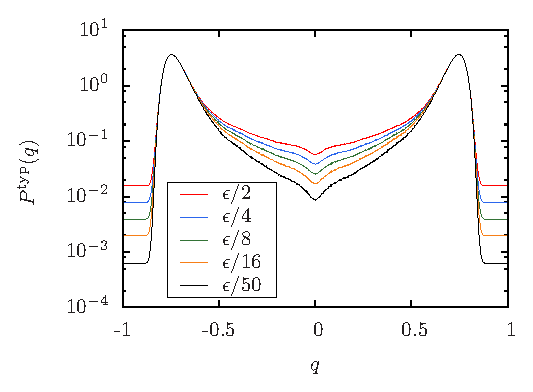
\includegraphics{import/EP}
  \caption
  [
    ``Typical" overlap distribution for the Sherrington-Kirkpatrick spin glass
    for various zero-replacement values $\epsilon/k$.
  ]
  {
    Log-linear plot of $P^{\mathrm{typ}}(q)$ for the SK model with $N=2048$,
    showing the strong dependence on the zero-replacement value $\epsilon/k$.
  }
  \label{fig:pofq-typical-sk}
\end{figure}


\section{Summary and conclusions}

We have studied the overlap distribution for several Ising spin-glass models
using recently-proposed observables. We consider 1D long-range models, 3D and
4D short-range (Edwards-Anderson) models, and the infinite-range
(Sherrington-Kirkpatrick) model. The three observables are all obtained from
the single-sample overlap distribution $P_{\JJ}(q)$. They are the fraction of
peaked samples $\Delta(q_0,\kappa)$, the median of the cumulative distribution
$I^{\mathrm{med}}(q)$, and the typical value of the distribution
$P^{\mathrm{typ}}(q)$. These observables were proposed to help distinguish
between the replica symmetry breaking picture and two-state pictures such as
the droplet model. While none of these unambiguously differentiates between
these competing pictures, it appears that $\Delta$ does the best job. In
particular, there is a qualitative distinction between the behavior for the 3D
EA model and the long-range 1D model with $\sigma=0.896$ that is expected to
mimic it, on the one hand, and the mean-field SK model and the 1D model with
$\sigma=0.6$ that is expected to be in the mean-field regime, on the other
hand. For a reasonable range of $q_0$ and $\kappa$, the two 3D-like models do
not show an increase in $\Delta$ for the largest sizes while the mean-field
models are sharply increasing for the largest sizes. The increase in $\Delta$
for the mean-field model is exactly what we expect from the RSB picture. The
results for the 3D-like models are ambiguous because eventually $\Delta$ must
go either to zero or one. It is possible that for much larger sizes $\Delta$
will begin to increase, indicating RSB behavior, but simulating such large
systems at very low temperatures is infeasible at present.

The other proposed measures do not appear to be useful in numerical simulations
for distinguishing scenarios. The typical value of the overlap distribution,
$P^{\mathrm{typ}}(q)$ cannot be measured in feasible Monte Carlo simulations,
while the median value of the cumulative overlap $I^{\mathrm{med}}(q)$ is very
small at small $q$ even for the SK model and has a very strong size dependence.
For the droplet model $I^{\mathrm{med}}(q)$ is presumably zero at small $q$ for
$N \to \infty$. However, the strong size dependence of the results in this
region of small $q$ makes it impossible to tell numerically if the data are
going to zero or just to a very small value, even for the SK model. Curiously,
there is \emph{less} size dependence for the 3D model and the equivalent 1D LR
model with $\sigma=0.896$ than for the SK model.

In contrast to the findings of \textcite{billoire2014cumulative} that the data
for $I^{\mathrm{med}}(q)$ for the SK model ``converge nicely to some limiting
curve when $N$ increases" and that ``trading the average for the median does
make the analysis more clear-cut," we find a strong size-dependence for
$I^{\mathrm{med}}(q)$ for te SK model in the important small-$q$ region
(clearly visible in a logarithmic scale) and largely because of this we do not
find that the median is particularly helpful in distinguishing between the
droplet and RSB pictures.

\chapter{Connection between dynamics and statics in spin glasses}
\label{chap:connection}

\section{Introduction}
\label{sec:connection-intro}

Theoretical calculations in statistical physics often involve \emph{equilibrium
  averages} over a thermodynamic ensemble, for example the canonical ensemble,
where it is assumed that the system is in equilibrium with a heat bath at fixed
temperature. In contrast, experiments and simulations usually measure
steady-state \emph{time averages}. While such \emph{static} and \emph{dynamic}
averages are usually equivalent, this equivalence can break down.

One case where this may occur is in the ordered phase of a system that exhibits
a phase transition with spontaneous symmetry breaking. For example, consider an
Ising ferromagnet in zero field. As the system is cooled below the transition
temperature, the symmetry of the paramagnetic phase is broken and subsequent
observation will find the system in one of two ordered states, ``up" or
``down," corresponding to the sign of the net magnetization.%
\footnote{%
  Here, by ``state" we mean a \emph{thermodynamic} state, corresponding to a
  probability distribution over the microscopic configurations.
}
These ``up" and ``down" states have the property that spatial correlations of
fluctuations vanish at long distances, \textit{i.e.}
\begin{equation}
  \lim_{r_{ij} \to \infty} \left( \av{S_i S_j} - \av{S_i}\av{S_j} \right) = 0.
  \label{eq:clustering-prop}
\end{equation}
\Cref{eq:clustering-prop} is called a ``clustering property" and states that
satisfy it are called ``pure" states \autocite{newman2003ordering}. The set of
pure states is ``complete" in the sense that \emph{any} thermodynamic state can
be expressed as a linear combination of pure states. More precisely,
correlation functions evaluated in an arbitrary thermodynamic state $\rho$ may
be decomposed as a convex combination%
\footnote{%
  That is, a linear combination where all coefficients are nonnegative and the
  sum of the coefficients is one.
}
of correlation functions, each evaluated in a pure state $\rho_{\alpha}$,
% TODO: reword
\begin{equation}
  \av{S_{i_1} \dots S_{i_n}}_{\rho}
  = \sum_{\alpha} W_{\alpha} \av{S_{i_1} \dots S_{i_n}}_{\rho_{\alpha}},
\end{equation}
where we say that $W_{\alpha}$ is the ``weight" of $\rho_{\alpha}$ in $\rho$.
If a state $\rho$ does not satisfy \cref{eq:clustering-prop}, more than one of
the $W_{\alpha}$ will be nonzero and we say that $\rho$ is a ``mixed" state.

Returning now to the ferromagnet, in an experiment we will find either the
``up" or ``down" state. However, the Boltzmann distribution does not exhibit
the broken symmetry of the ordered phase and includes equal contributions of
both states, giving a net magnetization of zero. Thus \cref{eq:clustering-prop}
is not satisfied and the canonical ensemble corresponds to a \emph{mixed}
state.

However, in spin glasses, which have disorder and ``frustration," the situation
is more complicated. Below the spin glass transition temperature $T_c$, a
macroscopic spin glass is not in thermal equilibrium because relaxation times
are far longer than any experimental time scale. Rather, in a typical
experiment the system is ``quenched" from a high temperature to a temperature
below $T_c$ and the subsequent dynamical evolution of the system is observed.
The state (or states) of thermal equilibrium are very complicated and are not
related to any symmetry.
% contrast with ferromagnet
As for the ferromagnet we would like to find a \emph{static} calculation which
will predict the experimental behavior, at least to some extent. Below we show
\emph{quantitatively} that the theoretical construct called the ``metastate"
\autocite{newman1997metastate,aizenman1990rounding},
combined with the technique of ``replica symmetry breaking" (RSB, see
\cref{sec:intro-rsb}), provides such a description for spin glasses, at least in
dimensions above the upper critical dimension $d_u$, where the critical
behavior is described by mean-field theory.

Pure states, those states that satisfy \cref{eq:clustering-prop}, are
convenient to study for several reasons. As in the case of the ferromagnet with
its ``up" and ``down" states, finding the pure states provides insight into the
nature of the broken symmetry. Furthermore, \emph{pure states are observed in
  experiment}, while mixed states (for example, the canonical ensemble for the
ferromagnet, which has zero magnetization even below $T_c$) are not. Thus we
would like to also describe spin glasses in terms of pure states. This can be
done (in principle) by taking a very large system, applying boundary conditions
on it, and studying the correlations in a relatively small window far from the
boundary \autocite{newman2003ordering,read2014short}. This procedure is
repeated for many different boundary conditions.
% TODO: explain

The question of whether there are many pure states or just one (a time-reversed
pair in the absence of a magnetic field) in spin glasses has been very
controversial.%
% TODO: ref discussion in intro
\footnote{%
  See, for example,
  \textcite{%
    parisi1980order,%
    parisi1983order,%
    fisher1987absence,%
    fisher1988equilibrium,%
    moore2011disappearance%
  }
}
If there are many, one needs to do some sort of statistical average over them,
which is called a ``metastate," for which different but equivalent formulations
have been given by \textcite{newman1997metastate} and by
\textcite{aizenman1990rounding}. In the latter (AW) metastate, one considers
the scale $M$, intermediate between the window size $W$ and the system size
$L$. The metastate-averaged state (MAS) is obtained by computing correlation
functions in a window in which an average is performed not only over the spins
but also over the bonds in the ``exterior" region between $M$ and $L$.
The setup is sketched in \cref{fig:metastates}.%
\footnote{%
  For more details see
  \textcite{%
    aizenman1990rounding,%
    read2014short,%
    manssen2015aging%
  }
}
Parisi's exact solution of the infinite-range Sherrington-Kirkpatrick (SK)
model using RSB predicts many pure states (see \cref{sec:intro-rsb}) in a sense
that was later clarified by \textcite{newman1997metastate}.

\begin{figure}
  \centering
  \begin{subfigure}{0.49\textwidth}
    \centering
    \includestandalone{figures/ns-metastate}
    \subcaption{NS metastate ($W \ll L$)}
    \label{fig:ns-metastate}
  \end{subfigure}
  \begin{subfigure}{0.49\textwidth}
    \centering
    \includestandalone{figures/aw-metastate}
    \subcaption{AW metastate ($W \ll M \ll L$)}
    \label{fig:aw-metastate}
  \end{subfigure}
  \caption[
    The spin-glass metastate as defined by \textcite{newman1997metastate} and
    by \textcite{aizenman1990rounding}.
  ]
  {
    Sketch of the setups for two different (but presumably equivalent)
    formulations of the metastate given by \subref{fig:ns-metastate}
    \textcite{newman1997metastate} and by \subref{fig:aw-metastate}
    \textcite{aizenman1990rounding}.
  } \label{fig:metastates}
\end{figure}

The critical behavior of a realistic spin glass is expected to be the same as
that of the SK model in dimension $d$ greater than the upper critical
dimension, $d_u=6$. However, this does not necessarily mean that the RSB
description of the spin glass phase \emph{below} $T_c$ also applies for $d>6$.%
\footnote{%
  See
  \textcite{%
    newman1997metastate,%
    fisher1987absence,%
    fisher1988equilibrium,%
    moore2011disappearance%
  }
}
Nonetheless, \textcite{read2014short} has computed the spatial fluctuations in a
finite-dimensional model below $T_c$, assuming mean-field (Gaussian) fluctuations,
% TODO: clarify
and the metastate description from Parisi's RSB solution of the SK model. Spin
correlations are found to fall off with a power of distance, due to averaging
over many pure states (which are unrelated by symmetry) in the metastate, \emph{i.e.}
% TODO: expand/clarify
\begin{equation}
  \av{S_i S_j}_{\mathrm{MAS}}^2 \propto r_{ij}^{-\alpha_s}
  \quad\text{with}\quad
  \alpha_s = d - 4,
  \label{eq:corr-decay-static}
\end{equation}
where ``s" stands for ``static," ``MAS" stands for metastate-averaged state,
and sites $i$ and $j$ are in the window far from the boundary. For a detailed
discussion of how to do the metastate average see \textcite{read2014short}.
% TODO: should give some more detail here...

We emphasize that the calculation leading to \cref{eq:corr-decay-static}
is a \emph{static} one.
% TODO: meaning?
Is it possible to relate \cref{eq:corr-decay-static} to experiments (or
numerical simulations), which concern (non-equilibrium) dynamics?
Many simulations%
\footnote{%
  \textcite{%
    manssen2015aging,%
    rieger1993nonequilibrium,%
    marinari1996numerical%
  }
}
have been carried out in which a spin glass is quenched to below $T_c$ and the
resulting dynamics analyzed. It is found that fluctuations can equilibrate (or
at least reach a steady state) on length scales smaller than a dynamic
correlation length $\xi(t)$ which is found, empirically, to grow with a power
of $t$ like
\begin{equation}
  \xi(t) \propto t^{1/z(T)},
  \label{eq:xi-scaling}
\end{equation}
where the non-equilibrium dynamical exponent $z(T)$ varies, roughly, like $1/T$
and becomes close to the critical dynamical exponent $z_c$ for $T=T_c$,
\textit{i.e.}
\begin{equation}
  1/z(T) \simeq (T/T_c) z_c.
\end{equation}
%Recently, though, \textcite{} has argued that $z(T)$ does not precisely equal
%$z_c$ in the limit $T \to T_c$.
% TODO: find ref

At distances less than $\xi(t)$ correlations are observed to fall off with a
power of distance, leading to the following scaling hypothesis,
\begin{equation}
  C_4(r_{ij},t)
  \equiv \dav{\av{S_i(t) S_j(t)}^2}
  =  r_{ij}^{-\alpha_d} f \del{\frac{r}{\xi(t)}},
  \label{eq:c4-scaling}
\end{equation}
where ``d" stands for ``dynamic." Here the square of the thermal average,
$\av{\cdots}^2$, is performed by simulation two copies of the system with the
same interactions, initialized with different random spin configurations.
Use of two copies provides an unbiased estimate of this thermal average.
% TODO: explain / ref earlier discussion
The second average, $\dav{\cdots}$, is over the bonds. We will also average over
all pairs of sites a given distance $r$ apart.

For $r_{ij} \ll \xi(t)$, $f(x)$ approaches a constant as $x \to 0$, so
% TODO: why?
\begin{equation}
  C_4(r_{ij},t) \propto r_{ij}^{-\alpha_d}
  \quad\text{($r_{ij} \ll \xi(t)$)}.
  \label{eq:corr-decay-dynamic}
\end{equation}
In the opposite limit, $r_{ij} \gg \xi(t)$, \emph{i.e.} large $x$, $f(x)$
decreases exponentially for short-range systems.
% TODO: define "short-range" system

Clearly, the nonequilibrium dynamics is generating a sampling the pure states.
To our knowledge, \textcite{white2006scenario} were the first to point out the
similarity of this sampling to the metastate average for statics. They use the
term ``maturation metastate" to describe the ensemble of states generated
dynamically on scales less than $\xi(t)$ following a quench, and ``equilibrium
metastate" for the static metastate discussed earlier. Here we will use the
terms ``dynamic" and ``static" to describe these two metastates. Subsequently
\textcite{manssen2015nonequilibrium} emphasized the similarity between the two
metastates and suggested that they might actually be equivalent, in which case
$\alpha_s$ in \cref{eq:corr-decay-static} would equal $\alpha_d$ in
\cref{eq:corr-decay-dynamic}.

The rationale behind this hypothesis is that thermal fluctuations of the spins
outside the window at a distance $\xi(t)$ and greater, which are not
equilibrated with respect to spins in the window, effectively generate a random
noise to the spins in the window which is similar to the random perturbation
coming from changing the bonds in the outer region according to the AW
metastate.

For the three-dimensional spin glass, \textcite{banos2010nature,banos2010static}
have shown that a static calculation in the zero spin overlap sector
% TODO: explain
gives a power-law decay for the spin correlations, as in
\cref{eq:corr-decay-static}, with a value of $\alpha_s$ consistent with that
obtained from dynamcs following a quench by \textcite{belletti2009depth}. These
are both numerical results. Here we consider the mean-field regime, $d>6$,
because there is an exact \emph{analytic} result in RSB theory, $\alpha_s=d-4$,
with which we can compare our numerical results.


\section{Model}

Unfortunately, it is difficult to carry out Monte Carlo simulations of spin
glasses in in six dimensions (see the discussion in
\cref{sec:nonextensive-motivation}). Instead, we study the \emph{diluted}
one-dimensional models with long-range interactions described in
\cref{sec:nonextensive-models}, which we briefly review here. The
one-dimensional diluted model is described by the Hamiltonian
\begin{equation}
  \ham = -\sum_{i,j} J_{ij} S_i S_j,
\end{equation}
where the sites $i\in\cbr{1,2,\dots,N}$ lie on a one-dimensional ring with
periodic boundary conditions, as shown in \cref{fig:1dlr-chord}. The variables
$S_i = \pm 1$ are Ising spins, and the interactions $J_{ij}$ are independent
random variables with a distribution satisfying
\begin{equation}
  \dav{J_{ij}}=0,\qquad
  \dav{J_{ij}^2} \propto R_{ij}^{-2\sigma},
  \label{eq:J-mean-variance-lr-2}
\end{equation}
where $R_{ij}$ is taken to be the chord distance between sites $i$ and $j$, see
\cref{fig:1dlr-chord}. We vary the parameter $\sigma$ to control the range of
the interactions.

The \emph{diluted} model corresponds to a particular choice of the distribution
$P(J_{ij})$ that satisfies \cref{eq:J-mean-variance-lr-2} while allowing for
efficient simulation, namely
\begin{equation}
  P(J_{ij})
  = \del{1 - p_{ij}} \delta \del{J_{ij}}
  + p_{ij} \frac{1}{\sqrt{2\pi}} e^{-J_{ij}^2/2}.
  \label{eq:dilute-dist-2}
\end{equation}
See \cref{sec:nonextensive-models} for a detailed discussion of the diluted
model and an algorithm to sample from \cref{eq:dilute-dist-2}.

As discussed in \cref{sec:nonextensive-motivation}, varying the parameter
$\sigma$ is argued to be analogous to changing the dimension $d$ of a
short-range model. In the mean-field regime, $d>d_u=6$ for the short-range
model, a precise connection can be given between $\sigma$ and an equivalent
$d$, namely
\begin{equation}
  d = \frac{2}{2\sigma - 1}
  \label{eq:d-sigma}
\end{equation}
(see \cref{sec:nonextensive-motivation}), and thus, for the long-range model,
the mean-field regime is $1/2 < \sigma < 2/3$.

The connection between critical exponents of the short-range and corresponding
long-range models has been discussed systematically by
\textcite{banos2012correspondence}, who note that an exponent of the
short-range model in $d$ dimensions is $d$ times the corresponding exponent of
the equivalent one-dimensional long-range model.
% TODO: explain
Thus, to get the exponent $\alpha_s=d-4$ in the static metastate for the
long-range model we divide by $d$ and, since we will work in the mean-field
regime, use \cref{eq:d-sigma} to relate $d$ to $\sigma$. This gives
\begin{equation}
  \alpha_s = 3-4\sigma
  \quad\text{(long-range model).}
  \label{eq:alpha-rsb-lr}
\end{equation}

In this work we focus on a single value of $\sigma$ in the mean-field regime,
$\sigma=5/8$, which corresponds to $d=8$ according to \cref{eq:d-sigma}. Using
standard finite-size scaling analysis (see \cref{sec:numerical-fss}) we find
that $T_c=1.85(2)$ for this model with $z_b=6$.
% TODO: define z_b
Here we need to work \emph{well} below $T_c$ so that our data is characteristic
of the ordered phase and does not also incorporate critical fluctuations.
Thus we take $T = 0.4 T_c = 0.74$ for the simulations.


\section{Method}

We quench the system from infinite temperature to $T=0.74$ at time $t=0$ and
follow the evolution of the system using Monte Carlo simulation with only local
(\textit{e.g.} \emph{not} replica exchange) updates. We measure spin
correlations, averaging them for times between $2^{k-1}$ and $2^k$, for integer
$k$ up to the maximum value. For the largest sizes this was $k=14$. We find
that finite-size effects are very large and we need to study enormously large
sizes. We therefore take a range of sizes which also increases geometrically,
$N=2^{\ell}$ up to $\ell=26$. We also average over about 1000 samples (the
precise number depending on size).
% TODO: table of simulation params


\section{Results}

\Cref{fig:c4-vs-r-sizes} shows our data for the correlation function $C_4(r,t)$,
defined in \cref{eq:c4-scaling}, as a function of $r\equiv\abs{i-j}$ at
$t=2^{14}$ for different sizes. Despite the strong finite-size effects, the data
seems to have saturated for the largest sizes, at least for the range of distance
presented.
\begin{figure}
  \centering
  \includestandalone{figures/c4-vs-r-sizes}
  \caption[
    Data for the correlation function averaged between $t=2^{13}$ and $2^{14}$
    for different sizes of the 1-d long-range diluted spin glass with
    $\sigma=5/8$ at $T=0.4T_c$.
  ]
  {
    Data for the correlation function $C_4(r,t)$, defined in \cref{eq:c4-scaling},
    as a function of $r$ for the range of sizes studied. The data is averaged
    between $t=2^{13}$ and $2^{14}$.
  } \label{fig:c4-vs-r-sizes}
\end{figure}

Having established that the largest size, $N=2^{26}$, is large enough to
eliminate finite-size effects for the range of $r$ and $t$ considered, we now
discuss the data for this size in detail. \Cref{fig:c4-vs-r-times} shows data
for $C_4(r,t)$ at different times as a function of $r$. It is expected to have
the scaling form shown in \cref{eq:c4-scaling}. For short-range models, the
scaling function $f(x)$ decays exponentially at large $x$ because the
correlation function falls off very rapidly once $r$ is greater than the
dynamical correlation length. However, in the present model we have
interactions of arbitrarily long range which give a ``direct" contribution to
the correlation function at large distances. Since $C_4(r,t)$ involves the
square of the spin-spin correlation function, and is averaged over the
interactions, the direct contribution should be proportional to
$\dav{J_{ij}^2}$, which, according to \cref{eq:J-mean-variance-lr-2}, is
proportional to $r^{-2\sigma}$ ($=r^{-5/4}$ for $\sigma=5/8$). The data in
\cref{fig:c4-vs-r-times} follow this behavior for short times and large
distances, see the dotted line.

By contrast, at small $r$ and large $t$, where $r \ll \xi(t)$, the data for
different times collapse and are consistent with a decay proportional to
$r^{-(3-4\sigma)}$ ($=r^{-1/2}$ for $\sigma=5/8$), see the dashed line in
\cref{fig:c4-vs-r-times}. To better estimate the slope at large $t$ and small
$r$ we plot in the inset to \cref{fig:c4-scaling} the ``effective" exponent
$\alpha_{\mathrm{eff}}$, the slope of the data in \cref{fig:c4-vs-r-times}, as
a function of $r$ for different times. The curves are quadratic fits for
intermediate $r$ ($7 \leq r \leq 255$). The intercepts of the fits approach
$-1/2$ for $r \to 0$ at large $t$. Thus, according to
\cref{eq:corr-decay-dynamic}, we have $\alpha_d=3-4\sigma$ (or at least very
close to it). However, this is precisely equal to $\alpha_s$, the corresponding
exponent from the \emph{static} metastate according to RSB theory as shown in
\cref{eq:alpha-rsb-lr}. Thus we see that, in the mean-field regime, the static
and dynamic metastates appear to agree and the description appears to be that
of RSB. The latter is in agreement with several other studies
\autocite{moore2011disappearance,katzgraber2005probing} and is of course also
implied by those, such as \textcite{banos2010nature,banos2010static}, which
argue that RSB holds even below six dimensions.
\begin{figure}
  \centering
  \includestandalone{figures/c4-vs-r-times}
  \caption[
    Data for the correlation function at different times of the 1-d long-range
    diluted spin glass with $\sigma=5/8$ at $T=0.4T_c$.
  ]
  {
    Data for the correlation function for the largest size $N=2^{26}$ as a
    function of $r$ for different times. A gradual crossover can be seen
    between two power laws. At long times and short distances $C_4(r,t) \propto
    1/r^{\alpha_d}$ with $\alpha_d = 3 - 4\sigma$ (dashed line); at short times
    and long distances $C_4(r,t) \propto 1/r^{-2\sigma}$ (dotted line) which is
    just the average of the square of the interactions $J_{ij}$.
  } \label{fig:c4-vs-r-times}
\end{figure}

The main part of \cref{fig:c4-scaling} shows a scaling plot of our data for the
largest size according to \cref{eq:c4-scaling,eq:xi-scaling}. The data scale
well with $z(T)=1.4$ and, including estimated error bars, we have the result
$z(0.4 T_c)=1.4(2)$ for the dynamical exponent describing the growth of
nonequilibrium correlations following a quench. For short-range models it is
found empirically%
\footnote{%
  \textcite{%
    manssen2015aging,%
    rieger1993nonequilibrium,%
    % TODO: missing ref
    marinari1996numerical,%
    yoshino2002extended%
  }
}
that $1/z(T) \propto T$. If we assume the same here then $z(T_c)=0.56(8)$.
Furthermore, still for short-range models it is also found that $z(T_c)$,
obtained from nonequilibrium data, is equal to (or at least close to)
the equilibrium dynamical exponent $z_c$. We therefore take $z_c=0.56(8)$
for our long-range model. To translate this into the exponent for the
equivalent short-range model, we multiply by $d$ ($=8$), as discussed above,
so our estimate for the critical dynamical exponent of the $d=8$ short-range
spin glass is $z_c=4.5(6)$ ($d=8$). This model is in the mean-field regime
($d>6$) for which the dynamical exponent is found to be $z_c=4$
\autocite{zippelius1984critical}. Our result is consistent with this.

\begin{figure}
  \centering
  \includestandalone{figures/c4-scaling}
  \caption[
    Scaling plot of data for the dynamical correlation function $C_4(r,t)$ at
    different times for the 1-d long-range diluted spin glass with
    $\sigma=0.74$ at $T=0.4T_c$.
  ]
  {
    Scaling plot of the data for the largest size $N=2^{26}$ at $T=0.74$
    according to \cref{eq:c4-scaling}. The inset shows the effective exponent
    $\alpha_{\mathrm{eff}}$, the slope of the curves in
    \cref{fig:c4-vs-r-times}, as a function of $r$. The curves in the inset are
    quadratic fits to the data for intermediate $r$, $7 \leq r \leq 255$. The
    intercepts of the fits approach $-0.5$ at long times.
  }
  \label{fig:c4-scaling}
\end{figure}


\section{Conclusion}

We have shown quantitatively that the nonequilibrium dynamics following a
quench of a model which is a proxy for a short-range spin glass in dimension
$d>6$ is given, in the steady-state regime where the distance is less than the
nonequilibrium correlation length, by the \emph{analytic} result for the
\emph{static} metastate calculated according to RSB theory. This suggest that
(i) RSB theory applies to spin glasses above the upper critical dimension,
$d_u=6$, and (ii) the dynamic and static metastates are equivalent (at least in
this region).

\chapter{Finite-size scaling above the upper critical dimension}
\label{chap:fss}

\section{Introduction}
\label{sec:fss-intro}

The theory of finite-size scaling (FSS) bridges the gap between the critical
behavior of \emph{finite} systems and that of infinite (or effectively
infinite) systems which are commonly studied in analytical theory and
experiment. As such, FSS is ubiquitous in the literature of computational
physics, where it is used extensively to extrapolate \emph{bulk} (\emph{i.e.}
$L\to\infty$) behavior, which can be compared with analytical or experimental
results, from the results of numerical simulation of finite systems
\autocite{binder2001monte}.
% TODO: awkward ^

As discussed in \cref{sec:numerical-fss}, the central assumption of
\emph{standard} FSS is that finite-size corrections only involve the ratio of
the system size $L$ to the bulk (\emph{i.e.} infinite system size) correlation
length $\xi$.
% TODO: ref for this?
While this assumption turns out to be correct in dimensions $d$ less than the
upper critical dimension $d_u$, the situation is more complicated \emph{above}
the upper critical dimension, $d>d_u$. This is a bit surprising since for
$d>d_u$ the critical exponents are independent of $d$ and are predicted exactly
by mean-field theory. Thus, we might naively expect from
\cref{eq:standard-fss-susc} that, for $d>d_u$, the susceptibility scales with
$L$ like
\begin{equation}
  \chi(L,T) \sim L^2 \scalefunc{\chi}\sbr{L^2 \del{T-T_c}},
  \label{eq:fss-above-naive}
\end{equation}
where $\scalefunc{\chi}$ is a scaling function and we have inserted the
mean-field exponents $\gamma=1$ and $\nu=1/2$. Unfortunately, it is not that
simple, and instead it turns out that the basic assumption of FSS, that $L$
dependence enters only through the ratio $L/\xi$, is invalid for $d>d_u$. The
trouble is related to the observation that, for $d>d_u$, ``hyperscaling"
relations such as $d \nu = \gamma - 2\beta$ are necessarily violated, since the
critical exponents ``stick" at their mean-field values for all values of
$d>d_u$. It turns out that a ``dangerous irrelevant variable" is responsible
for both effects. To understand this we need a more sophisticated approach
based on the renormalization group (RG).

According to renormalization-group derivations of FSS
\autocite{privman1983finite}, the singular part of the free energy $f_L$ and
the correlation length $\xi_L$ have the form
\begin{align}
  f_L &= L^{-d} \scalefunc{f}\del{t L^{y_t}, h L^{y_h}, u L^{y_u}}, \\
  \xi_L &= L \scalefunc{\xi}\del{t L^{y_t}, h L^{y_h}, u L^{y_u}},
\end{align}
where $t\equiv(T-T_c)/T_c$ is the reduced temperature, $h$ is the magnetic
field, and $u$ is the quartic coupling of the Landau theory; $y_t$, $y_h$, and
$y_u$ are the corresponding renormalization-group exponents.
For $d < d_u$, $u$ is a relevant variable ($y_u > 0$, see \cref{sec:intro-landau})
and for $h=0$ we obtain the scaling forms
\begin{subequations}
\begin{align}
  \chi(L,t) &= L^{\gamma y_t} \scalefunc{\chi}\del{t L^{y_t}}
  \label{eq:fss-standard-susc} \\
  g(L,t) &= \scalefunc{\chi}\del{t L^{y_t}},
\end{align}
\label{eq:fss-standard}
\end{subequations}
where $y_t=1/\nu$, for the susceptibility and Binder ratio [defined in
\cref{eq:binder}] respectively.

For $d > d_u$, $u$ is irrelevant ($y_u<0$), but the corresponding derivation is
complicated by the fact that the scaling function $\scalefunc{f}(x,y,z)$ is
singular in the limit $z \to 0$, \textit{i.e.}, $u$ is a \emph{dangerous
  irrelevant variable}. Therefore we can't simply substitute $z=0$ in the
scaling function, and must instead evaluate the limit $z \to 0$, assuming a
particular form of the singularity.


\subsection{Periodic boundary conditions}

For $k=0$ fluctuations%
\footnote{%
  \emph{i.e.}, fluctuations in the $k=0$ mode of the order parameter, for
  example in the (uniform) magnetization, $\sum_i S_i$.
}
in systems with periodic boundary conditions, \textcite{binder1985finite} show
that, for $d>d_u$, the thermal exponent $y_t$ is replaced by $y_t^*$,
\begin{subequations}
\begin{align}
  \chi(L,t) &= L^{y_t^*} \scalefunc{\chi}\del{L^{y_t^*} t},
  \label{eq:fss-above-susc} \\
  g(L,t) &= \scalefunc{\chi}\del{L^{y_t^*} t},
  \label{eq:fss-above-binder}
\end{align}
\label{eq:fss-above}
\end{subequations}
where
\begin{equation}
  y_t^*=d/2.
  \label{eq:fss-above-yt}
\end{equation}
% TODO: underlying assumption gives correct bulk behavior in all limiting cases
This is a surprising result because it predicts that finite-size corrections
appear not when $\xi \sim L$, as is assumed in standard FSS, but rather only
when $\xi \sim L^{d/4}$, a length scale larger than the size of the system.%
\footnote{
  To see this, note that for $d > d_u$, $t \sim \xi^{-1/\nu} = \xi^{-2}$, so
  the argument of the scaling function $L^{y_t^*} t = L^{d/2} \xi^{-2}$ is of
  order unity when $\xi \sim L^{d/4}$.
}
Consequently, the finite-size transition is ``rounded out" over a temperature
range which scales like $L^{-d/2}$, smaller than $L^{-2}$ predicted by standard
FSS.

An extensive set of works%
\footnote{%
  For example,
  \textcite{
    luijten1996finite,
    parisi1996scaling,
    blote1997universality,
    luijten1999finite,
    binder2001monte,
  }
}
have shown the validity of \cref{eq:fss-above}, though it required large system
sizes, good statistics, and appreciation that \emph{corrections} to FSS are
large and slowly decaying for the range of sizes that can feasibly be
simulated.
%The (universal) value $\scalefunc{g}(0)$, computed by
%\textcite{brezin1985finite} (who showed it to be simply that obtained by
%including \emph{only} the $k=0$ mode with $T_c$ adjusted to the correct value)
%has been confirmed.
% TODO: wording/correctness ^
% TODO: understand this ^


\subsection{Free boundary conditions}

As stated above, \cref{eq:fss-above} makes the rather surprising prediction
that, for $d>d_u$ and periodic boundary conditions, finite-size effects set in
not when $\xi \sim L$, but even closer to criticality, when $\xi \sim L^{d/4}$.
It is therefore interesting to ask what is the corresponding behavior for free
boundary conditions, where we expect that \emph{something} must happen when the
correlation length $\xi \sim L$ \autocite{jones2005finite}. In fact,
\textcite{rudnick1985effect} have argued analytically that a temperature
\emph{shift} of order $L^{-2}$ has to be included with free boundary
conditions, in addition to the rounding of order $L^{-d/2}$.

To explain this, note that the exponents $y_t$ in \cref{eq:fss-standard} and
$y_t^*$ in \cref{eq:fss-above} are ``rounding" exponents since they control the
temperature range over which a singularity is rounded out. To define the
``shift" exponent, we first define, for each size $L$, a ``finite-size
pseudocritical temperature" $T_L$ by, for example, the location of the peak in
some susceptibility, or the temperature at which the Binder ratio [defined in
\cref{eq:binder}] has a particular value. The difference $T_c-T_L$ goes to zero
for $L\to\infty$ like
\begin{equation}
  T_c - T_L = \frac{A}{L^{\lambda}},
  \label{eq:TL-scaling}
\end{equation}
defining the shift exponent $\lambda$. The precise value of $T_L$ depends on
which criterion is used to define it, but the exponent $\lambda$ is expected to
be independent of the definition. Whether or not the amplitude $A$ depends on
the quantity used to define the shift will be discussed in
\cref{sec:fss-results-fbc}.
% TODO: redundant/contradictory? ^

If $\lambda$ is less than the rounding exponent, which will turn out to be the
case for free boundary conditions, then the shift is \emph{larger} than the
rounding, so we need to modify \cref{eq:fss-above} to
\begin{subequations}
\begin{align}
  \chi(L,t) &= L^{y_t^*} \scalefunc{\chi}\sbr{L^{y_t^*}\del{T-T_L}},
  \label{eq:fss-above-shift-susc} \\
  g(L,t) &= \scalefunc{\chi}\sbr{L^{y_t^*}\del{T-T_L}},
  \label{eq:fss-above-shift-binder}
\end{align}
\label{eq:fss-above-shift}
\end{subequations}
in which the argument of the scaling function involves the difference between
$T$ and the pseudocritical temperature $T_L$. We verify
\cref{eq:fss-above-shift} in
\cref{fig:qshift,fig:qwidth,fig:qchiTL,fig:chi-f-scaling} below.

The criterion that the shift is given by the (standard FSS) condition $\xi \sim
L$ yields $\lambda=2$, as proposed by \textcite{rudnick1985effect} and
confirmed in simulations by \textcite{berche2012hyperscaling,kenna2013new}. As
with \cref{eq:fss-standard-susc} we must have $\scalefunc{\chi}(x) \propto
x^{-1}$ for $x \to \infty$ in order to recover the correct bulk behavior above
$T_c$. Setting $T=T_c$, we have
\begin{equation}
  \chi(L,T_c) = L^{d/2}\scalefunc{\chi}(A L^{d/2-2}),
\end{equation}
and therefore, asymptotically for large $L$,
\begin{equation}
  \chi(L,T_c) \propto L^2
  \quad\text{(free, $k=0$)},
  \label{eq:rounding-k0-Tc}
\end{equation}
a result that has been shown rigorously.
% TODO: reference
Hence, in contrast to \textcite{berche2012hyperscaling}, we propose that the
region at the bulk $T_c$ is part of the scaling function.
% TODO: explain "part of"
Similarly, for the Binder ratio, $\scalefunc{g}(x) \propto x^{-2}$
% TODO: why?
for $x\to\infty$, which gives
\begin{equation}
  g(L,T_c) \propto \frac{1}{L^{d-4}}
  \quad\text{(free, $k=0$)}.
  \label{eq:binder-scaling-Tc}
\end{equation}
With periodic boundary conditions, the intersection of the data for $g$ for
different sizes provides a convenient estimate of $T_c$, but, as
\cref{eq:binder-scaling-Tc} shows, this method cannot be used for free boundary
conditions because $g$ vanishes at $T_c$ for $L\to\infty$. In fact, we will see
from the data in \cref{sec:fss-results-fbc} that there are no intersections at
all. However, we will not be able to verify the precise form in
\cref{eq:binder-scaling-Tc} because the values of $g$ at $T_c$ are very small,
below the noise threshold of our simulations.

So far we have discussed only $k=0$ fluctuations. However, it is also necessary
to discuss fluctuations at $\vec{k}\neq\vec{0}$, since we need these to
determine the spatial decay of the correlation functions.
% TODO: explain
Of particular importance is the decay of the correlations at $T_c$, which fall
off with distance like $1/r^{d-2+\eta}$, where the mean-field value of the
$\eta$ exponent is zero.
% TODO: mention anomalous dimension?
In the mean-field regime ($d>d_u$), the fluctuations of the $k=0$ modes are
Gaussian, so the Binder ratio is always zero.
% TODO: explain
For the wavevector-dependent susceptibility, we will argue that \emph{standard}
FSS, \cref{eq:fss-standard-susc}, holds for both boundary conditions (BCs),
\emph{i.e.}
\begin{equation}
  \chi(\vec{k},L,T) =
  L^2 \scalefunc{\chi}\sbr{L^2 \del{T-T_c}, kL}
  \quad\text{(both BCs, $\vec{k}\neq\vec{0}$)},
  \label{eq:susc-kn-scaling}
\end{equation}
where we have put the explicit $k$ dependence in a natural way as a second
argument of the scaling function. We note that \cref{eq:susc-kn-scaling} holds
for the spherical model%
\footnote{%
  Eq.~(22) of \textcite{shapiro1986fully} and Eq.~(37) of
  \textcite{brezin1982investigation} correspond to
  \cref{eq:susc-kn-scaling} with
  $\scalefunc{\chi}(x,y)=\del{x^2+y^2}^{-1}$, at least above $T_c$.
}
with periodic boundary conditions.%
\footnote{%
  The spherical model, in which the length constraint $S_i^2=1$ on each spin is
  replaced by a \emph{single} global average constraint, is equivalent to an
  $n$-component vector model in the limit of $n\to\infty$ for the case of
  periodic boundary conditions. For free boundary conditions, however, the
  correspondence does not hold. In that case, due to a lack of translational
  invariance, one would need a \emph{different} average constraint on each spin
  to reproduce the results of the vector model with an infinite number of
  components.
}
For free boundary conditions, the Fourier modes are not plane waves (see
\cref{sec:fss-model}), and, by $\vec{k}\neq\vec{0}$, we really mean modes that
are orthogonal to the uniform ($k=0$) magnetization and thus do not develop a
nonzero expectation value below $T_c$.

If we fix $T=T_c$ in \cref{eq:susc-kn-scaling} and consider $k L \gg 1$, then
the size dependence must drop out, so $\scalefunc{\chi}(0,y) \propto y^{-2}$
and therefore
\begin{equation}
  \chi(\vec{k},L,T_c) \propto \frac{1}{k^2}
  \quad\text{($k L \gg 1$)}.
  \label{eq:susc-kn-Tc-scaling}
\end{equation}
How, then, do correlations fall off in real space at criticality? To fully
understand this, we have to consider separately the contribution from the $k=0$
mode, as in Bose-Einstein condensation.
% TODO: explain
If $C(\vec{r})$ is the spin-spin correlation function at displacement $\vec{r}$
and $\widetilde{C}(\vec{k})$ is the Fourier transform (FT), then, as shown in
\cref{eq:susc-kn-scaling},
\begin{equation}
  \widetilde{C}(\vec{k}) \propto \frac{1}{k^2}
  \label{eq:ft-corr-kn}
\end{equation}
for $k \to 0$. However, for $k=0$ we note that $\widetilde{C}(k=0) =
\chi(L,T)/L^d$, see \cref{eq:susc-k0} below, and from \cref{eq:fss-above-susc}
this gives
\begin{equation}
  \widetilde{C}(k=0) \propto \frac{1}{L^{d/2}}.
\end{equation}
The real-space correlation function at distance $L/2$ is then given by the FT
\begin{equation}
  C(\vec{\hat{z}}L/2) =
  \del{\frac{L}{2\pi}}^d
  \int_{\vec{k}\neq\vec{0}}\dif^d k\,
  \widetilde{C}(\vec{k})\exp\del{i\vec{k} \cdot L\vec{\hat{z}}/2}
  + \widetilde{C}(k=0).
  \label{eq:rs-corr}
\end{equation}
% TODO: what is zhat?
Using \cref{eq:ft-corr-kn}, which correctly gives the FT at large $r$, the
first term in \cref{eq:rs-corr} is proportional, on dimensional grounds, to
$1/L^{d-2}$. This is smaller than the second term, which is proportional to
$1/L^{d/2}$. Thus, $C(\vec{\hat{z}}L/2) \propto 1/L^{d/2}$, in agreement with
Fig.~1 of \textcite{kenna2014fisher}. Nonetheless, correlations fall off with
distance like $1/r^{d-2}$. The resolution of this apparent discrepancy is that
the $k=0$ mode has to be treated separately and gives the dominant contribution
to $C(\vec{\hat{z}}L/2)$. We therefore do not see the need for the second
$\eta$-like exponent proposed by \textcite{kenna2014fisher}.
% TODO: reword/expand on this paragraph ^

While \cref{eq:susc-kn-scaling} does not seem to have been stated in the
literature before, to our knowledge, it is actually quite natural. The
dangerous irrelevant variable, which is the quartic coupling in the
Ginzburg-Landau-Wilson effective Hamiltonian, is needed to control the
expectation value of the ($k=0$) order parameter, which leads to nonstandard
FSS for $k=0$ fluctuations. However $\vec{k}\neq\vec{0}$ fluctuations (more
precisely, fluctuations that do not acquire a nonzero expectation value) are
not directly affected by the dangerous irrelevant variable, and consequently
they have standard FSS.

% TODO: plan of paper?

\section{Model}
\label{sec:fss-model}

We consider an Ising model in $d=5$ dimensions in zero field, described by the
Hamiltonian
\begin{equation}
  \ham = -\frac{1}{2} \sum_{ij} J_{ij} S_i S_j,
\end{equation}
where the $J_{ij}=1$ if $i$ and $j$ are nearest neighbors and zero otherwise,
and the spins $S_i$ take values $\pm 1$. Previous simulations have determined
the transition temperature very precisely, finding
\begin{equation}
  T_c = 8.77846(3)
  \label{eq:Tc-d5}
\end{equation}
\autocite{luijten1999finite}. We simulate the model efficiently using the Wolff
cluster algorithm described in \cref{sec:numerical-cluster}, with which we can
study sizes up to $L=64$ (which has about a billion spins).
% TODO: L=64 results included?

We calculate various moments of the uniform magnetization per spin,
\begin{equation}
  m = \frac{1}{L^d} \sum_{i=1}^N S_i,
  \label{eq:mag-k0}
\end{equation}
including the uniform susceptibility%
\footnote{%
  This expression differs from the standard expression for the susceptibility
  $\chi=\beta L^d \del{\av{m^2}-\av{m}^2}$ in two ways. The first is that we
  omit the factor of $\beta$, which is conventional in studies of critical
  phenomena. Secondly, and less trivially, we ignore the subtracted term, which
  is hard to compute reliably in Monte Carlo simulations since one would have
  to apply a field $h$ (to break the symmetry) and take the limit $h \to 0$
  \emph{after} the limit $L\to\infty$. Thus the quantity we call $\chi$ is
  really only the susceptibility for $T>T_c$. It is, nonetheless, a convenient
  quantity to study, and it has the claimed scaling behavior.
}
\begin{equation}
  \chi = L^d \av{m^2}
  \label{eq:susc-k0}
\end{equation}
and the Binder ratio
% TODO: ref intro description of Binder ratio?
\begin{equation}
  g = \frac{1}{2}\del{3 - \frac{\av{m^4}}{\av{m^2}^2}}.
  \label{eq:binder}
\end{equation}
In addition, we compute the wavevector-dependent susceptibilities
\begin{equation}
  \chi(\vec{k}) = L^d \av{\abs{m(\vec{k})}^2},
\end{equation}
in which the wavevector-dependent magnetization, $m(\vec{k})$, is defined
differently for periodic and free boundary conditions as follows.

For periodic boundary conditions, the Fourier modes are plane waves,
so we have
\begin{equation}
  m(\vec{k}) = \frac{1}{N} \sum_i e^{i\vec{k}\cdot\vec{r}} S_i
  \quad\text{(periodic)},
\end{equation}
where
\begin{equation}
  k_{\alpha} = 2\pi n_{\alpha}/L
  \quad\text{(periodic)},
\end{equation}
where $n_{\alpha}\in\cbr{0,1,\dots,L-1}$ and $\alpha$ denotes a Cartesian
coordinate.

For free boundary conditions, the Fourier modes are sine waves,
\begin{equation}
  m(\vec{k}) = \frac{1}{N} \sum_i
  \sbr{\prod_{\alpha=1}^d \sin\del{k_{\alpha},r_{i,\alpha}}} S_i
  \quad\text{(free)},
  \label{eq:modes-free}
\end{equation}
where
\begin{equation}
  k_{\alpha} = \pi n_{\alpha}/(L+1)
  \quad\text{(free)},
  \label{eq:allowed-free}
\end{equation}
where $n_{\alpha}\in\cbr{1,2,\dots,L}$ and the components of the lattice
position $r_{i,\alpha}$ also take values between 1 and $L$. There is zero
contribution to the sum in \cref{eq:modes-free} if we set $r_{i,\alpha}=0$ or
$L+1$, so \cref{eq:modes-free,eq:allowed-free} correctly incorporate free
boundary conditions.

Note that $k=0$ is not an allowed mode with free boundary conditions, so the
uniform magnetization in \cref{eq:mag-k0} does not correspond to a single
Fourier mode in this case. Note also that modes with \emph{all} $n_{\alpha}$
odd have a projection onto the uniform magnetization and so will acquire a
nonzero expectation value below $T_c$ in the thermodynamic limit. Such modes
will therefore be subject to the nonstandard FSS in \cref{eq:fss-above}.
However, if any of the $n_{\alpha}$ are even, there is no projection onto the
uniform magnetization, so they will not acquire an expectation value below
$T_c$ and will therefore be subject to the standard FSS in
\cref{eq:susc-kn-scaling}.


\section{Quotient method}
\label{sec:fss-quotient}

The discussion in \cref{sec:fss-intro} assumed that the sizes are
sufficiently large and $T$ sufficiently close to $T_c$ that corrections to FSS
are negligible. For free boundary conditions, however, a substantial fraction
of the spins lie on the surface, so \emph{corrections} to FSS are quite large
and need to be included in the analysis. In this section, we describe the
method we used to include the \emph{leading} corrections to FSS.

A convenient way to extract the leading scaling behavior from the data, in the
presence of corrections, is the quotient method
\autocite{ballesteros1996finite}, based on the phenomenological scaling of
\textcite{nightingale1976scaling}. As an example, consider the deviation of the
pseudocritical temperature $T_L$ from $T_c$ for which the FSS form is given in
\cref{eq:TL-scaling}. Including the \emph{leading} correction to scaling, which
involves a universal exponent $\omega$, we have
\begin{equation}
  \Delta T(L) \equiv T_c - T_L =
  \frac{A}{L^{\lambda}}\del{1 + \frac{B}{L^{\omega}}}.
  \label{eq:shift}
\end{equation}
We determine the quotient $Q\sbr{\Delta T}$ by taking the logarithm of the
ratio of the result for sizes $L$ and $s L$, where $s$ is a simple rational
fraction such as $2$ or $3/2$,
\begin{equation}
  Q_{s,L}\sbr{\Delta T}
  = \frac{1}{\log s} \log\del{\frac{\Delta T(s L)}{\Delta T(L)}}.
  \label{eq:qshift}
\end{equation}
According to \cref{eq:shift} we have, for large $L$,
\begin{equation}
  Q_{s,L}\sbr{\Delta T} = -\lambda + \frac{C_s}{L^{\omega}}
  \label{eq:qshift-scaling}
\end{equation}
where
\begin{equation}
  C_s = \frac{s^{-\omega} - 1}{\log s} B.
\end{equation}
If the data are of sufficient quality, we can fit all of the unknown
parameters. In \cref{eq:qshift-scaling}, these are the exponents $\lambda$,
$\omega$, and the amplitude $C_s$. In most cases, however, we will need to
assume the predicted value for the correction exponent $\omega$ (see below) to
obtain an unambiguous fit for the remaining parameters.

According to the renormalization group, for $d > d_u = 4$, the leading
irrelevant variable has scaling dimension
\begin{equation}
  \omega = d - 4.
\end{equation}
% TODO: understand this
However, for $k=0$ fluctuations and periodic boundary conditions, it was shown
by \textcite{brezin1985finite} that there is an additional, and larger,
correction for finite-size effects with an exponent given by
\begin{equation}
  \omega^{\prime} = \frac{d-4}{2}.
  \label{eq:correction-k0}
\end{equation}
An intuitive way to see this is to note that the ``naive" variation of $\chi$
with $L$ at the critical point, $\chi \propto L^2$ [see
\cref{eq:fss-above-naive}], although not the dominant contribution [which is
$L^{d/2}$ as shown in \cref{eq:fss-above-susc}], is nonetheless still present
as a correction. This correction is down by a factor of $L^{2-d/2}$
($=L^{-\omega^{\prime}}$) relative to the dominant term. We will therefore use
$\omega^{\prime}$ rather than $\omega$ in considering corrections to scaling
for susceptibilities that scale with $L$ to the power $d/2$ rather than 2.
% TODO: understand this

For some of our data, we will also need subleading corrections to FSS for which
there are several contributions. One of these is the square of the leading
contribution. To avoid having too many fit parameters, this is the form we will
assume, \emph{i.e.}, when we include subleading corrections to scaling we will
do a parabolic fit in $1/L^{\omega}$ (or $1/L^{\omega^{\prime}}$ as the case
may be).

A subtlety arises in doing fits to data for quotients, for example to determine
the parameters $\lambda$, $\omega$, and $C_s$ in \cref{eq:qshift-scaling}. The
reason is that the same set of simulation data may be used to determine more
than one data point in the fit. For example, with $s=2$ the data for $L=16$ is
used in the computation of quotients for pairs (8, 16) and (16, 32).
Furthermore, we will fit the exponents $\lambda$ and $\omega$ simultaneously to
quotients for two different values of $s$ ($s=2$ and 3/2),%
\footnote{%
  This is justified since the exponents are universal. The amplitude $C_s$ is,
  however, nonuniversal, so we include a separate amplitude for each value of
  $s$.
}
so for example we also use the data for $L=16$ to compute the quotient for the
pair (16, 24). This has the advantage of increasing the number of data points
in the fit by more than the number of parameters. However, in this case the
data being fitted are \emph{not statistically independent}, and therefore the
best estimate of the fitting parameters should account for the correlations.
\autocite{ballesteros1996finite,ballesteros1998critical,weigel2009cross}. In
other words, if a data point is $(x_i,y_i)$ and the fitting function is $u(x)$,
which depends on certain fitting parameters, those parameters should be
determined by minimizing
\begin{equation}
  \chi^2 = \sum_{i,j}
  \sbr{y_i - u(x_i)}
  \del{\vec{\Sigma}^{-1}}_{ij}
  \sbr{y_j - u(x_j)},
  \label{eq:chi2-correlated}
\end{equation}
where
\begin{equation}
  \Sigma_{ij} = \av{y_i y_j} - \av{y_i}\av{y_j}
\end{equation}
is the covariance matrix of the data. We determine the elements of the
covariance matrix by a bootstrap analysis (see
\cref{sec:numerical-bootstrap}). If there are substantial correlations, the
covariance matrix can become singular, and where this happens we replace
$\vec{\Sigma}^{-1}$ in \cref{eq:chi2-correlated} with the ``pseudoinverse"
$\vec{\Sigma}^+$.%
\footnote{%
  This corresponds to projecting the covariance matrix onto the eigenvectors
  whose eigenvalues are not (close to) zero and inverting the resulting matrix.
}
The effective number of independent data points is then the rank of the
covariance matrix (the number of nonzero eigenvalues).


\section{Results: periodic boundary conditions}
\label{sec:fss-results-pbc}

We perform Monte Carlo simulations of the model with periodic boundary
conditions for sizes $L=8,10,12,16,20,24,28,32,36$.

\subsection{$k=0$ fluctuations}

Here we show results for completeness, as there is no doubt that the FSS form
of \cref{eq:fss-above} is correct for periodic boundary conditions.

\Cref{fig:binder-p} shows an overview of our data for the Binder ratio $g$,
showing intersections at, or near, the transition temperature $T_c$ given in
\cref{eq:Tc-d5}. The right-hand panel is an expanded view near $T_c$, where it
is clear that intersections for different sizes do not occur at exactly the
same point, indicating corrections to scaling. In fact, the data for smaller
sizes intersect at a value larger than the exact, universal value
\begin{equation}
  g_c =
  \frac{1}{2}\del{3 - \frac{\Gamma^4(\frac{1}{4})}{8\pi^2}} \approx
  0.40578
  \label{eq:binderTc}
\end{equation}
found by \textcite{brezin1985finite}. However, for larger sizes the
intersections occur at smaller values of $g$.
\begin{figure}
  \centering
  \includestandalone{figures/binder-p}
  \includestandalone{figures/binder-p-zoom}
  \caption[
    Data for the Binder ratio $g$ for the five-dimensional Ising model with
    periodic boundary conditions.
  ]
  {
    The left panel shows an overview of our results for the Binder ratio $g$
    for periodic boundary conditions. The right panel is an expanded view near
    the transition. The transition temperature $T_c$ is marked with a
    horizontal line, and the universal value of the Binder ratio at the
    transition temperature, $g_c$, given by \cref{eq:binderTc}, is marked with
    a vertical line.
  } \label{fig:binder-p}
\end{figure}
\Cref{fig:gx} shows estimates of the value of $g$ at $T_c$, plotted against
$L^{-\omega^{\prime}}$ with the correction exponent given by
$\omega^{\prime}=1/2$ as discussed in \cref{sec:fss-quotient}. The data
decrease to a value consistent with \cref{eq:binderTc} as $L\to\infty$.
%The effect of a fairly slow correction to scaling exponent
%$\omega^{\prime}=1/2$, combined with a fairly large correction amplitude, has
%made it difficult to obtain the known exact result for $g_c$ from numerics.
%This should serve as a cautionary tale when applying FSS to other problems
%where the exact answer is not known.
\begin{figure}
  \centering
  \includestandalone{figures/gx}
  \caption[
    Data for the Binder ratio $g$ at the transition temperature $T_c$ for the
    five-dimensional Ising model with periodic boundary conditions.
  ]
  {
    Estimates of the Binder ratio $g$ at $T_c$, plotted against
    $L^{-\omega^{\prime}}$ with $\omega^{\prime}=1/2$, see
    \cref{eq:correction-k0}, and a linear fit indicating an extrapolated
    value for $L\to\infty$ consistent with the exact result, $g_c \approx
    0.406$ (marked with a horizontal line in the figure), see
    \cref{eq:binderTc}. The estimates were obtained from a cubic smoothing
    spline fit to data at and near $T_c$, and the error bars were estimated
    using the bootstrap procedure. The quality of the fit is good, $Q=0.22$.
  } \label{fig:gx}
\end{figure}


\subsection{$k \neq 0$ fluctuations}

The data for $\chi(\vec{k})$ for $\vec{k}L/(2\pi)=(1,0,0,0,0)$ are shown in
\cref{fig:chi-p-k10}. Note that the Fourier components at nonzero wave vector
vanish even in the ordered state below $T_c$, and so what we define as
$\chi(\vec{k})$ really is the susceptibility below $T_c$ as well as above
[unlike the $k=0$ susceptibility defined in \cref{eq:susc-k0}]. Consequently
the data have a peak, whereas the uniform ``susceptibility" plotted in
\cref{fig:data-f-susc} (for free boundary conditions) continues to increase
below $T_c$.

A scaling plot of the data according to standard FSS of
\cref{eq:susc-kn-scaling} is shown in \cref{fig:chi-k10-scaling}. Except for
the smallest size, $L=8$, near $T_c$ the data scale very well. Further from
$T_c$ on the low-$T$ side, we see bigger corrections. However, this is
unsurprising since FSS is only expected to work for $T$ close to $T_c$.

For larger $k$ values we get a similar picture, albeit with bigger corrections
to scaling, as shown in \cref{fig:chi-k110-scaling} for
$\vec{k}L/(2\pi)=(1,1,0,0,0)$. It is expected that corrections to scaling
become \emph{relatively} bigger for larger $k$ because the signal is less
divergent in this case, and so it is more easily affected by corrections.
% TODO: explain

\begin{figure}
  \centering
  \includestandalone{figures/chi-p-k10}
  \caption [
    Wavevector-dependent susceptibility $\chi(\vec{k})$ for $\vec{k} L/(2\pi) =
    (1,0,0,0,0)$ for the five-dimensional Ising model with periodic boundary
    conditions.
  ]
  {
    Susceptibility $\chi(\vec{k})$ for $\vec{k} L = (1,0,0,0,0)$, which we
    abbreviate to $\chi_{10}$, for periodic boundary conditions.
  }
  \label{fig:chi-p-k10}
\end{figure}

\begin{figure}
  \centering
  \begin{subfigure}{0.49\textwidth}
    \centering
    \includestandalone{figures/chi-p-k10-scaling}
    \subcaption{$\vec{k}L/(2\pi)=(1,0,0,0,0)$}
    \label{fig:chi-k10-scaling}
  \end{subfigure}
  \begin{subfigure}{0.49\textwidth}
    \centering
    \includestandalone{figures/chi-p-k110-scaling}
    \subcaption{$\vec{k}L/(2\pi)=(1,1,0,0,0)$}
    \label{fig:chi-k110-scaling}
  \end{subfigure}
  \caption[
    Scaling plots of the susceptibility of the $d=5$ periodic Ising model for
    two nonzero wavevectors.
  ]
  {
    Scaling plots of the susceptibility for two nonzero wavevectors. Panel
    \subref{fig:chi-k10-scaling} shows the scaled data of \cref{fig:chi-p-k10}.
  } \label{fig:chi-p-modes-scaling}
\end{figure}

\Cref{fig:chi-modes-p-Tc} shows the behavior of $\chi(\vec{k})/L^2$ at $T_c$
showing that it is a function of the product $k L$ as expected; see
\cref{eq:susc-kn-scaling}. The dashed line has slope $-2$ indicating that the
expected $k^{-2}$ behavior of \cref{eq:susc-kn-Tc-scaling} sets in even for
small values of $k L$.
\begin{figure}
  \centering
  \includestandalone{figures/chi-modes-p-Tc}
  \caption[Values of $\chi(\vec{k})/L^2$ at $T_c$ for periodic boundary conditions.]
  {
    Values of $\chi(\vec{k})/L^2$ at $T_c$ for periodic boundary conditions.
    Each group of points has the same $x$ coordinate (1, $\sqrt{2}$, or 2), but
    the points are displaced slightly horizontally so that they can be
    distinguished. There are two different wavevectors shown for $k
    L/(2\pi)=2$, namely $\vec{k}L/(2\pi)=(2,0,0,0,0)$ and $(1,1,1,1,0)$. These
    two agree well except for the smaller sizes, showing that the fluctuations
    are isotropic at long wavelength. The dashed line has slope $-2$,
    indicating that the expected $k^{-2}$ behavior in
    \cref{eq:susc-kn-Tc-scaling} sets in even for small values of $k L$.
  } \label{fig:chi-modes-p-Tc}
\end{figure}


\section{Results: free boundary conditions}
\label{sec:fss-results-fbc}

We perform Monte Carlo simulations of the model with free boundary
conditions for sizes $L=8,10,12,14,16,18,20,24,28,32,36,48,$ and 64.
The data for the largest two sizes, $L=48$ and 64, is only for $k=0$.

Because corrections to scaling are larger for free boundary conditions than for
periodic boundary conditions, in this section we make extensive use of the
quotient method described in \cref{sec:fss-quotient} to incorporate the
leading corrections to scaling.


\subsection{$k=0$ fluctuations}

An overview of our results for the Binder ratio is shown in
\cref{fig:data-f-binder}.
\begin{figure}
  \centering
  \begin{subfigure}{0.49\textwidth}
    \centering
    \includestandalone{figures/binder-f}
    \subcaption{}\label{fig:data-f-binder}
  \end{subfigure}
  \begin{subfigure}{0.49\textwidth}
    \centering
    \includestandalone{figures/chi-f}
    \subcaption{}\label{fig:data-f-susc}
  \end{subfigure}
  \caption[
    Data for the Binder ratio $g$ and the susceptibility $\chi$ for the
    five-dimensional Ising model with free boundary conditions.
  ]
  {
    Overview of data for \subref{fig:data-f-binder} the Binder ratio $g$ and
    \subref{fig:data-f-susc} the susceptibility $\chi$, for free boundary
    conditions, for the different sizes studied. Note the large shift to lower
    temperatures for the smaller sizes and lack of any apparent intersections
    of the data for different sizes in \subref{fig:data-f-binder}.
  } \label{fig:data-f}
\end{figure}
We do not find any intersections, and the data are shifted considerably to
lower temperatures for smaller sizes.

To determine the shift exponent, we define the pseudocritical temperature $T_L$
to be the temperature at which $g$ takes the value 1/2, halfway between its
limiting values of 0 and 1. We subtract $T_c$, given in \cref{eq:binderTc},
and determine the resulting quotients for $\Delta T(L) \equiv T_c - T_L$
according to \cref{eq:qshift}. We then fit \cref{eq:qshift-scaling}
to the quotients, as shown in \cref{fig:qshift}.
\begin{figure}
  \centering
  \includestandalone{figures/qshift}
  \caption[
    Quotient estimation of the shift exponent $\lambda$ for the
    five-dimensional Ising model with free boundary conditions.
  ]
  {
    Quotients for $\Delta T(L)$, defined in \cref{eq:shift}, used to
    determine the shift exponent $\lambda$ for free boundary conditions. The
    parameter $s$ is the ratio of the two sizes used to compute the quotient.
    We fit \cref{eq:qshift-scaling} to the data using as parameters $\lambda$,
    $\omega$ (the same for both values of $s$), and separate amplitudes
    $C_{3/2}$ and $C_2$. The quality of the fit is very good, $Q=0.96$.
  } \label{fig:qshift}
\end{figure}
The quality of the data is very good and we are able to fit all four
parameters, $\lambda$, $\omega$, and the two amplitudes $C_s$. We find the
values
\begin{equation}
  \lambda = 2.004(4),\quad
  \omega = 1.00(4).
\end{equation}
The value for the shift exponent is in precise agreement with the value
$\lambda=2$ proposed analytically by \textcite{rudnick1985effect} and found
numerically by \textcite{berche2012hyperscaling}. There is also excellent
agreement between our value of the correction exponent $\omega$ and the RG
value of 1.

We estimate the rounding by the range in temperature $\delta T(L)$ over which
$g$ varies between 0.25 and 0.75, \emph{i.e.}
\begin{equation}
  \delta T(L) = T(g=0.25) - T(g=0.75).
  \label{eq:width}
\end{equation}
Computing the quotients and fitting the form
\begin{equation}
  Q_{s,L}\sbr{\delta T} = -y_t^* + A_s/L^{\omega},
  \label{eq:qwidth}
\end{equation}
we find that the data are insufficient to determine the three parameters, but
if we assume the RG value for the correction exponent, $\omega=1$, then we get
a good fit that extrapolates to
\begin{equation}
  y_t^* = 2.45(1),
  \label{eq:fss-above-yt-fit}
\end{equation}
% TODO: update with result of new analysis
see \cref{fig:qwidth}, close to the prediction $d/2$, see
\cref{eq:fss-above-yt}. Considering the relatively small statistical error in
this estimate, the result is not quite consistent with $d/2$. However,
especially in view of the further evidence for $y_t^*=d/2$, discussed below, we
believe this discrepancy to be due to subleading corrections to scaling.
\begin{figure}
  \centering
  \includestandalone{figures/qwidth}
  \caption[
    Quotient estimation of the width exponent $y_t^*$ for $k=0$ modes of the
    five-dimensional Ising model with free boundary conditions.
  ]
  {
    Quotients for $\delta T(L)$, defined in \cref{eq:width}, used to
    determine the rounding exponent $y_t^*$ for free boundary conditions. We fit
    \cref{eq:qwidth} to the data using as parameters $y_t^*$, (the same
    for both values of $s$) and separate amplitudes. The value of the
    correction exponent is fixed to $\omega=1$.
  } \label{fig:qwidth}
\end{figure}
We note that the quoted error bar \emph{assumes} that the data can be described
by \cref{eq:fss-above-yt-fit}; in other words, that \emph{subleading}
corrections do not affect the fitted data significantly.

Now we consider the scaling of $\chi$ in \cref{eq:fss-above-shift-susc}. The
data for $\chi$ are shown in \cref{fig:data-f-susc}. From this we estimate the
value of $\chi$ at $T_L$ (where $T_L$ is determined, as before, from where $g$
takes the value 1/2) and do a quotient analysis, shown in \cref{fig:qchiTL}.
\begin{figure}
  \centering
  \includestandalone{figures/qchiTL}
  \caption[
    Quotients for the value of the susceptibility $\chi$ at the finite-size
    pseudocritical temperature for the five-dimensional Ising model with free
    boundary conditions.
  ]
  {
    Quotients for the value of $\chi$ at $T_L$ for free boundary conditions
    plotted against $L^{-\omega^{\prime}}$, where the correction to scaling
    exponent $\omega^{\prime}$ is fixed to the value $1/2$. According to
    \cref{eq:fss-above-susc}, the quotients should extrapolate to the value
    $y_t^*$ ($=5/2$) for $L\to\infty$. The linear fit omits the right-hand
    point for each of the two data sets. There are three fitting parameters:
    $y_t$ and two amplitudes for the correction, one for each value of $s$. The
    quality of fit is good, $Q=0.21$.
  }
  \label{fig:qchiTL}
\end{figure}
The data are insufficient to determine the correction to the scaling exponent,
so we fixed it to the expected value $\omega^{\prime}=1/2$, see
\cref{eq:correction-k0}. The amplitude of the correction term is large, but the
data extrapolate to a value 2.51(1),
% TODO: update with final value
consistent with the value of $y_t^*=5/2$ expected from
\cref{eq:fss-above-shift-susc}, and which was found in earlier simulations by
\textcite{berche2012hyperscaling,kenna2013new}.

We also measure $\chi$ at the bulk $T_c$. As shown in \cref{eq:rounding-k0-Tc},
this is proportional to $L^2$, not $L^{d/2}$, and so, as discussed in
\cref{sec:fss-quotient}, we expect that the correction to scaling exponent will
be $\omega$ ($=1$) rather than $\omega^{\prime}$ ($=1/2$). Quotients of the
results are plotted in
\cref{fig:qchiTc}.
\begin{figure}
  \centering
  \includestandalone{figures/qchiTc}
  \caption[
    Quotient estimation of the width exponent $y_t$ for $\vec{k}\neq\vec{0}$
    modes of the five-dimensional Ising model with free boundary conditions.
  ]
  {
    Quadratic fit to the quotients for the value of $\chi$ at the bulk $T_c$
    for free boundary conditions against $1/L^{\omega}$ where the correction
    to scaling exponent $\omega$ is fixed to the value 1.
    According to \cref{eq:rounding-k0-Tc}, the quotients should extrapolate
    to the value of $y_t$ ($=2$). There are five fitting parameters:
    $y_t$ and the amplitudes of the linear and quadratic corrections for
    each $s$ value. The quality of fit is good, $Q=0.23$.
    % TODO: update with latest value
  }
  \label{fig:qchiTc}
\end{figure}
There are clearly subleading corrections to scaling, so we use a quadratic fit.
The result, $y_t=1.97(1)$, is close to the expected value of 2. We note that
the corrections to scaling are quite large, which is not surprising since the
values of $\chi$ at $T_c$ are small, and thus are more influenced by
corrections to scaling than the data at $T_L$, where $\chi$ is larger.
Nonetheless, the quadratic fit shows that, although we have not determined the
exponent with which $\chi$ diverges at $T_c$ with great accuracy, our result is
at least \emph{consistent} with the value of 2 expected according to
\cref{eq:rounding-k0-Tc}. An $L^2$ divergence in the susceptibility has also
been found recently by \textcite{lundow2014finite}, who were able to study
larger sizes than those studied here, up to $L=160$.
% TODO: how is L=160 possible?

\Cref{fig:chi-f-scaling} shows a scaling plot of $\chi(T)/\chi(T_L)$ against
$L^{d/2}(T-T_L)/T_L$.
\begin{figure}
  \centering
  \includestandalone{figures/chi-f-scaling}
  \caption[
    Scaling plot of the susceptibility $\chi$ for the five-dimensional Ising
    model with free boundary conditions.
  ]
  {
    Scaling plot of the data for $\chi$ for free boundary conditions according
    to \cref{eq:fss-above-susc}. Also shown are the data at $T_c$, which
    are seen to lie on the scaling function (within some small corrections).
  }
  \label{fig:chi-f-scaling}
\end{figure}
We have seen in \cref{fig:qchiTL} that there are corrections to the expected
$L^{d/2}$ behavior of $\chi$ at $T_L$ for the range of sizes studied. Thus we
divide $\chi(T)$ by $\chi(T_L)$ rather than by $L^{d/2}$, which appears in
\cref{eq:fss-above-shift-susc}, to eliminate the corrections seen in
\cref{fig:qchiTL}. According to \cref{eq:fss-above-shift-susc}, the data in
\cref{fig:chi-f-scaling} should collapse. There are some corrections to this,
which is not surprising since we are probing the scaling function over a large
region, but overall the data scale fairly well. Also shown are data at $T_c$,
which appear at different points for different sizes because $T_L$ is, of
course, size-dependent. The larger the size, the further to the right is the
data point for $T_c$. This figure supports our claim that the data at $T_c$ are
included in the scaling function in \cref{eq:fss-above-shift-susc}.

We have defined the pseudocritical temperatures $T_L$ and the resulting shift
exponent $\lambda$ in \cref{eq:shift} by the temperature where the Binder ratio
takes the value 1/2. Suppose we took a different criterion for $T_L$, such as
the temperature at which the Binder ratio has some other value, or where there
is a peak in some $\vec{k}\neq\vec{0}$ susceptibility, such as that shown in
\cref{fig:chi-p-k10}. We note that the finite-size width varies as $1/L^{d/2}$,
so temperatures at which the Binder ratio has a value between 0 and 1 would lie
in this range, and so they would only give a \emph{subleading} contribution to
the shift, the coefficient of $1/L^2$ remaining the same. We expect that the
\emph{same} shift amplitude would be obtained no matter what quantity is used
to define the shift for the following reason. Suppose we have a shift amplitude
$A$ and pseudocritical temperatures $T_L$ determined from where the Binder
ratio is 1/2 and a different amplitude $A^{\prime}$, and correspondingly
different temperatures $T_L^{\prime}$, determined by some other criteria. Then
the Binder ratio has a scaling form in \cref{eq:fss-above-shift-binder}, but if
we try to define it in terms of the alternative shift temperatures
$T_L^{\prime}$, we have
\begin{align}
  g(L,T)
  &= \scalefunc{g}\sbr{L^{d/2}\del{T-T_L}} \\
  &= \scalefunc{g}\sbr{L^{d/2}\del{T-T_L^{\prime}} +
     \del{A^{\prime}-A}L^{d/2-2}}.
\end{align}
Thus, if different quantities have different shift amplitudes, the argument of
the scaling function would be shifted by an \emph{infinite} amount (for
$L\to\infty$) if we use the shift obtained from a different quantity, a clear
violation of scaling. We therefore postulate that this does not happen and that
there is a \emph{unique} shift amplitude for a given system.

Note, however, that we cannot rule out subleading corrections to the shift of
order $1/L^{d/2}$. As a result, the value of $g$ at $T_L$ according to
\cref{eq:fss-above-shift-binder} will depend on the precise definition of $T_L$
and therefore will \emph{not} be universal, unlike the situation with periodic
boundary conditions; see \cref{eq:fss-above-binder}. Thus one can view the
replacement of \cref{eq:fss-above} by \cref{eq:fss-above-shift} as a violoation
of the standard finite-size scaling \autocite{rudnick1985effect}.
% TODO: why?
However, since the behavior of $\chi$, for example, is described by a single
function both at $T_c$ and $T_L$, we view \cref{eq:fss-above-shift} as
representing a \emph{modified FSS}, distinct from standard FSS, in that it has
different shift and scaling exponents.


\subsection{$k \neq 0$ fluctuations}

With free boundary conditions, the Fourier modes are sine waves given by
\cref{eq:allowed-free}. Modes in which all the integers $n_{\alpha}$ are odd
have a projection onto the uniform magnetization (\emph{i.e.} the $k=0$ mode)
and therefore will acquire a nonzero magnetization in the ordered phase. Such
modes will therefore be affected by the dangerous irrelevant variable, and so
have the same scaling as fluctuations of the uniform magnetization, given in
\cref{eq:fss-above-shift-susc}. We therefore take the smallest wave vector with
an even $n_{\alpha}$, namely $\vec{n}=(2,1,1,1,1)$, since this will not acquire
a nonzero magnetization, so we expect it to be governed by the FSS in
\cref{eq:susc-kn-scaling}, \emph{i.e.}, with exponent 2 rather than $d/2$ which
appears in \cref{eq:fss-above-shift-susc}. We present the data in
\cref{fig:chi-f-k21}.
\begin{figure}
  \centering
  \includestandalone{figures/chi-f-k21}
  \caption[
    Wavevector-dependent susceptibility $\chi(\vec{k})$ for
    $(L+1)\vec{k}/\pi=(2,1,1,1,1)$ for the five-dimensional Ising model with
    free boundary conditions.
  ]
  {
    Data for $\chi(\vec{k})$ for $(L+1)\vec{k}/\pi=(2,1,1,1,1)$ for free
    boundary conditions.
  }
  \label{fig:chi-f-k21}
\end{figure}

According to \cref{eq:susc-kn-scaling}, the height of the peaks in
\cref{fig:chi-f-k21} should scale as $L^2$ and the width should scale as
$L^{-2}$. We define the width to be the difference between the two temperatures
where the susceptibility is 3/4 of the maximum. Quotient analyses for the
height and width are shown in \cref{fig:quots-k21}. For the height, the
(quadratic) fit gives an extrapolated value of 2.008(10), consistent with the
expected value of $y_t=2$ As discussed in the caption of \cref{fig:qchiTL-k21},
a linear fit gave a value 1.950(2), close but slightly different from 2.
However, in this case the quality of fit $Q=0.02$ was unacceptably low, which
is why we went to a quadratic fit. For the data of the width in
\cref{fig:qwidth-k21}, the amplitudes of the corrections are small and we find
an extrapolated value of $-1.97(4)$, consistent with the expected value of
$-y_t$ ($=-2$).
\begin{figure}
  \centering
  \begin{subfigure}{0.49\textwidth}
    \centering
    \includestandalone{figures/qchiTL-k21}
    \subcaption{}\label{fig:qchiTL-k21}
  \end{subfigure}
  \begin{subfigure}{0.49\textwidth}
    \centering
    \includestandalone{figures/qwidth-k21}
    \subcaption{}\label{fig:qwidth-k21}
  \end{subfigure}
  \caption[
    Quotient estimates of the rounding exponent $y_t$ for $\vec{k}\neq\vec{0}$
    modes of the five-dimensional Ising model with free boundary conditions.
  ]
  {
    Quotients for the height \subref{fig:qchiTL-k21} and width
    \subref{fig:qwidth-k21} of the peak in $\chi(\vec{k})$ for
    $(L+1)\vec{k}/\pi=(2,1,1,1,1)$ for free boundary conditions. According to
    \cref{eq:susc-kn-scaling}, the quotients of the peak height should
    tend to the value $y_t$ ($=2$) and the quotients for the width should tend
    to $-y_t$ ($=-2$) as $L\to\infty$. The estimates of $y_t$ obtained by
    extrapolation for both fits are consistent with 2. For both fits we fix the
    value of the correction exponent to $\omega=1$. In \subref{fig:qchiTL-k21}
    the correction amplitude is large, but the data are of good quality and a
    quadratic fit works well, $Q=0.53$. A linear fit to these data gave an
    extrapolated value of 1.950(2) but with a poor quality of fit, $Q=0.02$. In
    \subref{fig:qwidth-k21}, the amplitude of the leading correction is seen to
    be quite small, and we use a linear fit which works well, $Q=0.67$.
    % TODO: update values
  }
  \label{fig:quots-k21}
\end{figure}

Thus, we have found strong evidence to suppert our claim that
\cref{eq:susc-kn-scaling} applies to free boundary conditions. Note that
since this FSS form uses $y_t$ ($=2$) and the deviation of $T_L$ from $T_c$ is
proportional to $1/L^2$, asymptotically we can use eigher $T_c$ or $T_L$ in
\cref{eq:susc-kn-scaling}.


\section{Conclusions}

Our main conclusions have already been discussed in \cref{sec:fss-intro}, so
here we summarize our main results:

(i) The \emph{modified} FSS form with exponents $d/2$ rather than 2 only
applies to $k=0$ fluctuations. (For free boundaries it applies to Fourier modes
that have a projection onto the uniform magnetization.) For all other
wavevectors, standard FSS with an exponent 2 applies. Consequently, the
exponent $\eta$ describing the power-law decay of correlations at $T_c$ is
unambiguously $\eta=0$.
(See \cref{fig:chi-p-modes-scaling,fig:chi-modes-p-Tc,fig:quots-k21}.)

(ii) For free boundary conditions and $k=0$, the shift, with an exponent 2, is
larger than the rounding, which has an exponent $d/2$. Using $T-T_L$, where
$T_L$ is the finite-size pseudocritical temperature, rather than $T-T_c$ as a
scaling variable, the data have a scalng form that incorporates both the
behavior at $T_L$, where $\chi \propto L^{d/2}$, and at the bulk $T_c$, where
$\chi \propto L^2$.
(See \cref{fig:qshift,fig:qwidth,fig:qchiTL,fig:qchiTc,fig:chi-f-scaling}.)



\label{sec:fss-conclusions}


%\appendix
%\chapter{Implementation details for the Wolff cluster algorithm}
\label{app:wolff}


\SingleSpacing

\setlength\bibitemsep{2\itemsep}
\printbibliography

\end{document}
